\section{Appendix}
\label{chapter:appendix}

\subsection{Methodology for cumulant analysis}
\label{sec:methodology_for_cumulant_analysis}
The details of cumulant analysis are carried out in the following procedures:
\begin{itemize}
\item Calculation of 2-, 4- and 6-particle correlation $corr_n\{2k\}$:
\begin{itemize}
\item Standard cumulant method;
\item 3-subevent cumulant method;
\end{itemize}
\item Calculation of 2-, 4- and 6-particle cumulant $c_n\{2k\}$:
\begin{itemize}
\item Standard cumulant method;
\item 3-subevent cumulant method;
\end{itemize}
\item Calculation of 2-, 4- and 6-particle flow signal $v_n\{2k\}$;
\item Calculation of normalized cumulant $nc_n\{2k\}$;
\item Universality check of flow fluctuation models;
\item Calculation of symmetric cumulant $sc_{n,m}\{4\}$ and $nsc_{n,m}\{4\}$;
\begin{itemize}
\item Standard symmetric cumulant method;
\item 3-subevent symmetric cumulant method;
\end{itemize}
\item Calculation of asymmetric cumulant $ac_{n,n+m}\{3\}$ and $nac_{n,n+m}\{3\}$;
\begin{itemize}
\item Standard asymmetric cumulant method;
\item 3-subevent asymmetric cumulant method;
\end{itemize}
\end{itemize}



\subsubsection{2-, 4- and 6-particle correlation $corr_n\{2k\}$}
2-, 4- and 6-particle correlations are defined as:
\begin{equation}
\begin{split}
corr_n\{2\}&\equiv \lr{e^{\text{i}n(\phi_i-\phi_j)}} \\
corr_n\{4\}&\equiv \lr{e^{\text{i}n(\phi_i+\phi_j-\phi_k-\phi_l)}} \\
corr_n\{6\}&\equiv \lr{e^{\text{i}n(\phi_i+\phi_j+\phi_k-\phi_l-\phi_m-\phi_n)}}
\end{split}
\end{equation}
where notation $corr_n\{2k\}$ is used for the $2k$-particle correlations and $n$ denotes harmonic $n$ in the Fourier coefficients $v_n$. $i, j, k, l, m, n$ denotes unique particles in certain phase space $(p_\text{T},\eta)$, which will be quantified in the analysis section. $\lr{...}$ is the weighted average calculated for each event
\begin{equation}
\begin{split}
\lr{e^{\text{i}n(\phi_i-\phi_j)}}&\equiv \frac{\sum^{'}{w_i w_j e^{\text{i}n(\phi_i-\phi_j)}}}{\sum^{'}{w_i w_j}} \\
\lr{e^{\text{i}n(\phi_i+\phi_j-\phi_k-\phi_l)}}&\equiv \frac{\sum^{'}{w_i w_j w_k w_l e^{\text{i}n(\phi_i+\phi_j-\phi_k-\phi_l)}}}{\sum^{'}{w_i w_j w_k w_l}} \\
\lr{e^{\text{i}n(\phi_i+\phi_j+\phi_k-\phi_l-\phi_m-\phi_n)}}&\equiv \frac{\sum^{'}{w_i w_j w_k w_l w_m w_n e^{\text{i}n(\phi_i+\phi_j+\phi_k-\phi_l-\phi_m-\phi_n)}}}{\sum^{'}{w_i w_j w_k w_l w_m w_n}}
\end{split}
\end{equation}
where $\sum^{'}$ means the summation of unique particles: i.e. $i\neq j$, $i\neq j\neq k\neq l$ and $i\neq j\neq k\neq l\neq m\neq n$ respectively. $w$ is the weight applied to each particle, which is a combination of tracking efficiency $\epsilon$, fraction of fake tracks $f$ and trigger re-weighting $w_{trig}$:
\begin{equation}
w\equiv\frac{w_{\phi}(1-f)}{\epsilon}
\end{equation}
where all these weights have been introduced in Section ~\ref{sec:track_selection_efficiency_and_fake_rate}.

The most straightforward way to calculate $2k$-particle correlation $corr_n\{2k\}$ is called nested loop method: counting all the possible unique combinations within $2k$ nested loops of tracks. Since nested loop method has a complexity of $\mathcal{O}(M^{2k})$, where $M$ is the multiplicity in each event, it requires a lot of CPU hours to compute the 6-particle correlation, especially in Pb+Pb collision. An equivalent way is named as $Q$-cumulant (or direct-cumulant) method, which calculates $corr_n\{2k\}$ in a single loop, thus greatly reduces the complexity to $\mathcal{O}(M)$. The $Q$-cumulant method carefully removes all the correlations between same particles ("duplicates") by using simple diagrams. In this note, we will only list all the formula using $Q$-cumulant, without going into details about the derivation, and we have confirmed that both nested loop and $Q$-cumulant methods give identical results, which validates all the formulas we have used for the Q-cumulant method.



\paragraph{Standard $Q$-cumulant method}
The event-by-event $\pmb{Q}_{n,k}$ vector in standard cumulant method is defined as:
\begin{equation}
\pmb{Q}_{n,k}\equiv\sum{w_i^k e^{\text{i}n\phi_i}}
\end{equation}
where $w_i$ is the particle weight introduced earlier and the power $k$ is for the purpose of removing duplicates. $n$ denotes the harmonic $n$ from the Fourier coefficients $v_n$.

In order to simply the expression, $S_{p,k}$ is introduced as:
\begin{equation}
S_{p,k}\equiv(\sum{w_i^k})^{p}
\end{equation}
where $k$ in $S_{p,k}$ is the same one with $k$ in $\pmb{Q}_{n,k}$. Note that unlike $\pmb{Q}_{n,k}$, $S_{p,k}$ is not related to the azimuthal angle $\phi$ of each particle.

The $\pmb{Q}_{n,k}$ and $S_{p,k}$ are defined in this way so that $2k$-particle correlation $corr_n\{2k\}$ can be expressed as a function of $\pmb{Q}_{n,k}$ and $S_{p,k}$:
\begin{equation}
corr_n\{2k\}=f(\pmb{Q}_{n,k},S_{p,k})
\end{equation}

The event-by-event 2-, 4- and 6-particle correlations in the standard $Q$-cumulant method can then be written as~\cite{Bilandzic:2010jr}:
\begin{equation}
\begin{split}
corr_n\{2\}&=\frac{|Q_{n,1}|^2-S_{1,2}}{S_{2,1}-S_{1,2}} \\
corr_n\{4\}&=\frac{|Q_{n,1}|^4+|Q_{2n,2}|^2-2\mathcal{R}\textit{e}(\pmb{Q}_{2n,2}\pmb{Q}_{n,1}^*\pmb{Q}_{n,1}^*)+8\mathcal{R}\textit{e}(\pmb{Q}_{n,3}\pmb{Q}_{n,1}^*)-4S_{1,2}|Q_{n,1}|^2+2S_{2,2}-6S_{1,4}}{S_{4,1}+8S_{1,3}S_{1,1}-6S_{1,2}S_{2,1}+3S_{2,2}-6S_{1,4}} \\
corr_n\{6\}&=(|Q_{n,1}|^6-6|Q_{n,1}|^2\mathcal{R}\textit{e}(\pmb{Q}_{2n,2}\pmb{Q}_{n,1}^*\pmb{Q}_{n,1}^*)+9|Q_{2n,2}|^2|Q_{n,1}|^2+4\mathcal{R}\textit{e}(\pmb{Q}_{3n,3}\pmb{Q}_{n,1}^*\pmb{Q}_{n,1}^*\pmb{Q}_{n,1}^*) \\
&+18S_{1,2}\mathcal{R}\textit{e}(\pmb{Q}_{2n,2}\pmb{Q}_{n,1}^*\pmb{Q}_{n,1}^*)-36\mathcal{R}\textit{e}(\pmb{Q}_{2n,4}\pmb{Q}_{n,1}^*\pmb{Q}_{n,1}^*)-36\mathcal{R}\textit{e}(\pmb{Q}_{n,3}\pmb{Q}_{n,1}\pmb{Q}_{2n,2}^*)+18S_{2,2}|Q_{n,1}|^2 \\
&-54S_{1,4}|Q_{n,1}|^2-72S_{1,2}\mathcal{R}\textit{e}(\pmb{Q}_{n,3}\pmb{Q}_{n,1}^*)+36|Q_{n,3}|^2+144\mathcal{R}\textit{e}(\pmb{Q}_{n,5}\pmb{Q}_{n,1}^*)-9S_{1,2}|Q_{n,1}|^4 \\
&+36|Q_{n,1}|^2\mathcal{R}\textit{e}(\pmb{Q}_{n,3}\pmb{Q}_{n,1}^*)-9S_{1,2}|Q_{2n,2}|^2+36\mathcal{R}\textit{e}(\pmb{Q}_{2n,4}\pmb{Q}_{2n,2}^*)-12\mathcal{R}\textit{e}(\pmb{Q}_{3n,3}\pmb{Q}_{2n,2}^*\pmb{Q}_{n,1}^*) \\
&+4|Q_{3n,3}|^2+54S_{1,4}S_{1,2}-6S_{3,2}-120S_{1,6})/(S_{6,1}-15S_{1,2}S_{4,1}+40S_{1,3}S_{3,1}+45S_{2,2}S_{2,1} \\
&-90S_{1,4}S_{2,1}-120S_{1,3}S_{1,2}S_{1,1}-15S_{3,2}+144S_{1,5}S_{1,1}+90S_{1,4}S_{1,2}+40S_{2,3}-120S_{1,6})
\end{split}
\end{equation}



\paragraph{3-subevent $Q$-cumulant method}
Compared with standard method, the format of $corr_n\{2k\}$ are slightly altered in the 3-subevent method:
\begin{equation}
\begin{split}
corr_n^{a|b}\{2\}&\equiv \lr{e^{\text{i}n(\phi_a-\phi_b)}} \\
corr_n^{a,a|b,c}\{4\}&\equiv \lr{e^{\text{i}n(\phi_a+\phi_a^{'}-\phi_b-\phi_c)}}
\end{split}
\end{equation}
where notation $a|b$ and $a,a|b,c$ are added to the superscript of $corr_n\{2k\}$ to distinguish formula from the standard method. Moreover, particles $i,j,k$ and $l$ come from 3 subevents with different $\eta$ ranges:
\begin{itemize}
\item $\phi_a$: $\phi$ angle of particle from subevent a;
\item $\phi_b$: $\phi$ angle of particle from subevent b;
\item $\phi_c$: $\phi$ angle of particle from subevent c;
\item $\phi_a^{'}$: $\phi$ angle of particle from subevent a, but different from $\phi_a$;
\end{itemize}
One of the main reasons to measure cumulant is to suppress non-flow contribution, which originates from resonance decay, HBT, jet correlation and so on. In contrast to flow, non-flow usually has fewer particles associated with. By measuring the multi-particle correlation, those non-flow contributions can be mostly removed. However, for example, in the jet scenario, more than 3 particles can be correlated with each other, which can not be removed using the standard cumulant method. Due to this reason, subevent cumulant method is introduced to suppress the residual non-flow. In 3 subevent method, since the 4 particles are required to come from 3 subevents across the whole $\eta$ range, short-range (in $\eta$) non-flow correlations are greatly suppressed. Furthermore, 3-subevent is also robust at reducing long-range non-flow correlations, i.e. back-to-back dijet correlation. The two correlated jets can only fall into two out of the three subevents, thus there will always be at least one particle in $corr_n\{4\}$ that is not associated with the dijet. After averaging all the combinations, the dijet correlation is significantly suppressed. The residual dijet contribution can be easily evaluated by introducing small $\eta$ gaps between 3 subevents.

The subevent method has been extensively studied and validated in Monte-Carlo models as well as $pp$ data, where the non-flow contribution is much larger than Pb+Pb. The whole purpose of showing subevent results is to confirm that the non-flow is negligible in Pb+Pb: the final results will be presented using standard cumulant method after showing it gives same results as subevent method, since one advantage of standard method is that it has smaller statistical uncertainties. Due to the same reason, 6-particle cumulant is only calculated using standard method, as the fraction of non-flow that containing 6 or more particles is significantly lower.

Due to symmetry, there are other five ways to construct $corr_n\{4\}$ in 3-subevent:
\begin{equation}
\begin{split}
corr_n^{b,b|c,a}\{4\}&\equiv \lr{e^{\text{i}n(\phi_b+\phi_b^{'}-\phi_c-\phi_a)}} \\
corr_n^{c,c|a,b}\{4\}&\equiv \lr{e^{\text{i}n(\phi_c+\phi_c^{'}-\phi_a-\phi_b)}} \\
corr_n^{a,b|a,c}\{4\}&\equiv \lr{e^{\text{i}n(\phi_a+\phi_b-\phi_a^{'}-\phi_c)}} \\
corr_n^{b,c|b,a}\{4\}&\equiv \lr{e^{\text{i}n(\phi_b+\phi_c-\phi_b^{'}-\phi_a)}} \\
corr_n^{c,a|c,b}\{4\}&\equiv \lr{e^{\text{i}n(\phi_c+\phi_a-\phi_c^{'}-\phi_b)}}
\end{split}
\end{equation}
where the first two cases are simply permutations on the default configuration of four particles: 2 particles can come from either subevent a, b or c; These two cases are independent from the default and together all three cases will be included in the 3-subevent cumulant calculation of this analysis. We will briefly discuss how to merge the $corr_n\{4\}$ from these three cases later. While for the last three cases, since terms like $\phi_a-\phi_a^{'}$ calculates the correlation within one subevent, which contains much larger fraction of short-range non-flow contribution. So in this analysis, we will not include the last three cases.

Compared with standard cumulant method, since the number of duplicates in summation $\sum$ are significantly less, the formula of $corr_n\{2k\}$ for 3-subevent is much simpler:
\begin{equation}
\begin{split}
corr_n^{a|b}\{2\}&=\frac{\mathcal{R}\textit{e}(\pmb{Q}_{n,1}^{a}\pmb{Q}_{n,1}^{b*})}{S_{1,1}^a S_{1,1}^b} \\
corr_n^{a,a|b,c}\{4\}&=\frac{\mathcal{R}\textit{e}(\pmb{Q}_{n,1}^a \pmb{Q}_{n,1}^{b*} \pmb{Q}_{n,1}^a \pmb{Q}_{n,1}^{c*})-\mathcal{R}\textit{e}(\pmb{Q}_{2n,2}^a \pmb{Q}_{n,1}^{b*} \pmb{Q}_{n,1}^{c*})}{(S_{2,1}^a-S_{1,2}^a)S_{1,1}^b S_{1,1}^c}
\end{split}
\end{equation}
The other similar configurations $corr_n^{b|c}\{2\}$, $corr_n^{c|a}\{2\}$, $corr_n^{b,b|c,a}\{4\}$ and $corr_n^{c,c|a,b}\{4\}$ can be easily written by permutations of the indices $a$, $b$ and $c$.



\subsubsection{2-, 4- and 6-particle cumulant $c_n\{2k\}$}
In the last section, event-by-event $2k$-particle correlation $corr_n\{2k\}$ has been calculated. In this section, we will calculate the $2k$-particle cumulant by combining $corr_n\{2k\}$ with different orders.

Cumulant is defined on the ensemble of similar events, noted as "event class". The average of $corr_n\{2k\}$ in each event class is defined as:
\begin{equation}
\lr{corr_n\{2k\}}\equiv\frac{\sum W_i\{2k\}corr_n\{2k\}}{\sum W_i\{2k\}}
\end{equation}
where the summation $\sum$ is over every event in one event class. $W_i\{2k\}$ is the number of unique multiplets in each event, which will be defined later. Event weight from trigger prescale $w_{trig}$ should also be multiplied to $W_{i}\{2k\}$ (see Sec.\ref{sec:ana}). Since cumulant measures the flow fluctuation within one event class, how the event class is defined could change the magnitude, even the sign of cumulants. For the analysis the default event class definition is centrality, with $1\%$ as the bin width. But in the analysis section we will dive into more variations of the definitions of event class.

$2k$-particle cumulant is defined as a combination of 2-, 4- ... $2k$-particle correlation:
\begin{equation}
c_n\{2k\}\equiv f(corr_n\{2\},corr_n\{4\}, ... ,corr_n\{2k\})
\end{equation}
where all the lower order terms $corr_n\{2\}$, $corr_n\{4\}$, ... ,$corr_n\{2k-2\}$ are used to remove the lower-order-particle correlation from $2k$-particle correlation and the final remaining $c_n\{2k\}$ is referred as "genuine" particle correlation, which corresponds to flow or collectivity. With the idea of subevent introduced, the formula of subevent cumulant will also slightly change compared with standard cumulant, which will be discussed in details in the following sections.



\paragraph{Standard cumulant}
Without particle weights, the event weight is simply defined as number of combinations in an event:
\begin{equation}
\begin{split}
W\{2\}&\equiv M(M-1) \\
W\{4\}&\equiv M(M-1)(M-2)(M-3) \\
W\{6\}&\equiv M(M-1)(M-2)(M-3)(M-4)(M-5)
\end{split}
\end{equation}
where $M$ is the multiplicity in each event. With particle weights, the formula are more complicated due to the duplicates (correlation among same particles):
\begin{equation}
\begin{split}
W\{2\}&\equiv S_{2,1}-S_{1,2} \\
W\{4\}&\equiv S_{4,1}+8S_{1,3}S_{1,1}-6S_{1,2}S_{2,1}+3S_{2,2}-6S_{1,4} \\
W\{6\}&\equiv S_{6,1}-15S_{1,2}S_{4,1}+40S_{1,3}S_{3,1}+45S_{2,2}S_{2,1}-90S_{1,4}S_{2,1}-120S_{1,3}S_{1,2}S_{1,1}-15S_{3,2} \\
&+144S_{1,5}S_{1,1}+90S_{1,4}S_{1,2}+40S_{2,3}-120S_{1,6}
\end{split}
\end{equation}
where $S_{p,k}$ is defined in earlier sections. Note that the event weights are also the denominators of the $2k$-particle correlations.

Finally, 2-, 4- and 6-particle cumulants are defined as:
\begin{equation}
\begin{split}
c_n\{2\}&= \lr{corr_n\{2\}}; \\
c_n\{4\}&= \lr{corr_n\{4\}}-2\lr{corr_n\{2\}}^2; \\
c_n\{6\}&= \lr{corr_n\{6\}}-9\lr{corr_n\{4\}}\lr{corr_n\{2\}}+12\lr{corr_n\{2\}}^3;
\end{split}
\end{equation}



\paragraph{3-subevent cumulant}
Without particle weights, the event weight is simply defined as number of combinations in an event:
\begin{equation}
\begin{split}
W^{a|b}\{2\}&\equiv M_{a}M_{b} \\
W^{a,a|b,c}\{4\}&\equiv M_{a}(M_{a}-1)M_{b}M_{c}
\end{split}
\end{equation}
where $M_{a}$ and $M_{b}$ are multiplicity in subevent $a$ and $b$ respectively. Superscripts $a|b$ and $a,a|b,c$ are used to label the configurations of 3-subevents, and there are other two configurations for $W\{4\}$: $W^{b,b|c,a}\{4\}$ and $W^{c,c|a,b}\{4\}$, which can be easily derived by permutation of the indices $a$, $b$ and $c$.
Similarly, the event weights with particle weights are:
\begin{equation}
\begin{split}
W^{a|b}\{2\}&\equiv S_{1,1}^a S_{1,1}^b \\
W^{a,a|b,c}\{4\}&\equiv (S_{2,1}^a-S_{1,2}^a)S_{1,1}^b S_{1,1}^c
\end{split}
\end{equation}

2- and 4-particle cumulants are defined as:
\begin{equation}
\begin{split}
c_n^{a|b}\{2\}&= \lr{corr_n^{a|b}\{2\}}; \\
c_n^{a,a|b,c}\{4\}&= \lr{corr_n^{a,a|b,c}\{4\}}-2\lr{corr_n^{a|b}\{2\}}\lr{corr_n^{a|c}\{2\}}
\end{split}
\end{equation}

Once $c_n^{a,a|b,c}\{4\}$, $c_n^{b,b|c,a}\{4\}$ and $c_n^{c,c|a,b}\{4\}$ are calculated, they will be combined, weighted by the corresponding event weight, to make the final $c_n^{3-sub}\{4\}$ in 3-subevent cumulant method. This will triple the total statistical of 3-subevent method, since all the three configurations are statistically independent.
\begin{equation}
c_n^{\text{3-sub}}\{4\} \equiv \frac{(\sum W^{a,a|b,c}\{4\}) c_n^{a,a|b,c}\{4\} + (\sum W^{b,b|c,a}\{4\}) c_n^{b,b|c,a}\{4\} + (\sum W^{c,c|a,b}\{4\}) c_n^{c,c|a,b}\{4\}}{\sum W^{a,a|b,c}\{4\} + \sum W^{b,b|c,a}\{4\} + \sum W^{c,c|a,b}\{4\}}
\end{equation}
Due to event-by-event multiplicity fluctuation along $\eta$, $\sum W^{a,a|b,c}\{4\}$, $\sum W^{b,b|c,a}\{4\}$ and $\sum W^{c,c|a,b}\{4\}$ will not be same with each other. This will cause different statistical significance among $c_n^{a,a|b,c}\{4\}$, $c_n^{b,b|c,a}\{4\}$ and $c_n^{c,c|a,b}\{4\}$. Due to this reason, the total summation are weighted by the corresponding total event weight.



\subsubsection{2-, 4- and 6-particle flow signal $v_n\{2k\}$}
Before converting the cumulant to flow signal, in order to increase the statistical significance, the cumulant are re-binned to larger bin width, e.g. from $1\%$ to $10\%$ centrality, weighted by the total number of events in each event class $N_{evt}$:
\begin{equation}
c_n^{rebin}\{4\}\equiv \frac{\sum_{i\in \text{event classes}} (N_{evt}^i)c_n^i\{4\}}{N_{evt}^i}
\end{equation}

Different order cumulants provide independent estimates for the same reference harmonic $v_n$. If the underlying $v_n$ fluctuation is Bessel-Gaussian or close to Bessel-Gaussian (e.g. power-law function), then the $2k$-particle cumulant can be expanded as:
\begin{equation}
\begin{split}
c_n\{2\} &= \bar{v}_n^2+2\delta_n^2 \\
c_n\{4\} &= -\bar{v}_n^4 \\
c_n\{6\} &= \bar{v}_n^6
\end{split}
\end{equation}
where $\bar{v}_n$ denotes the mean value of $v_n$ and $\delta_n$ describes the Gaussian fluctuation width of $v_n$. Thus flow signal $v_n\{2k\}$ for the corresponding cumulant $c_n\{2k\}$ can be defined as:
\begin{equation}
\begin{split}
v_n\{2\} &= \sqrt{c_n\{2\}} \\
v_n\{4\} &= \sqrt[4]{-c_n\{4\}} \\
v_n\{6\} &= \sqrt[6]{\frac{1}{4}c_n\{6\}}
\end{split}
\end{equation}
where above equations are universal for standard and subevent cumulant methods.



\subsubsection{Normalized cumulant $nc_n\{2k\}$}
Multi-particle cumulant not only is affected by the flow fluctuation, but also changes with the mean value of flow $\bar{v}_n$. So the centrality and $p_\text{T}$ dependence of cumulant partially originated from the centrality and $p_\text{T}$ dependence of $\bar{v}_n$. In order to disentangle the flow fluctuation from the mean value of flow, an observable was previously defined to show relative flow fluctuation:
\begin{equation}
\sqrt{\frac{v_n^2\{2\}-v_n^2\{4\}}{v_n^2\{2\}+v_n^2\{4\}}}=\frac{\sigma_v}{\bar{v}}
\end{equation}
where $\sigma_v$ reflects the fluctuation width of the event-by-event $v_n$. However, one main defect of this observable is that in order to obtain the R.H.S. of the formula, one has to assume the underlying flow fluctuation is Gaussian. As will be seen in this analysis, this assumption is not true, especially in peripheral and central collision.

Instead, a simpler observable is defined that is related to the cumulant ratios~\cite{Sirunyan:2017fts}, and it's notated as the "normalized cumulant":
\begin{equation}
\begin{split}
nc_n\{4\}&\equiv\frac{c_n\{4\}}{c_n^2\{2\}} = (\frac{v_n\{4\}}{v_n\{2\}})^4 \\
nc_n\{6\}&\equiv\frac{c_n\{6\}}{4c_n^3\{2\}} = (\frac{v_n\{6\}}{v_n\{2\}})^6
\end{split}
\end{equation}
where a factor of 4 in the definition of $nc_n\{6\}$ is to properly remove the normalization factor in the definition of $c_n\{6\}$, so that the normalized cumulant falls into the range of $(-1,1)$. This observable is named as the normalized cumulant since if follows the definition of normalized symmetric cumulant, where similar normalization terms are applied to the symmetric cumulant. The centrality and $p_\text{T}$ dependence of $c_n\{2k\}$ partially originates from those dependence of $\lr{v_n^2}$, so that after normalization, $nc_n\{2k\}$ mainly reflects the fluctuation itself. Another advantage of using normalized cumulant is for the plotting purpose: there is no longer need to zoom in the Y-axis when the $c_{n}\{2k\}$ is too small.



\subsubsection{Universality check of flow fluctuation models}
Following the previous discussions, if the flow fluctuation is Gaussian, the 4- and higher even-order particle cumulants should result in the same flow signal $v_{n}\{2k\}$. In this section, we will quantify the flow fluctuation and compare two competing models.~\cite{Yan:2013laa}

For the eccentricity $\epsilon_{n}$ in the initial stage, based on previous theoretical studies~\cite{Yan:2013laa}, there are two major fluctuation models on the market: Gaussian and power-law. If the eccentricity fluctuation is Gaussian, then the cumulants of eccentricity can be calculated explicitly:
\begin{equation}
\begin{split}
\epsilon_{n}\{2\}&= \sqrt{\bar{\epsilon}^{2}+\sigma^{2}} \\
\epsilon_{n}\{4\}&= \bar{\epsilon} \\
\epsilon_{n}\{6\}&= \bar{\epsilon}
\end{split}
\end{equation}
where $\bar{\epsilon}$ is the mean value of the eccentricity and $\sigma^{2}$ is the variance. Similarly, if the eccentricity fluctuation is power-law, then the cumulant of eccentricity can also be calculated explicitly:
\begin{equation}
\begin{split}
\epsilon_{n}\{2\}&= \sqrt{\frac{1}{1+\alpha}} \\
\epsilon_{n}\{4\}&= \sqrt[4]{\frac{2}{(1+\alpha)^2(2+\alpha)}} \\
\epsilon_{n}\{6\}&= \sqrt[6]{\frac{6}{(1+\alpha)^3(2+\alpha)(3+\alpha)}}
\end{split}
\end{equation}
where $\alpha$ is the single parameter in the power-law function.

In the hydro-dynamical picture, the eccentricity $\epsilon_{n}$ in the initial stage and flow $v_{n}$ are linearly correlated:
\begin{equation}
v_{n}\{2k\}=\kappa_{n}\epsilon_{n}\{2k\}
\end{equation}
where $\kappa_{n}$ is the scaling factor and depends on the harmonic $n$.

In order to derive a universality check for the Gaussian fluctuation, both $\epsilon$ and $\kappa_{n}$ need to be canceled out, then we get:
\begin{equation}
\frac{c_n\{6\}}{4(-c_n\{4\})^{\frac{3}{2}}}=1
\end{equation}
where $c_n\{4\}$ and $c_n\{6\}$ are 4- and 6-particle cumulants respectively. By universality, it means that if the flow fluctuation is Gaussian, then the quantity on the L.H.S. should be equal to 1. Any derivation from 1 will indicate that the fluctuation is away from Gaussian. Similarly, the universality check for power-law fluctuation can also be calculated:
\begin{equation}
\frac{c_n\{6\}(2c_n^2\{2\}-c_n\{4\})}{12c_n\{2\}c_n^2\{4\}}=1
\end{equation}
where 2-particle cumulant $c_n\{2\}$ is also included. Note that the inclusion of 2-particle cumulant might introduce non-flow, but for the universality check, we are only focusing central and mid-central collisions, where the non-flow contributions are minimal compared with flow. The results of both checks will be compared in the measurement section.



\subsubsection{Symmetric cumulant $sc_{n,m}\{4\}$ and $nsc_{n,m}\{4\}$}
\paragraph{Standard symmetric cumulant}
The symmetric cumulant measures the correlation and fluctuation between harmonics $v_n$ and $v_m$ $(n<m)$. The 4-particle correlation with mixed harmonics is defined as:
\begin{equation}
corr_{n,m}\{4\}\equiv\lr{e^{\text{i}(n\phi_i+m\phi_j-n\phi_k-m\phi_l)}}
\end{equation}
where $n$ and $m$ denote the order of harmonics $v_n$ and $v_m$. $"\lr{}"$ is the event-by-event mean value weighted by the particle weight. Similarly, we can apply the Q-cumulant technique to calculate $corr_{n,m}\{4\}$ in a single loop~\cite{Jia:2017hbm}:
\begin{equation}
\begin{split}
corr_{n,m}\{4\}&=(|Q_{n,1}|^2|Q_{m,1}|^2-2\mathcal{R}\textit{e}(\pmb{Q}_{n+m,2}\pmb{Q}_{n,1}^*\pmb{Q}_{m,1}^*)-2\mathcal{R}\textit{e}(\pmb{Q}_{m-n,2}\pmb{Q}_{n,1}\pmb{Q}_{m,1}^*)+|Q_{n+m,2}|^2 \\
&+|Q_{m-n,2}|^2+4\mathcal{R}\textit{e}(\pmb{Q}_{n,3}\pmb{Q}_{n,1}^*)+4\mathcal{R}\textit{e}(\pmb{Q}_{m,3}\pmb{Q}_{m,1}^*)-S_{1,2}|Q_{n,1}|^2-S_{1,2}|Q_{m,1}|^2 \\
&+S_{2,2}-6S_{1,4})/(S_{4,1}+8S_{1,3}-6S_{1,2}S_{2,1}+3S_{2,2}-6S_{1,4})
\end{split}
\end{equation}
where note that the denominator is same as the denominator of the 4-particle correlation $corr_n\{4\}$.

Then the event-by-event $corr_{n,m}\{4\}$ is averaged within each event class, with the weight $W\{4\}$:
\begin{equation}
W\{4\}\equiv S_{4,1}+8S_{1,3}-6S_{1,2}S_{2,1}+3S_{2,2}-6S_{1,4}
\end{equation}

Finally, the symmetric cumulant, $sc_{n,m}\{4\}$, is defined as:
\begin{equation}
sc_{n,m}\{4\} = \lr{corr_{n,m}\{4\}}-\lr{corr_n\{2\}}\lr{corr_m\{2\}}
\end{equation}
where $corr_n\{2\}$ is simply the 2-particle correlation calculated in the cumulant section.

One caveat of symmetric cumulant is that it not only reflects the correlation between $v_n$ and $v_m$, but also is scaled by the magnitudes of $v_n$ and $v_m$. To show the correlation part only, normalized cumulant, $nsc_{n,m}\{4\}$, is defined as:
\begin{equation}
nsc_{n,m}\{4\} = \frac{sc_{n,m}\{4\}}{\lr{v_n^2}\lr{v_m^2}}
\end{equation}
where by dividing the flow magnitudes of $v_{n}$ and $v_{m}$, only correlation remains in the $nsc_{n,m}\{4\}$. $\lr{v_n^2}$ denotes the mean value of 2-particle $v_n$, which has been calculated by the previous 2-particle correlation. In order to reduce the non-flow in the estimate of $\lr{v_n^2}$, we will use the calculated 3-subevent $c_n^{b|c}\{2\}$, with an $\eta$ gap between subevent $b$ and $c$:
\begin{equation}
\begin{split}
\lr{v_n^2} &= c_n^{b|c}\{2\} \\
\lr{v_m^2} &= c_m^{b|c}\{2\}
\end{split}
\end{equation}



\paragraph{3-subevent symmetric cumulant}
Similarly, 4-particle correlation with mixed harmonics can be defined in 3-subevent:
\begin{equation}
corr_{n,m}^{a,a|b,c}\{4\}\equiv\lr{e^{\text{i}(n\phi_i+m\phi_j-n\phi_k-m\phi_l)}}
\end{equation}
where the superscript $a,a|b,c$ represents the subevent that particles $i,j,k,l$ come from:
\begin{itemize}
\item particles $i$ and $j$ come from subevent $a$;
\item particle $k$ comes from subevent $b$;
\item particle $l$ comes from subevent $c$;
\end{itemize}

There are 12 different unique permutation for $corr_{n,m}^{a,a|b,c}\{4\}$, where 6 of them have small non-flow since two particles that come from the same subevent have the same sign in $n\phi_i+m\phi_j-n\phi_k-m\phi_l$. In this analysis, we will calculate the following 6 configurations then combine them on the cumulant level:
\begin{itemize}
\item $corr_{n,m}^{a,a|b,c}\{4\}$
\item $corr_{n,m}^{a,a|c,b}\{4\}$
\item $corr_{n,m}^{b,b|c,a}\{4\}$
\item $corr_{n,m}^{b,b|a,c}\{4\}$
\item $corr_{n,m}^{c,c|a,b}\{4\}$
\item $corr_{n,m}^{c,c|b,a}\{4\}$
\end{itemize}
and for simplicity, we will only list the formula for the first case. The formula for other cases can be derived easily by permutations.

After applying the Q-cumulant technique, $corr_{n,m}^{a,a|b,c}\{4\}$ can be calculated in a single loop:
\begin{equation}
corr_{n,m}^{a,a|b,c}\{4\} = \frac{\mathcal{R}\textit{e}(\pmb{Q}_{n,1}^a\pmb{Q}_{m,1}^a\pmb{Q}_{n,1}^{b*}\pmb{Q}_{m,1}^{c*})-\mathcal{R}\textit{e}(\pmb{Q}_{n+m,2}^a\pmb{Q}_{n,1}^{b*}\pmb{Q}_{m,1}^{c*})}{(S_{2,1}^a-S_{1,2}^{a})S_{1,1}^b S_{1,1}^c}
\end{equation}
where all the variables are defined previously.

The symmetric cumulant using 3-subevent method, $sc_{n,m}^{3-sub}\{4\}$, is defined as:
\begin{equation}
sc_{n,m}^{3-sub}\{4\} = \lr{corr_{n,m}^{a,a|b,c}\{4\}} - \lr{corr_n^{a|b}\{2\}}\lr{corr_m^{a|c}\{2\}}
\end{equation}
where $corr_n^{a|b}\{2\}$ is the 2-particle correlation calculated in the 3-subevent cumulant section.

Similarly, the normalized symmetric cumulant using 3-subevent method, $nsc_{n,m}^{3-sub}\{4\}$, is defined as:
\begin{equation}
nsc_{n,m}^{3-sub}\{4\} = \frac{sc_{n,m}^{3-sub}\{4\}}{\lr{v_n^2}\lr{v_m^2}}
\end{equation}
where the denominator is calculated in the same way as normalized symmetric cumulant with standard method. Note that $\lr{v_n^2}$ are not calculated in adjacent subevents as $corr_n^{a|b}\{4\}$, otherwise non-flow will contribute to the normalization factors.



\subsubsection{Asymmetric cumulant $ac_{n,n+m}\{3\}$ and $nac_{n,n+m}\{3\}$}
\paragraph{Standard asymmetric cumulant}
Symmetric cumulant measures the correlation between flow harmonics $v_n$ and $v_m$, to further evaluate the correlation among more harmonics $v_n$, $v_m$ and $v_{n+m}$, the asymmetric cumulant is proposed. 3-particle correlation with mixed harmonics is defined as:
\begin{equation}
corr_{n,m,n+m}\{3\}\equiv\lr{e^{\text{i}(n\phi_i+m\phi_j-(n+m)\phi_k)}}
\end{equation}
where note that the coefficient of the third particle $k$ need to be $n+m$ otherwise the mean value is 0. One advantage of asymmetric cumulant is that it only requires 3-particle correlation, which results in much better statistics than symmetric cumulant.

To calculate the 3-particle correlation in a single loop, formula with Q-cumulant technique is derived as~\cite{Jia:2017hbm}:
\begin{equation}
\begin{split}
corr_{n,m,n+m}\{3\} &= ( \mathcal{R}\textit{e}(\pmb{Q}_{n,1}\pmb{Q}_{m,1}\pmb{Q}_{n+m,1}^*)-\mathcal{R}\textit{e}(\pmb{Q}_{n+m,1}\pmb{Q}_{n+m,2}^*)-\mathcal{R}\textit{e}(\pmb{Q}_{n,1}\pmb{Q}_{n,2}^*) \\
&-\mathcal{R}\textit{e}(\pmb{Q}_{m,1}\pmb{Q}_{m,2}^*)+2S_{1,3} ) / (S_{3,1}-3S_{1,2}S_{1,1}+2S_{1,3})
\end{split}
\end{equation}
where all the variables are same as those in the cumulant section.

The event-by-event $corr_{n,m,n+m}\{3\}$ is then averaged within each event class, with the event weight $W\{3\}$:
\begin{equation}
W\{3\} = S_{3,1}-3S_{1,2}S_{1,1}+2S_{1,3}
\end{equation}

Finally, the asymmetric cumulant, $ac_{n,n+m}\{3\}$, is calculated:
\begin{equation}
ac_{n,n+m}\{3\} = \lr{corr_{n,m,n+m}\{3\}}
\end{equation}
where unlike cumulant or symmetric cumulant, the asymmetric cumulant is simply the average of 3-particle correlation with mixed harmonics. Like symmetric cumulant, in order to measure the pure correlation among $v_n$, $v_m$ and $v_{n+m}$, normalized asymmetric cumulant, $nac_{n,n+m}\{3\}$, is defined as:
\begin{equation}
nac_{n,n+m}\{3\} = \frac{ac_{n,n+m}\{3\}}{\sqrt{\lr{v_n^2 v_m^2}\lr{v_{n+m}^2}}}
\end{equation}
where $v_n^2$ denotes the 2-particle $v_n$. In the case where $n=m$:
\begin{equation}
\lr{v_n^2 v_m^2} = \lr{v_n^4}
\end{equation}
where $\lr{v_n^4}$ is related to the 4-particle cumulant, after non-flow is suppression. Using 3-subevent method:
\begin{equation}
\lr{v_n^4} = c_n^{3-sub}\{4\} + 2 (c_n^{3-sub}\{2\})^2
\end{equation}
In this analysis, since only $nac_{2,4}\{3\}$ is measured, there is no need to evaluate $\lr{v_n^2 v_m^2}$ separately: it can be calculated by reusing 3-subevent 2- and 4-particle cumulant results.



\paragraph{3-subevent asymmetric cumulant}
In a similar way, 3-particle with mixed harmonics, using 3-subevent method, is defined as:
\begin{equation}
corr_{n,m,n+m}^{a,b|c}\{3\}\equiv\lr{e^{\text{i}(n\phi_i+m\phi_j-(n+m)\phi_k)}}
\end{equation}
where the superscript $a,b|c$ represents the subevent that particles $i,j,k$ come from:
\begin{itemize}
\item particle $i$ comes from subevent $a$;
\item particle $k$ comes from subevent $b$;
\item particle $l$ comes from subevent $c$;
\end{itemize}

There are 6 different unique permutation for $corr_{n,m}^{a,b|c}\{3\}$, which reduced to 3 unique cases in the case $n=m$. In this analysis, we will calculate the following 3 configurations then combine them on the cumulant level:
\begin{itemize}
\item $corr_{n,n,2n}^{a,b|c}\{3\}$
\item $corr_{n,n,2n}^{b,c|a}\{3\}$
\item $corr_{n,n,2n}^{c,a|b}\{3\}$
\end{itemize}
and for simplicity, we will only list the formula for the first case. The formula for other cases can be derived easily by permutations.

After applying the Q-cumulant technique, event-by-event $corr_{n,m,n+m}^{a,b|c}$ can be calculated in a single loop:
\begin{equation}
corr_{n,m,n+m}^{a,b|c}\{3\} = \frac{\mathcal{R}\textit{e}(\pmb{Q}_{n,1}^a\pmb{Q}_{m,1}^b\pmb{Q}_{n+m,1}^{c*})}{S_{1,1}^a S_{1,1}^b S_{1,1}^c}
\end{equation}
where all the variables are defined previously.

The asymmetric cumulant using 3-subevent method, $ac_{n,n+m}^{3-sub}\{3\}$, is defined as:
\begin{equation}
ac_{n,n+m}^{3-sub}\{3\} = \lr{corr_{n,m,n+m}^{a,b|c}\{3\}}
\end{equation}

Similarly, the normalized asymmetric cumulant using 3-subevent method, $nac_{n,n+m}^{3-sub}\{3\}$, is defined as:
\begin{equation}
nac_{n,n+m}^{3-sub}\{3\} = \frac{ac_{n,n+m}^{3-sub}\{3\}}{\sqrt{\lr{v_n^2 v_m^2}\lr{v_{n+m}^2}}}
\end{equation}
where the denominator is calculated in the same way as normalized asymmetric cumulant using standard method.



\subsection{Systematic uncertainties}

Since most of the systematic checks are universal across different analyses, they are all presented in this section. Note that different analyses might be used as an example.

The relative errors of systematics $\delta$ are calculated in the following two scenarios:
\begin{itemize}
\item If one systematic check is to compare with the default results: $\delta \equiv \frac{O_\text{check}-O_\text{default}}{Q_\text{default}}$;
\item If two systematic checks are compared against with each other: $\delta \equiv \frac{O_\text{check1}-O_\text{check2}}{O_\text{check1}+O_\text{check2}}$;
\end{itemize}
where $O$ denotes the observable in corresponding analysis and subscripts "default" and "check" denote the default results and systematic checks respectively.



\subsubsection{Trigger selection}
\label{sec:trigger_selection_bias}

To enhance the statistics in high-multiplicity region, HMT and UCC triggers are developed and deployed in these analyses. In this section UCC triggers are used as an example to show how to minimize the trigger selection bias and estimate the residual effects.

In order to have enough statistics to study the cumulant in ultra-central collisions, ultra-central collision (UCC) triggered events are included. The trigger efficiencies are evaluated for all the UCC triggers separately. In the FCal $E_\text{T}$ region where trigger efficiency is less than 1 (turn-on region), due to the different tracking reconstructions between online and offline, event selection bias might be introduced to the analysis.

As one example, Fig.~\ref{fig:appendix_trigger_eg} shows the FCal $\Et$ distributions from MinBias and one of the UCC triggers: \verb|HLT_hi_|\verb|th1_ucc_L1TE10000| (left). This UCC trigger provides $~2$ times statistics than the MinBias trigger, in high FCal $\Et$ region, while the other UCC triggers provides more than 5 times statistics. The right plot shows the trigger efficiency. During the data taking, both MinBias and UCC triggers are heavily prescaled (except for the UCC triggers with highest threshold, which is running unprescaled in most of the runs), and this means that the number of recorded events passing both MinBias and UCC triggers are extremely small. In order to evaluate the efficiency, we define the trigger "efficiency" on the statistical level:
\begin{equation}
\epsilon\equiv \frac{\sum\text{(event passing UCC * prescale)}}{\sum\text{(event passing MinBias trigger * prescale)}}
\end{equation}

Since the efficiency is defined on the statistical level, at large FCal $\Et$, the efficiency saturates towards one, but not exactly at one, as shown in the right plot of Fig.~\ref{fig:appendix_trigger_eg}. Due to the strong correlation between online and offline FCal $\Et$, the turn-on curve of UCC triggers are very sharp, meaning that the selection bias due to UCC triggers are minimal. To be conservative, we still determined the FCal $\Et$ cut at $80\%$ efficiency for 3 sets of UCC triggers:
\begin{itemize}
\item FCal $\Et$ cut = 4.209 TeV for \verb|th1|;
\item FCal $\Et$ cut = 4.364 TeV for \verb|th2|;
\item FCal $\Et$ cut = 4.541 TeV for \verb|th3|;
\end{itemize}

\begin{figure}[H]
\centering
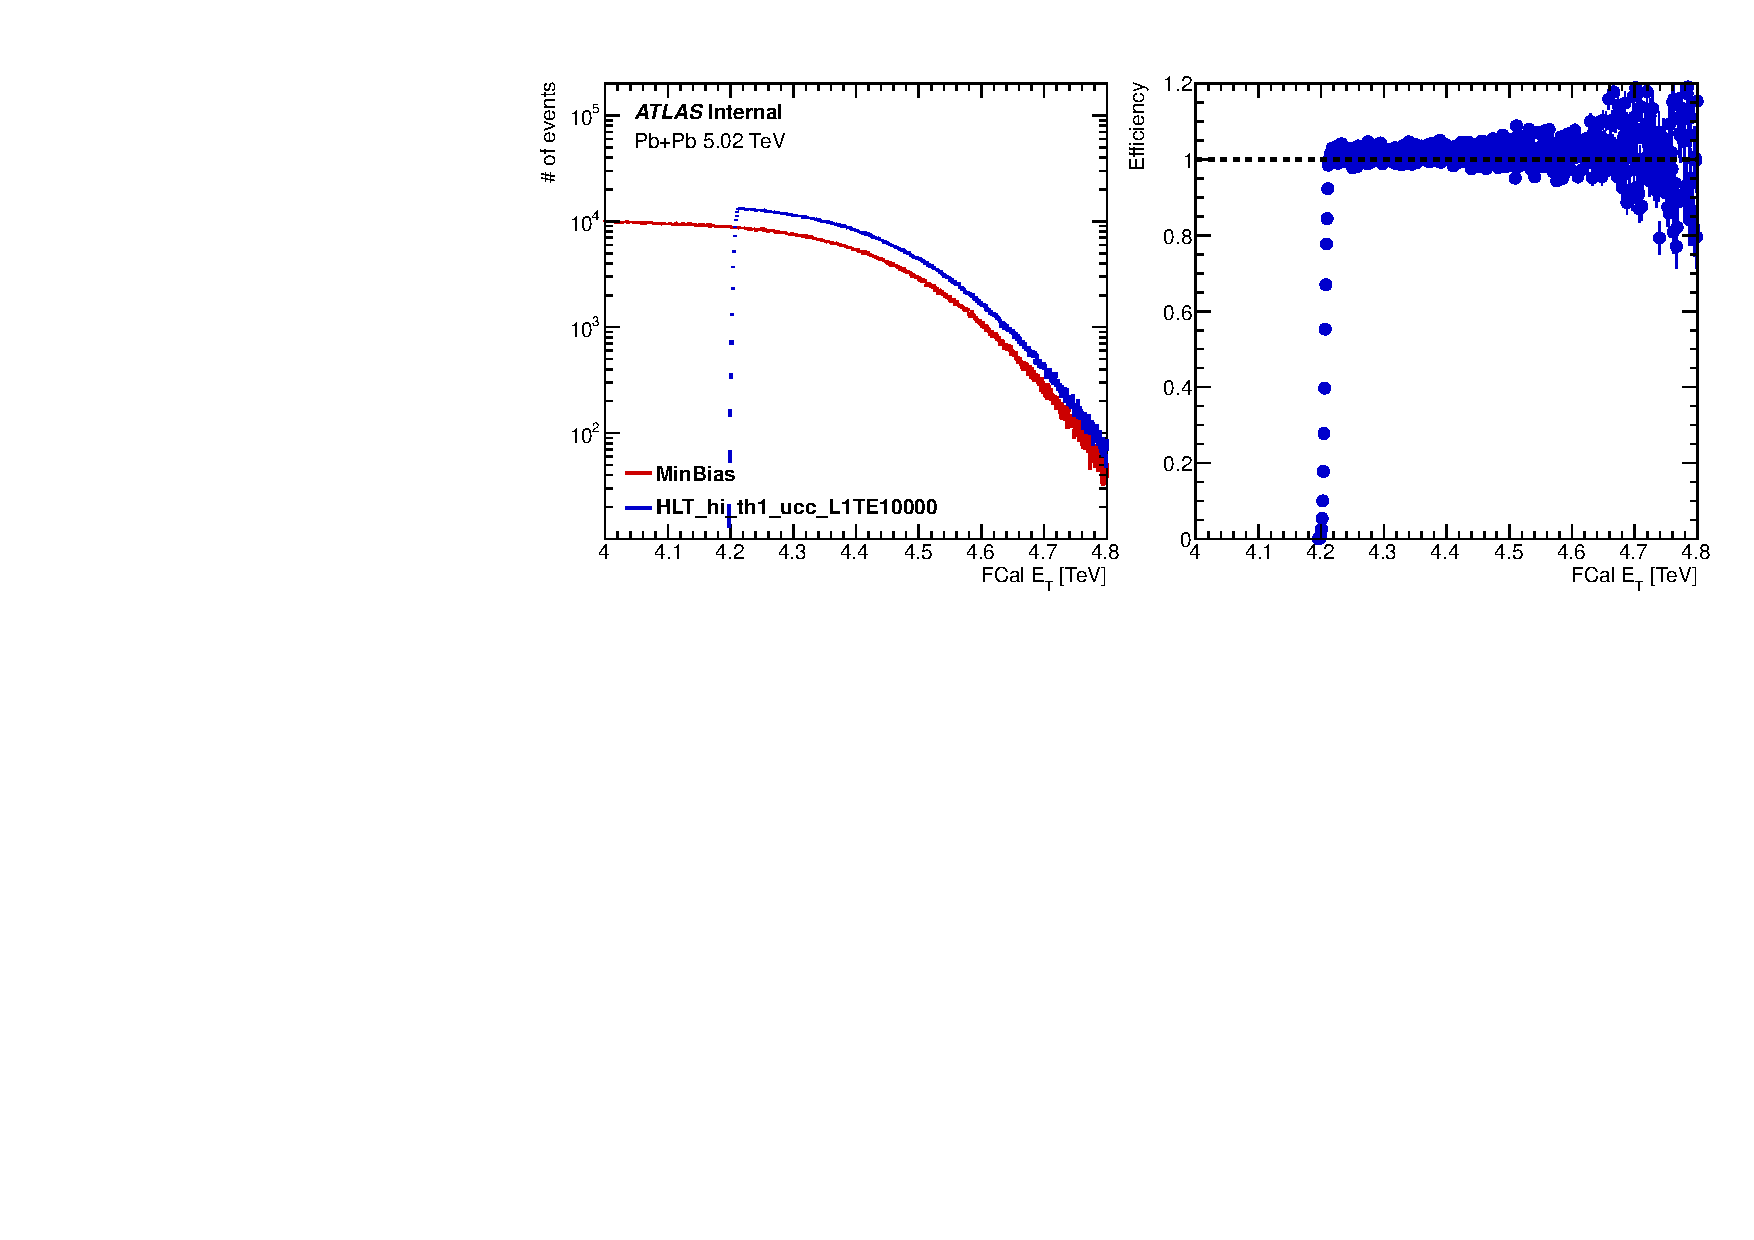
\includegraphics[width=.6\linewidth]{figs/chapter_appendix/trigger_eg1.pdf}
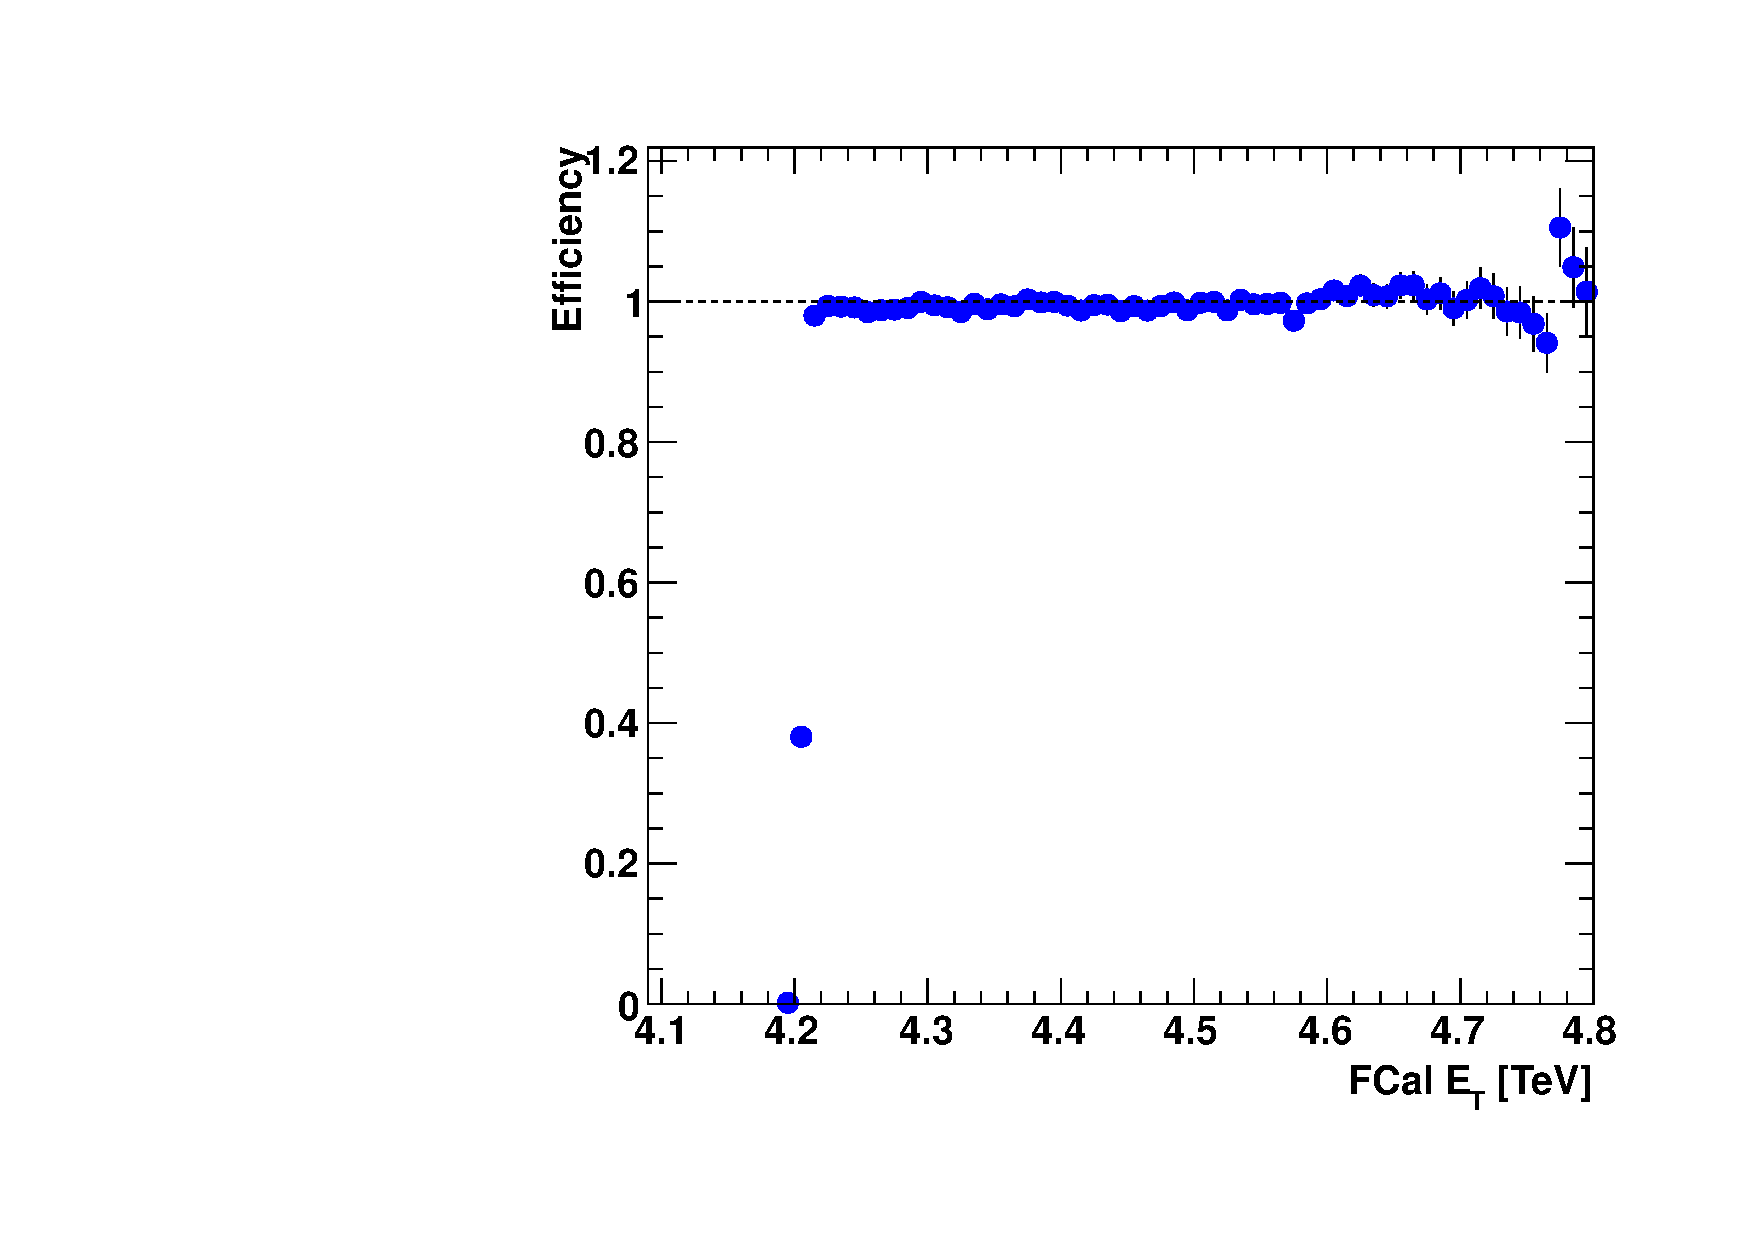
\includegraphics[width=.3\linewidth]{figs/chapter_appendix/trigger_eg2.pdf}
\caption{FCal $\Et$ distributions from MinBias and one UCC trigger (left), trigger "efficiency" as a function of FCal $E_{T}$ (middle) and a zoomed-in version (right) to better see the plateau.}
\label{fig:appendix_trigger_eg}
\end{figure}

In order to evaluate the potential selection bias, we performed the following two checks:
\begin{itemize}
\item Default: include UCC events with efficiency higher than $80\%$;
\item Check: include all UCC events;
\end{itemize}

Fig.~\ref{fig:appendix_trigger} shows the comparison of $c_n\{4\}$ calculated with (default) and without (check) the trigger efficiency selection, as a function of FCal $\Et$ in central collision (Note UCC triggers have no impact on events with centrality $>1\%$). For all the four harmonics, the relative uncertainties are much smaller compared with statistical uncertainties. This is as expected because the turn-on curve of the trigger efficiency is very sharp: not many events are rejected because of the $80\%$ trigger efficiency selection.
\begin{figure}[H]
\centering
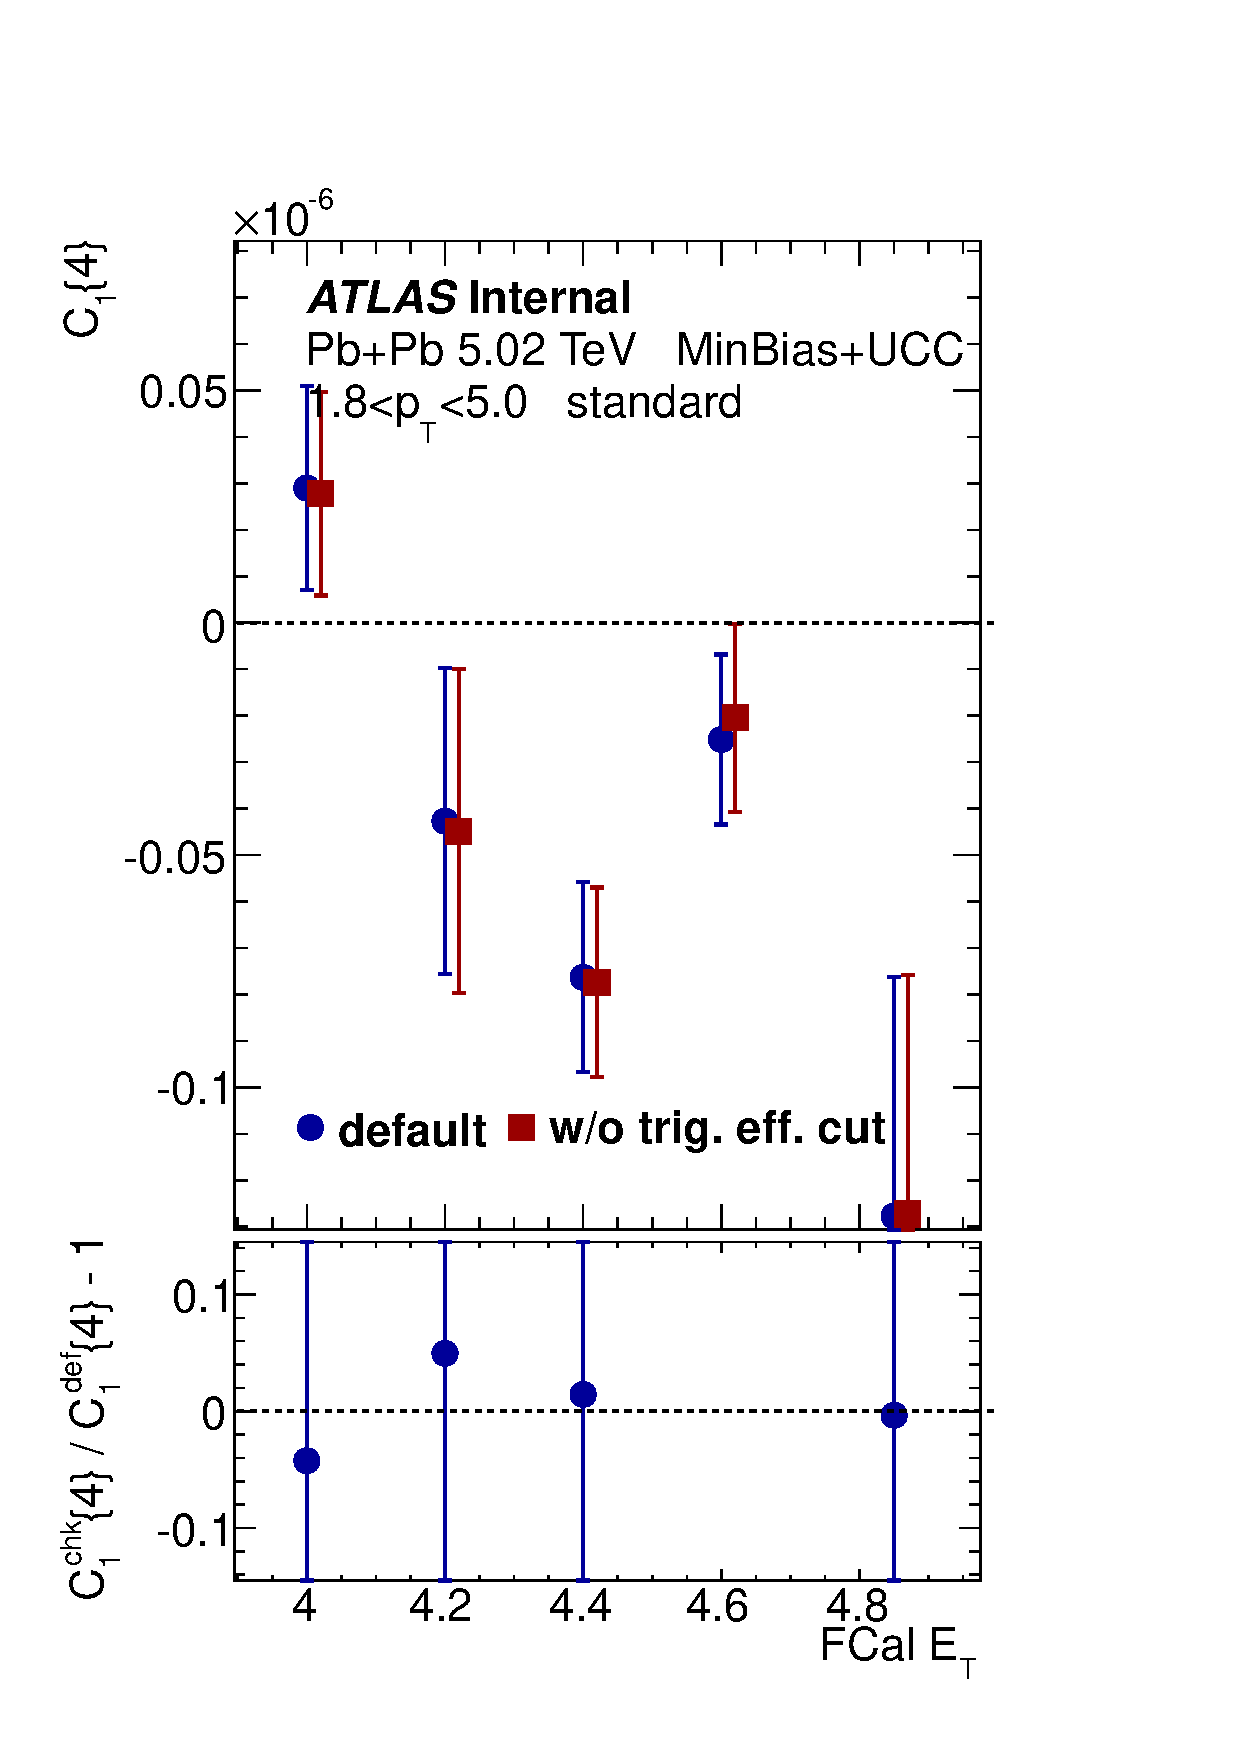
\includegraphics[width=.24\linewidth]{figs/chapter_appendix/trigger_Har1.pdf}
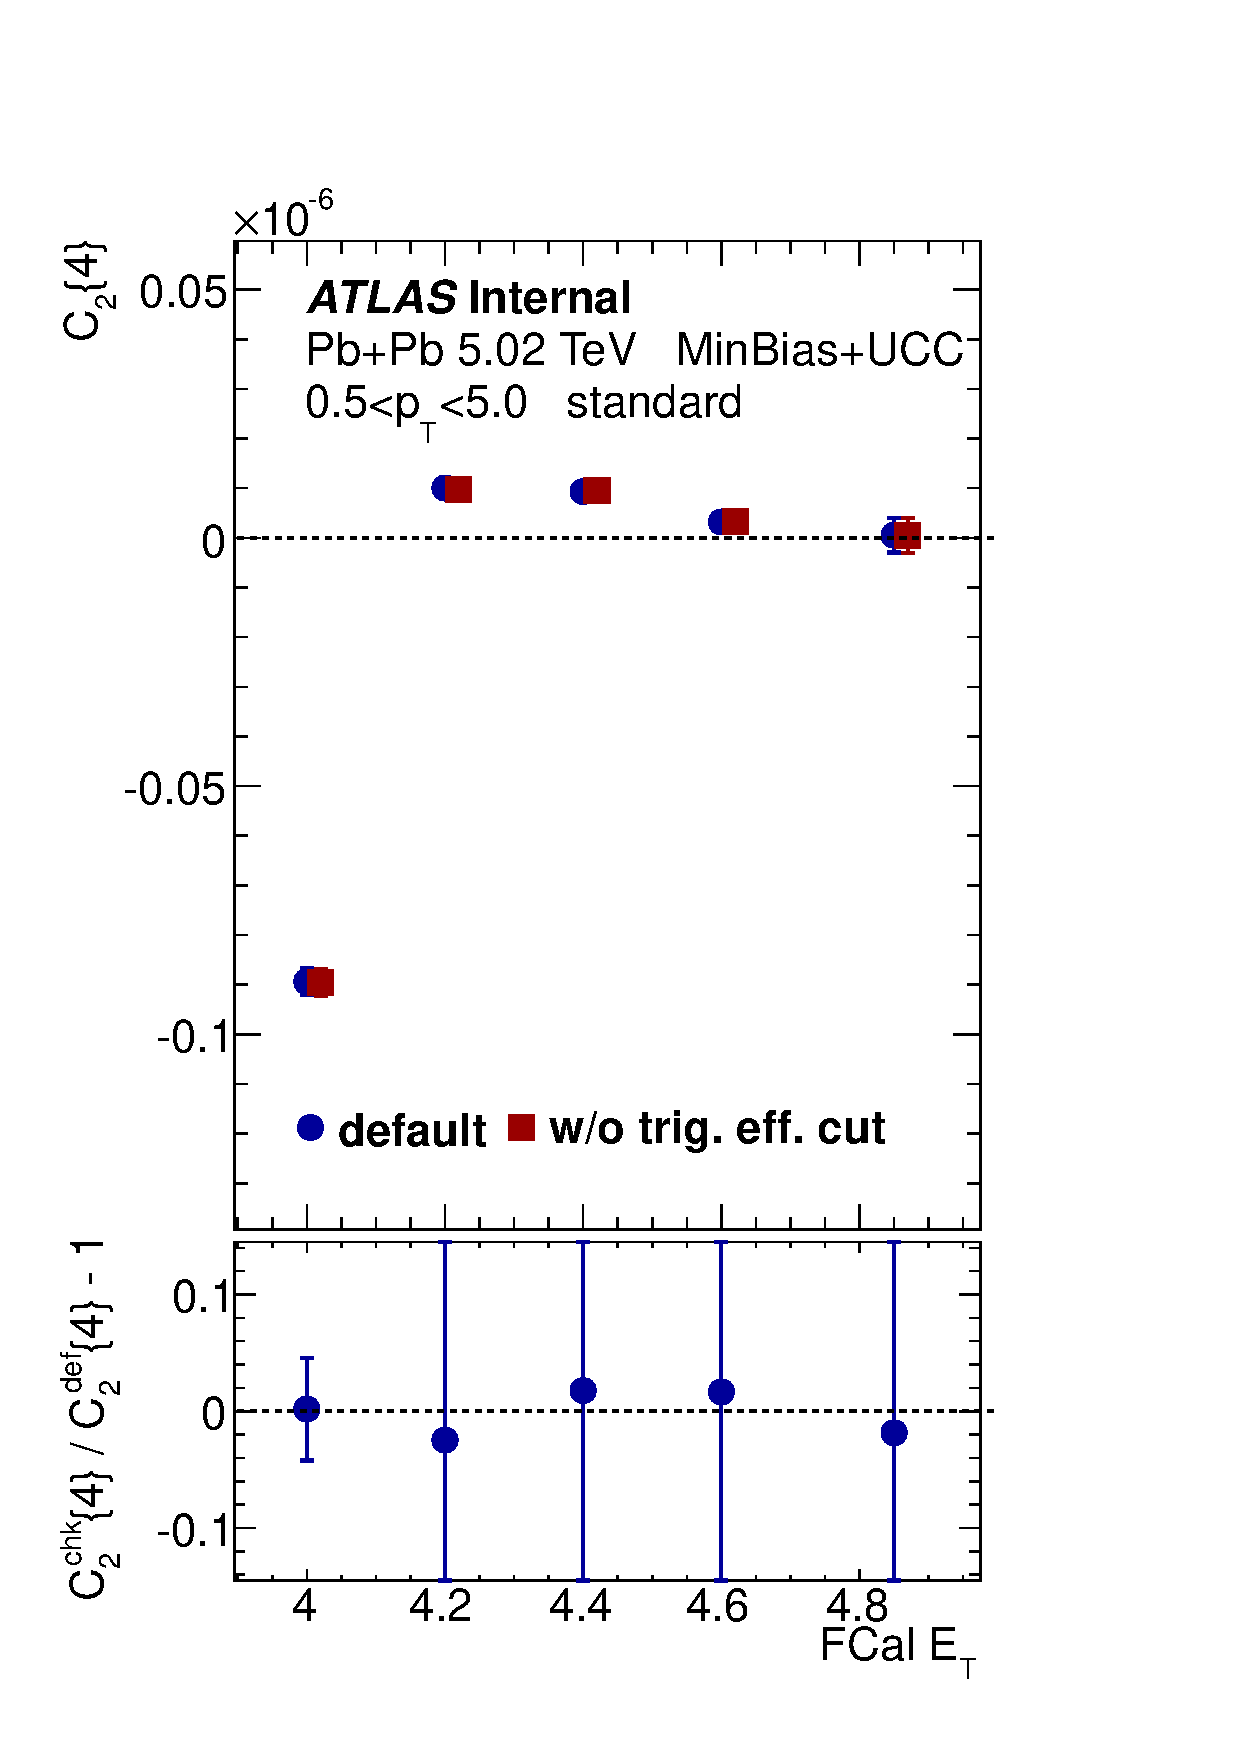
\includegraphics[width=.24\linewidth]{figs/chapter_appendix/trigger_Har2.pdf}
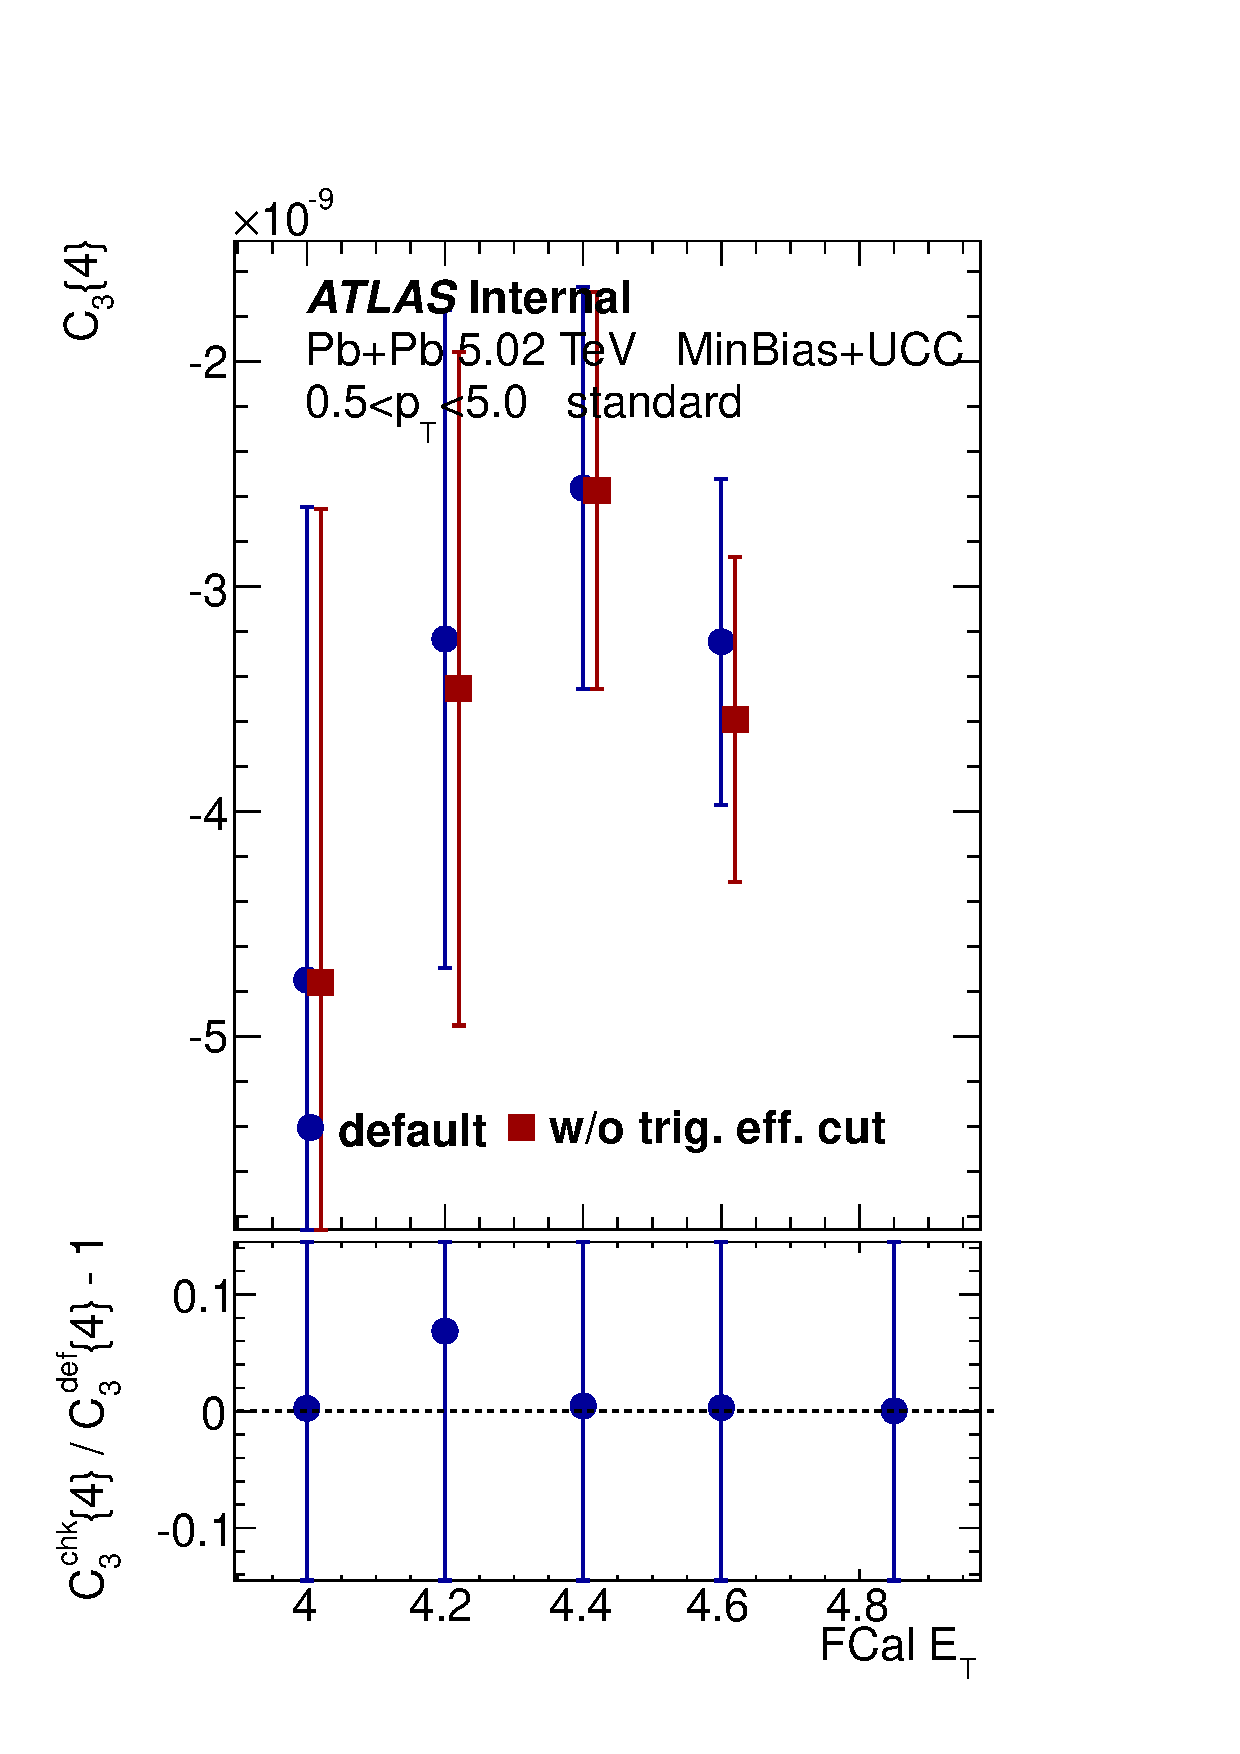
\includegraphics[width=.24\linewidth]{figs/chapter_appendix/trigger_Har3.pdf}
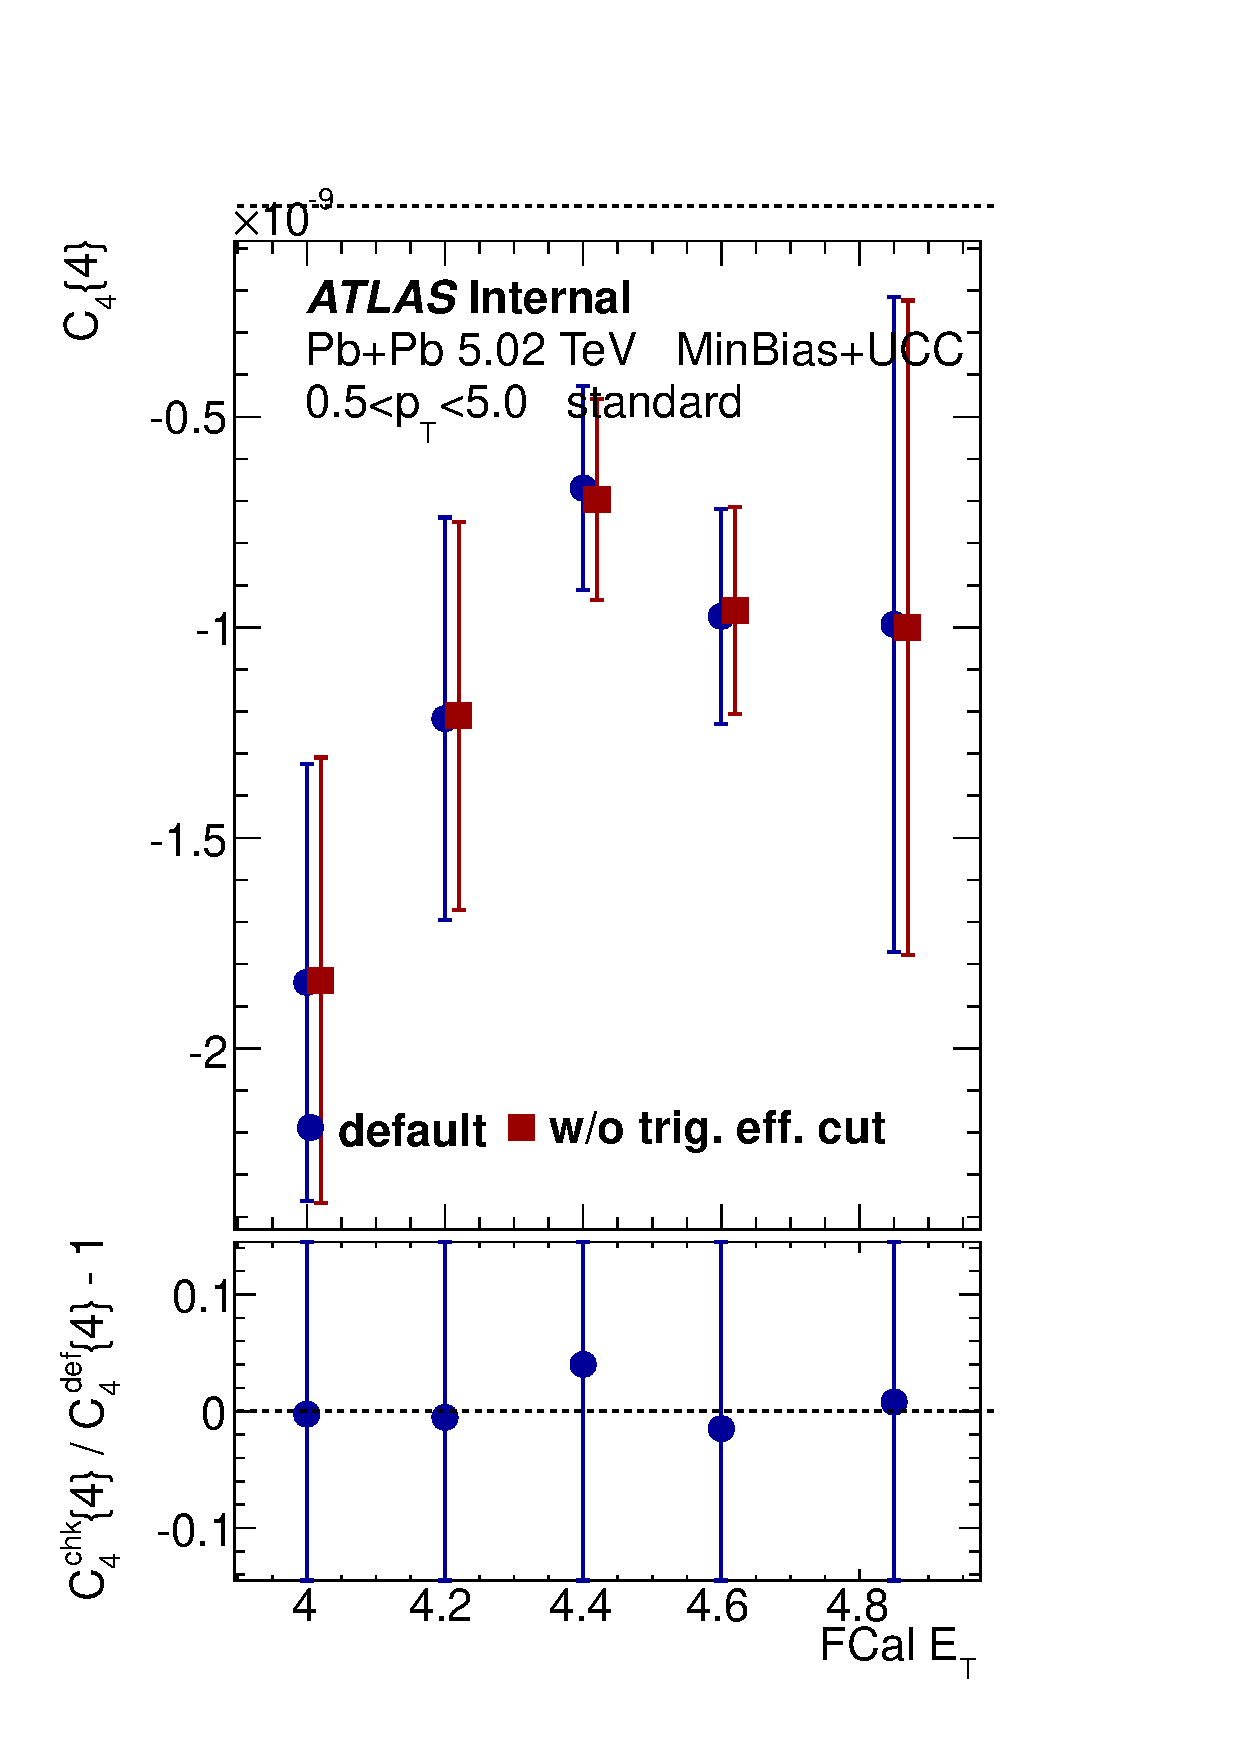
\includegraphics[width=.24\linewidth]{figs/chapter_appendix/trigger_Har4.pdf}
\caption{Systematics of $c_n\{4\}$ from UCC trigger efficiency: with v.s. without trigger efficiency cut. Bottom panels are the relative uncertainties between the default and check.}
\label{fig:appendix_trigger}
\end{figure}



\subsubsection{Pileup rejection}
\label{sec:pileup_rejection}

During the 2015 Pb+Pb data taking, the mean value of $\mu$ is around 0.001, which means the fraction of pileup events is very low compared with $pp$ or $p+$Pb samples. Furthermore, in this analysis all the tracks used to calculate cumulants are from the primary vertex. In principle, in pile-up events, tracks from pile-up vertex should not contribute to the measurement. However, in the track and vertex reconstruction, when a pile-up vertex is too close to the primary vertex, two vertices might be merged. Since the particles from two different vertices are totally uncorrelated, including these events with merged vertex will reduce the signal of flow signal.

In order to check the impact from pileup events, a variation of pileup cleaning is performed:
\begin{itemize}
\item Default: official HI pileup rejection tool, based on FCal $\Et$ and ZDC;
\item Check: alternative pileup rejection method, based on FCal $\Et$ and tracks $\Nch$;
\end{itemize}

Fig.~\ref{fig:appendix_pileup_eg} illustrates the differences between the two pileup cleaning methods: official (left) and alternative (right). The left panel shows the correlation between FCal sum $\Et$ and calibrated number of neutrons in the ZDC. The main band (light blue circle) is dominated by the events with a single primary vertex and the "grass" above the main band (light red circle) are mainly from pileup events. This is because both the sum $\Et$ and number of neutrons in a pileup event are larger than the corresponding single event. In order to clean up the pileup events, a significance cut (indicated by the red curve) was applied to reject the top $0.1\%$ events at each FCal sum $\Et$ slice. From this correlation map, it is obvious that the pileup events and single events are disentangled at very high FCal sum $\Et$, meaning that almost all the pileup events are rejected with the official pileup tool. As a comparison, the right panel shows the correlation between FCal sum $\Et$ and the number of tracking efficiency corrected reconstructed tracks $\Nch$. Similar as the left panel, the "grass" under the main band are from the pileup events. However, since FCal sum $\Et$ and $\Nch$ are correlated, the overlap region between the pileup events and single events is much larger than the previous case, where the $N_\text{neutron}$ and FCal sum $\Et$ are anti-correlated. This means the performance of this alternative pileup rejection method is much worse than the official, which provides sufficient variations as a cross-check.
\begin{figure}[H]
\centering
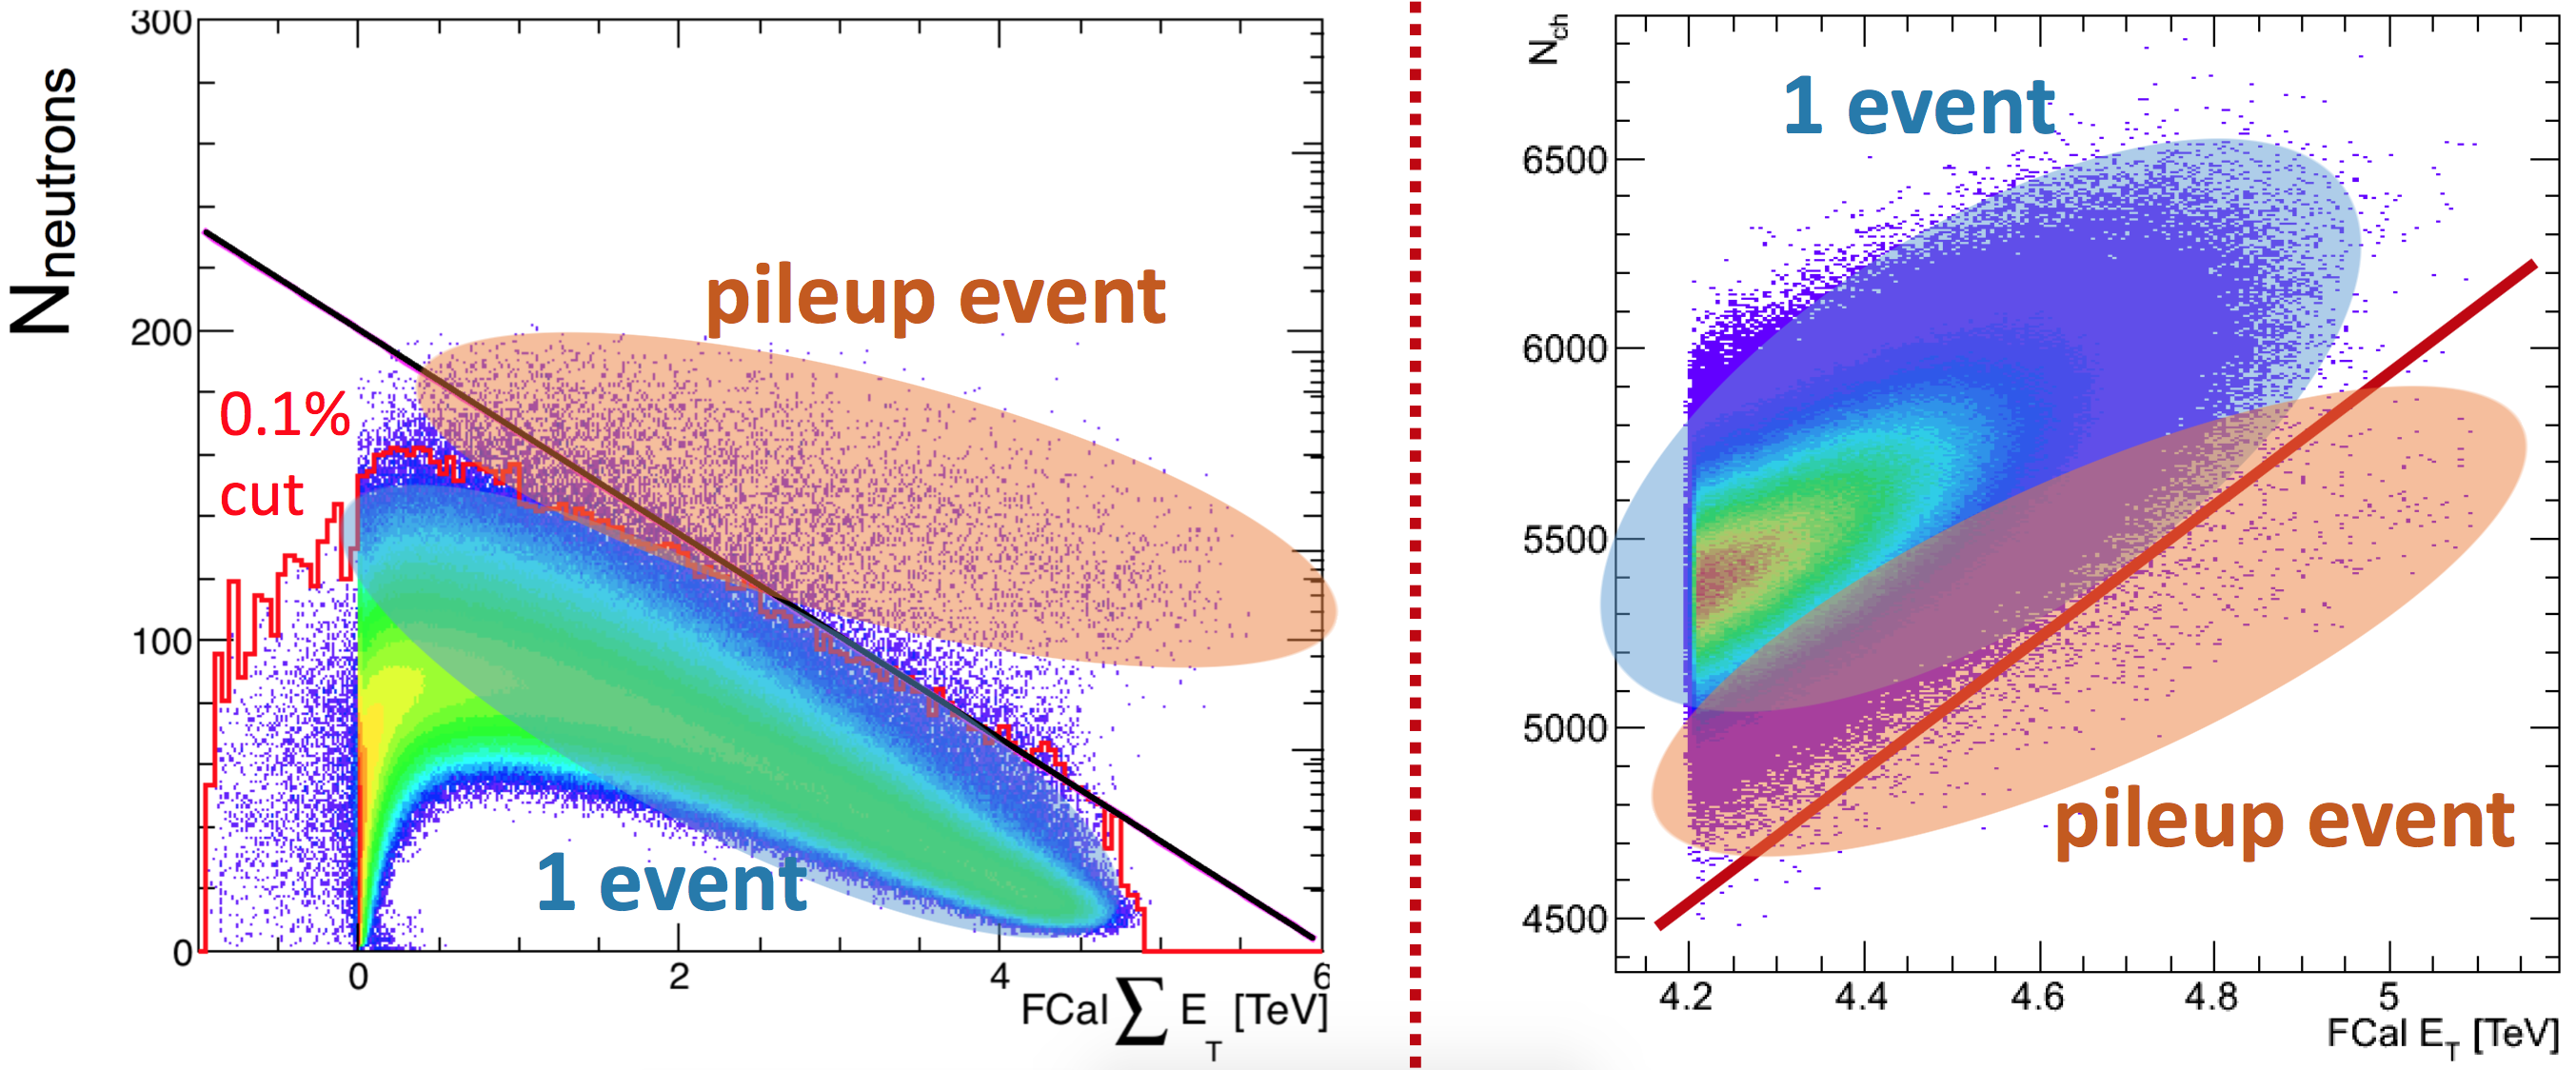
\includegraphics[width=.9\linewidth]{figs/chapter_appendix/pileup_eg.png}
\caption{An illustration of two pileup rejection methods: official HI pileup tool (left) and private pileup rejection (right).}
\label{fig:appendix_pileup_eg}
\end{figure}

The fraction of pileup events in peripheral is minimal and it increases fast with FCal $\Et$, so only comparisons in UCC events are shown. But note that this systematic check is also performed for the whole centrality range. It is worth mentioning that this check overestimates the pileup impact since the fraction of residual pileup events are large using the alternative rejection. Another way to estimate the impact from pileup would be by adjusting the significance cut of $N_\text{neutrons}$, and check the trend of $c_n\{4\}$ as a function of various ZDC energy cut. To be conservative, we are quoting the difference between the two methods as the upper bond of the systematics for pileup effects.

The comparison of $c_n\{4\}$ calculated with and without pileup rejection is shown in Fig.~\ref{fig:appendix_pileup}, as a function of FCal $\Et$ in ultra-central collisions. For all the harmonics, the relative differences are within $10\%$ and within statistical uncertainties. It is quoted as part of the systematics.

\begin{figure}[H]
\centering
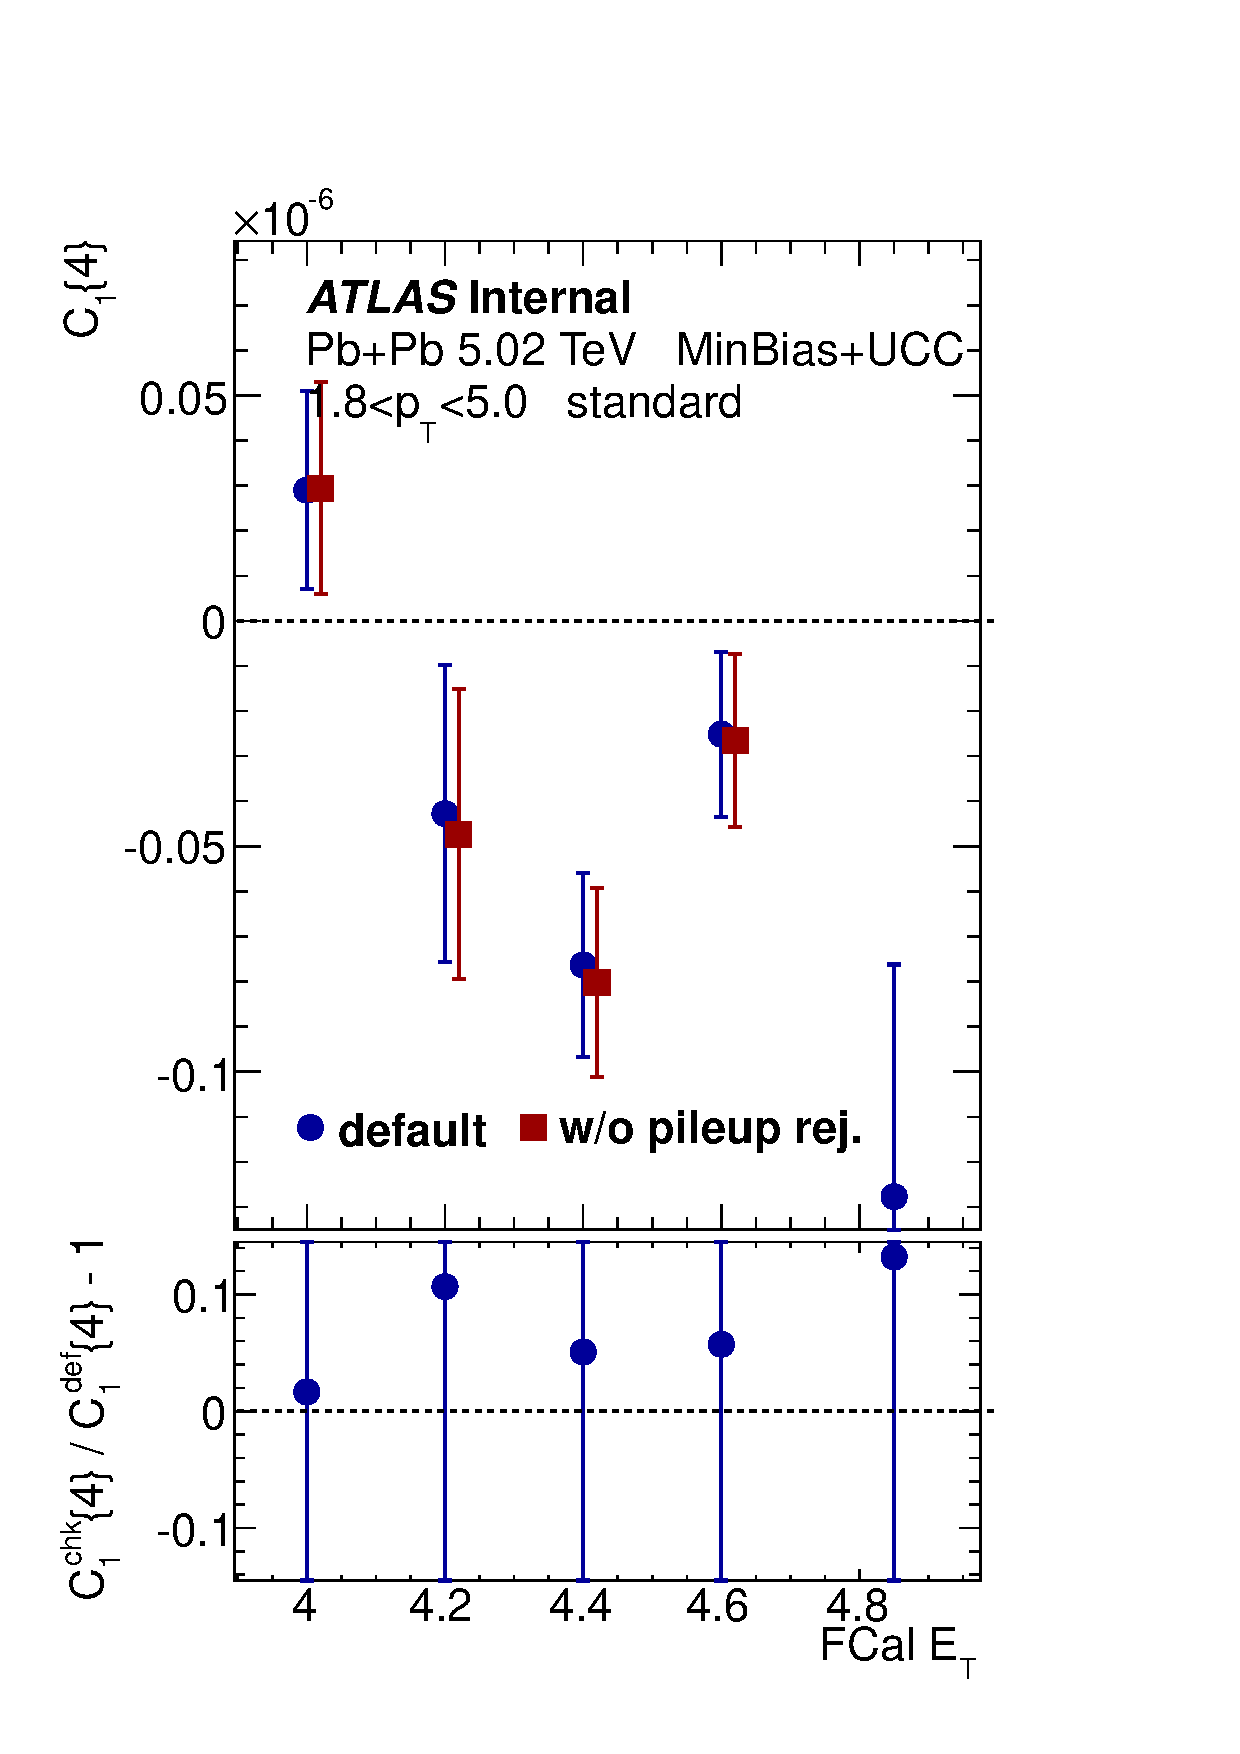
\includegraphics[width=.24\linewidth]{figs/chapter_appendix/pileup_Har1.pdf}
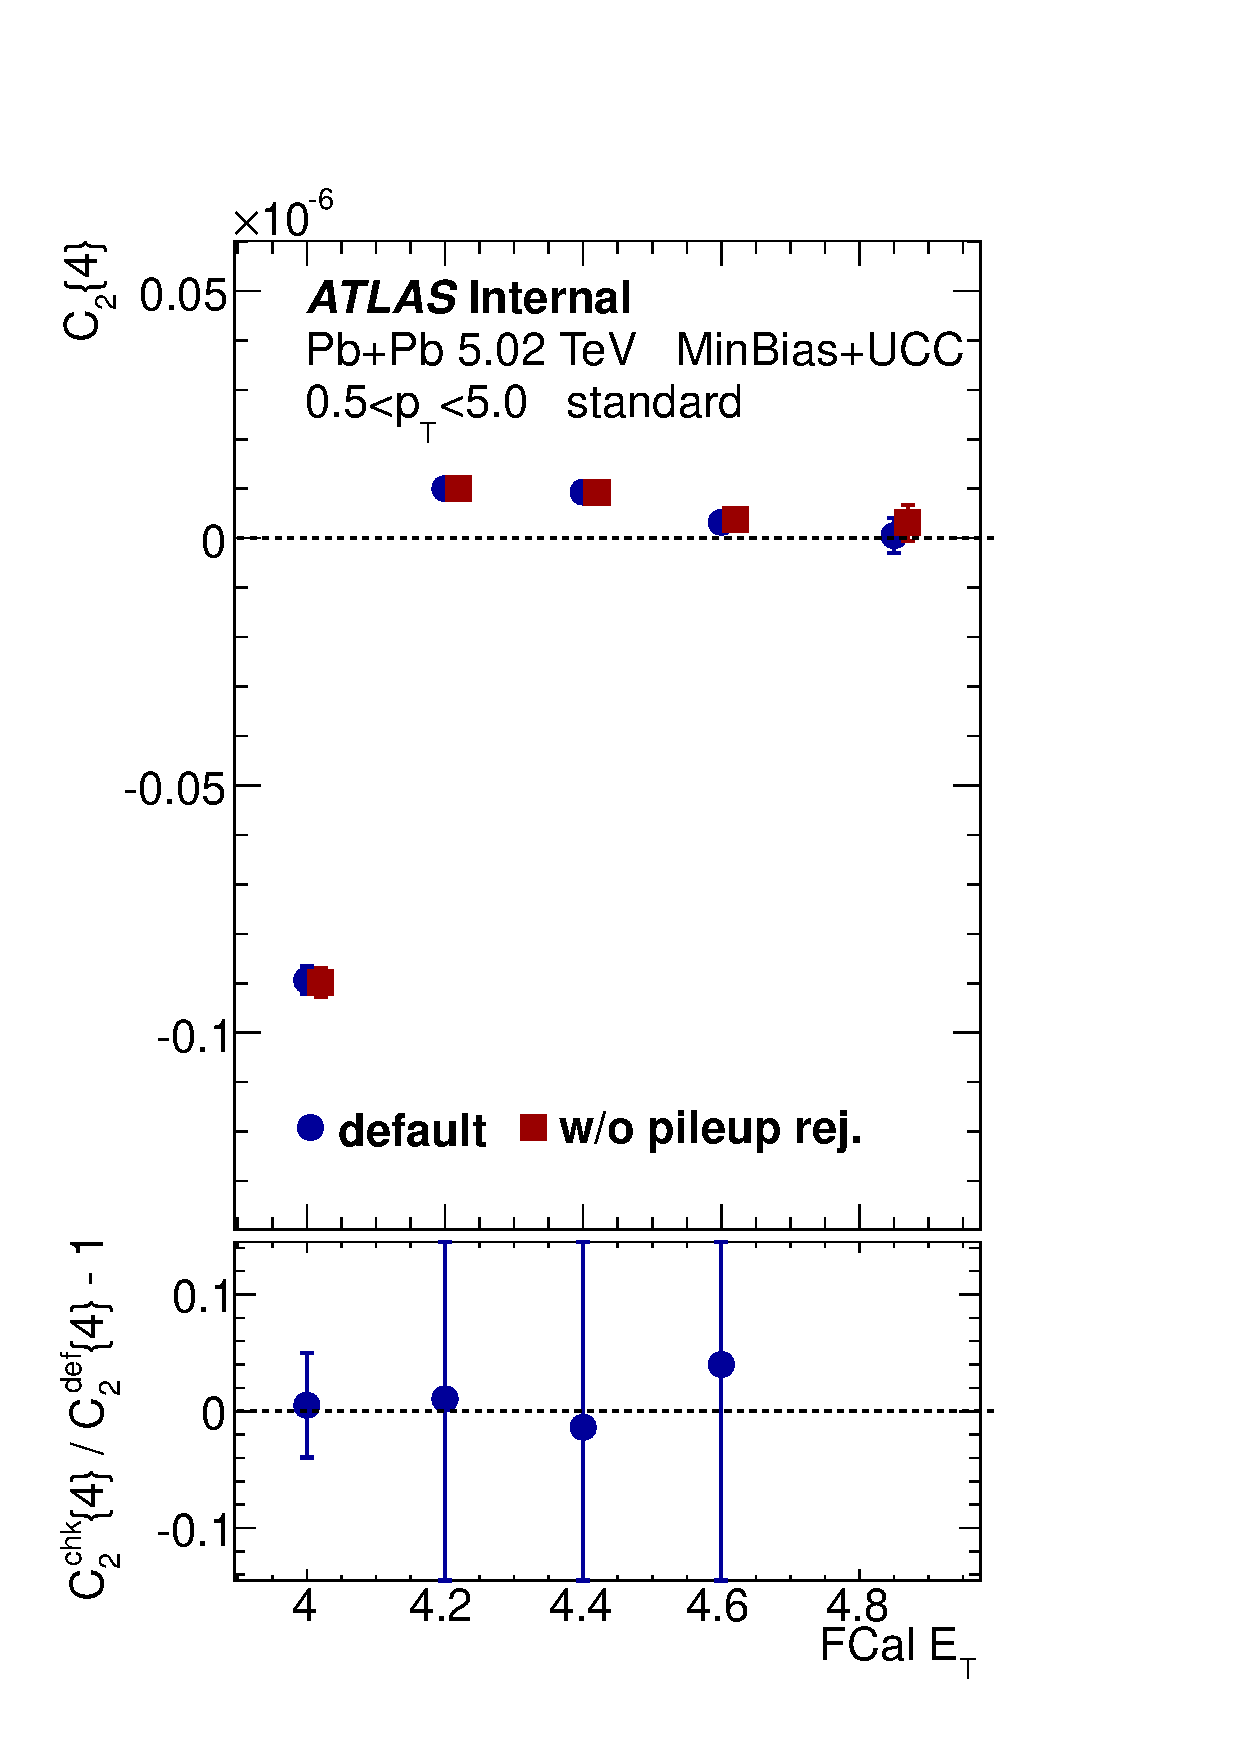
\includegraphics[width=.24\linewidth]{figs/chapter_appendix/pileup_Har2.pdf}
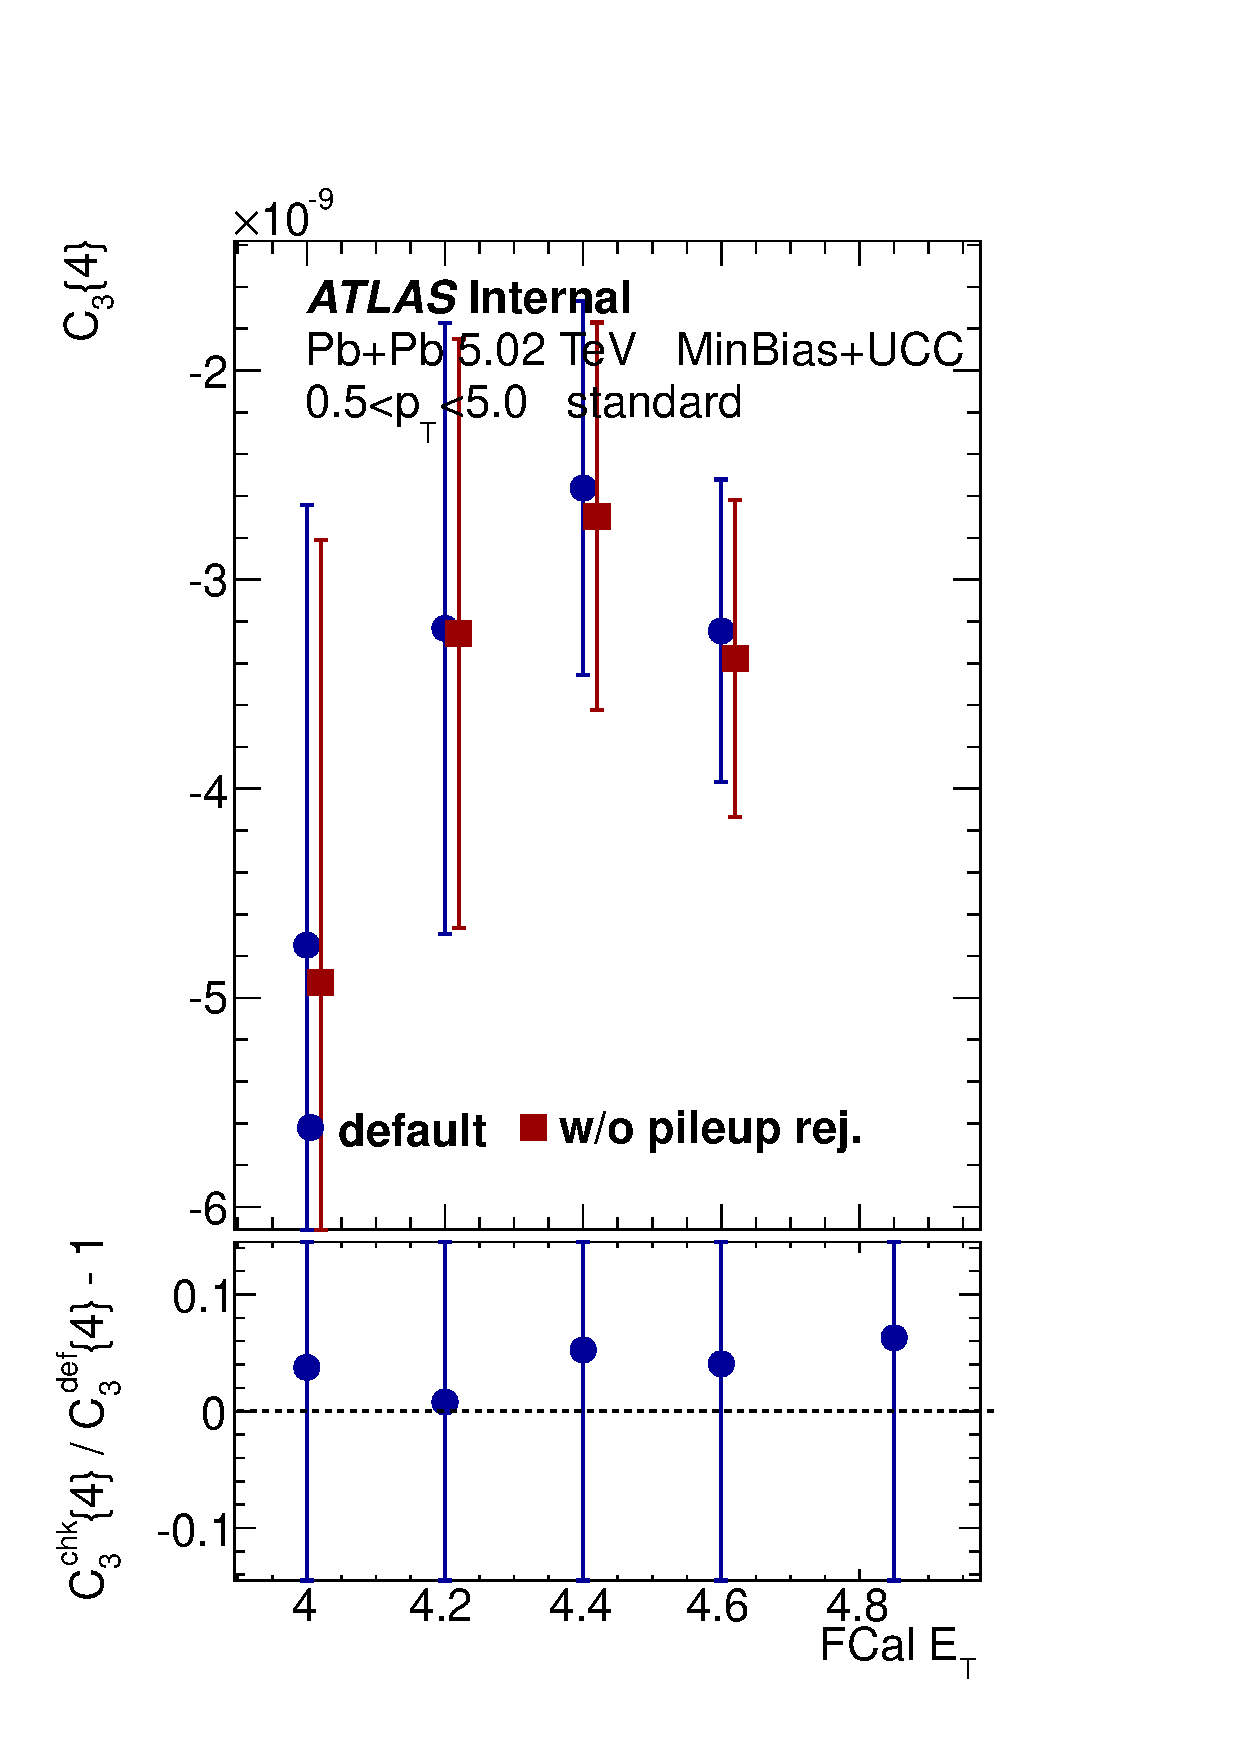
\includegraphics[width=.24\linewidth]{figs/chapter_appendix/pileup_Har3.pdf}
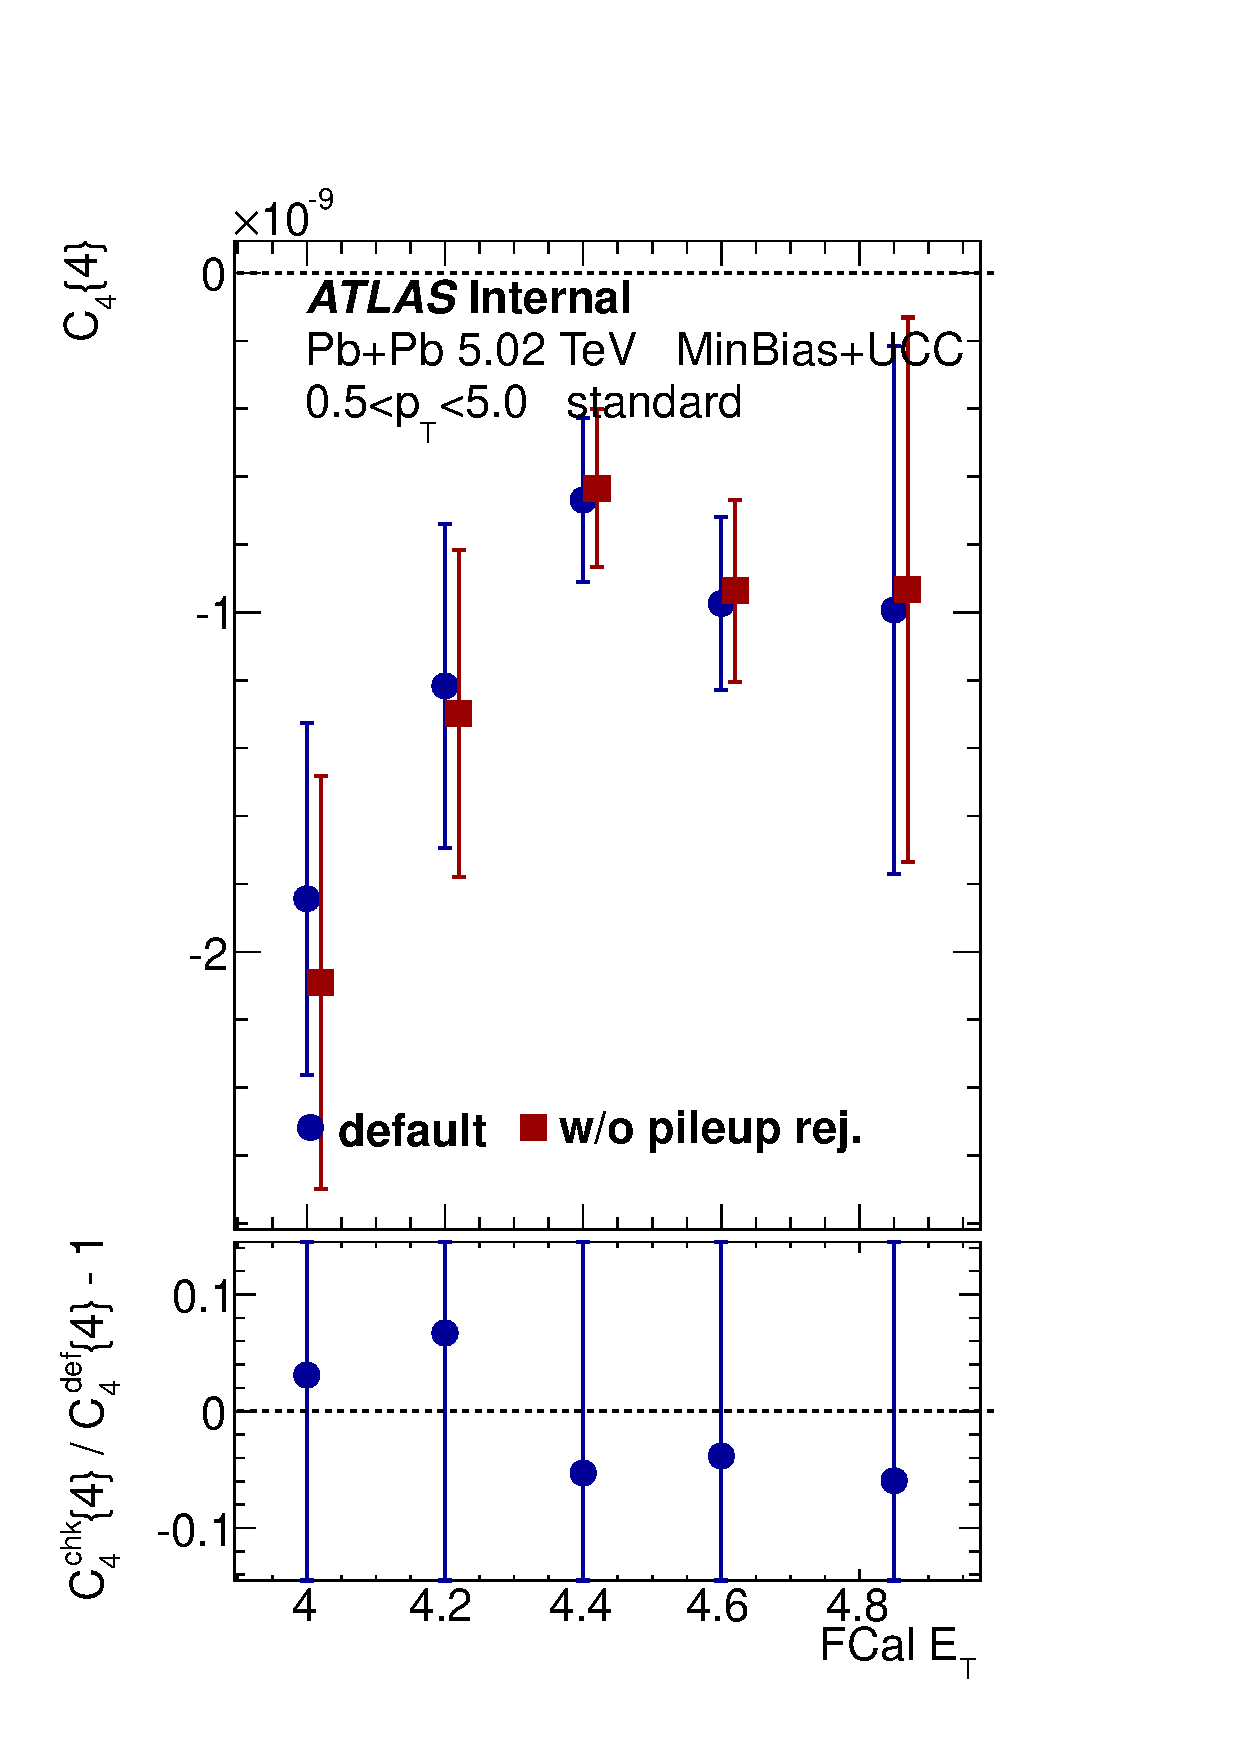
\includegraphics[width=.24\linewidth]{figs/chapter_appendix/pileup_Har4.pdf}
\caption{Systematics of $c_n\{4\}$ from pileup effects: with different pileup rejection criteria. Bottom panels are the relative uncertainties between the default and check.}
\label{fig:appendix_pileup}
\end{figure}



\subsubsection{Centrality definition}
\label{sec:centrality_definition}

Uncertainty in how well the min-bias triggers sample the Pb+Pb cross-section (i.e. the min-bias trigger efficiency) results in an uncertainty in the definition of the centrality intervals. This causes the nominal $(0-85)\%$ centrality range to have a $\pm 1\%$ uncertainty. The effect of such uncertainties on observables are determined by re-evaluating the observables with the following criteria:
\begin{itemize}
\item Default: $(0-85)\%$ centrality range;
\item Check 1: $(0-84)\%$ centrality range;
\item Check 2: $(0-86)\%$ centrality range;
\end{itemize}

Fig.~\ref{fig:appendix_centrality} compares the $c_n\{4\}$ for the different centrality ranges. This systematic uncertainty depends on the centrality dependence of the observable: if the observable has no centrality dependence, the uncertainty is zero. On the other hand, this uncertainty is large if the observable is strongly dependent of centrality. This explains why this uncertainty for $c_3\{4\}$ is larger than that of $c_2\{4\}$. Different $\pT$ ranges make little difference since the relative centrality dependence of the observables do not change much.
\begin{figure}[H]
\centering
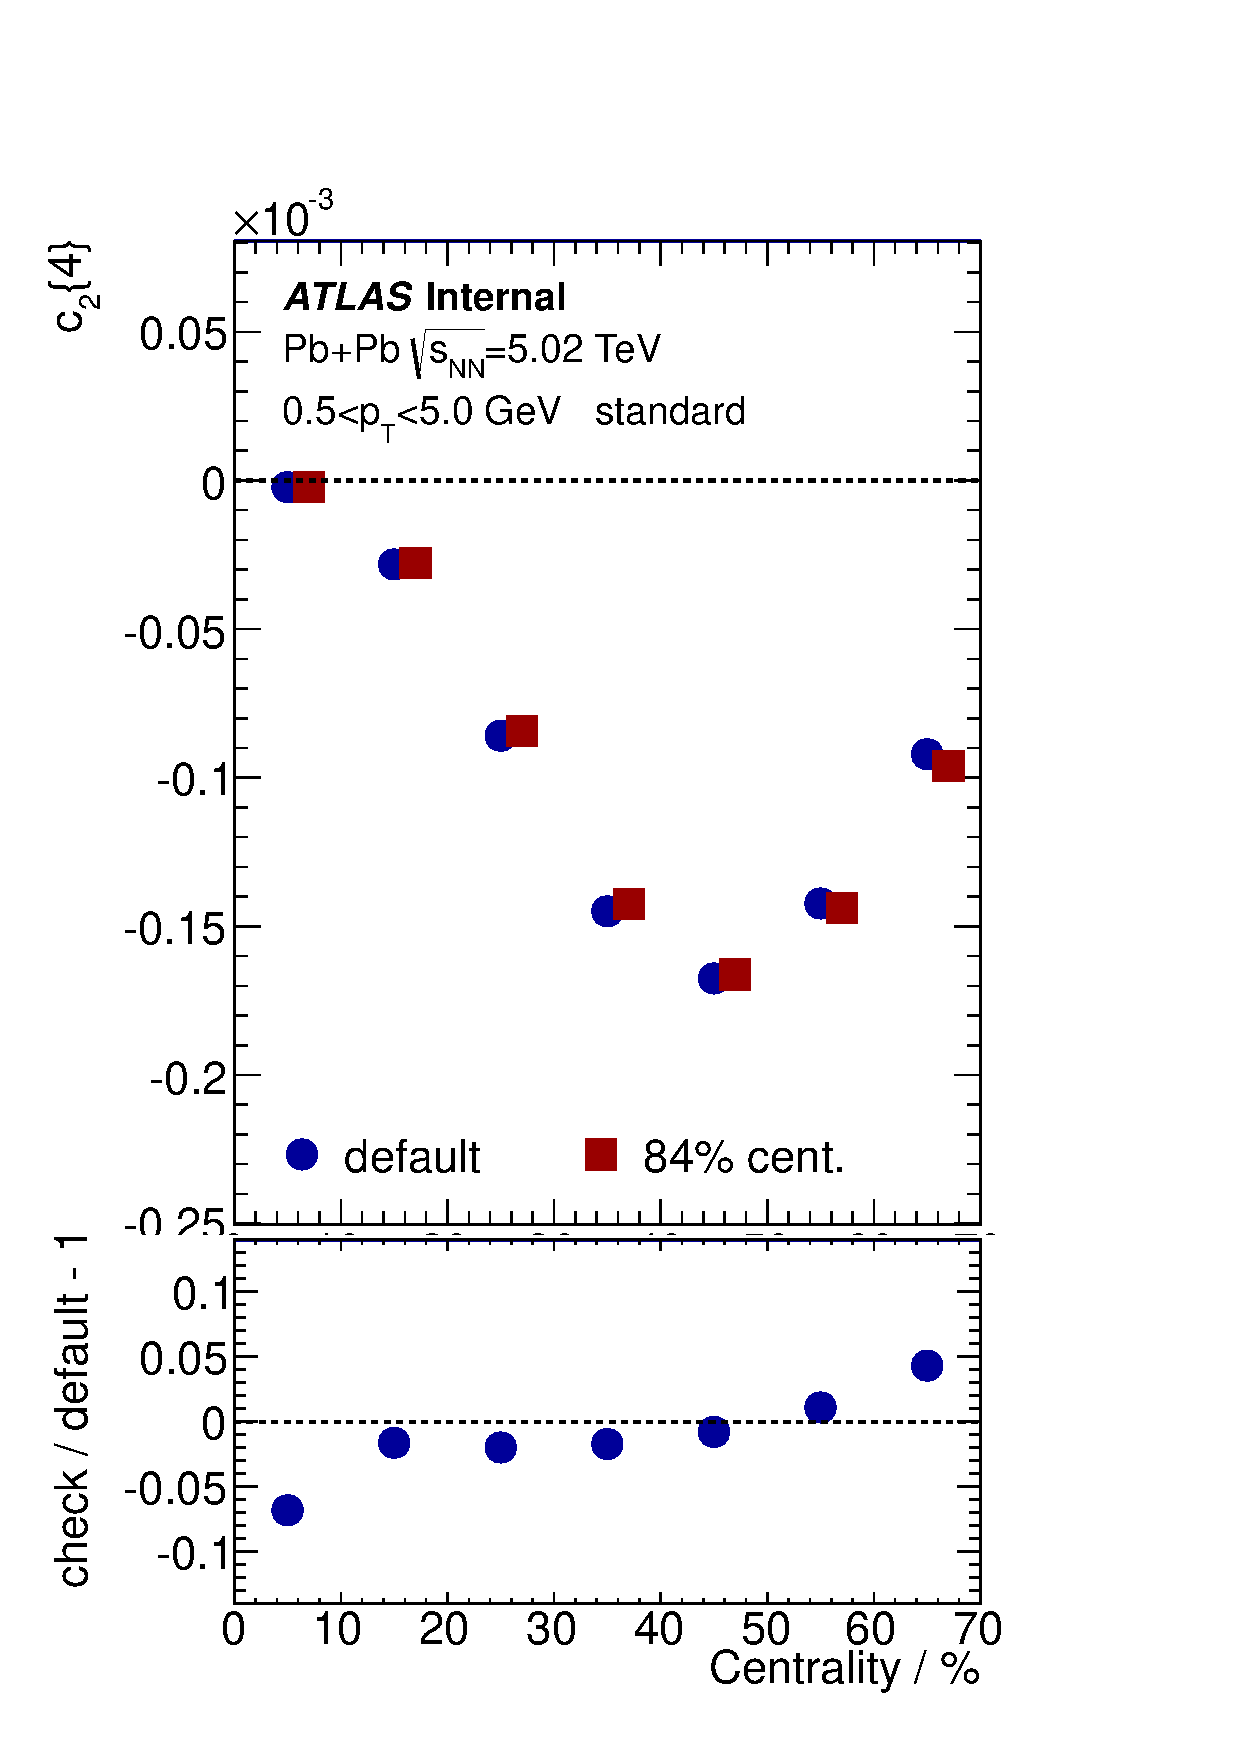
\includegraphics[width=.24\linewidth]{figs/chapter_appendix/centrality_Har2_Pt0.pdf}
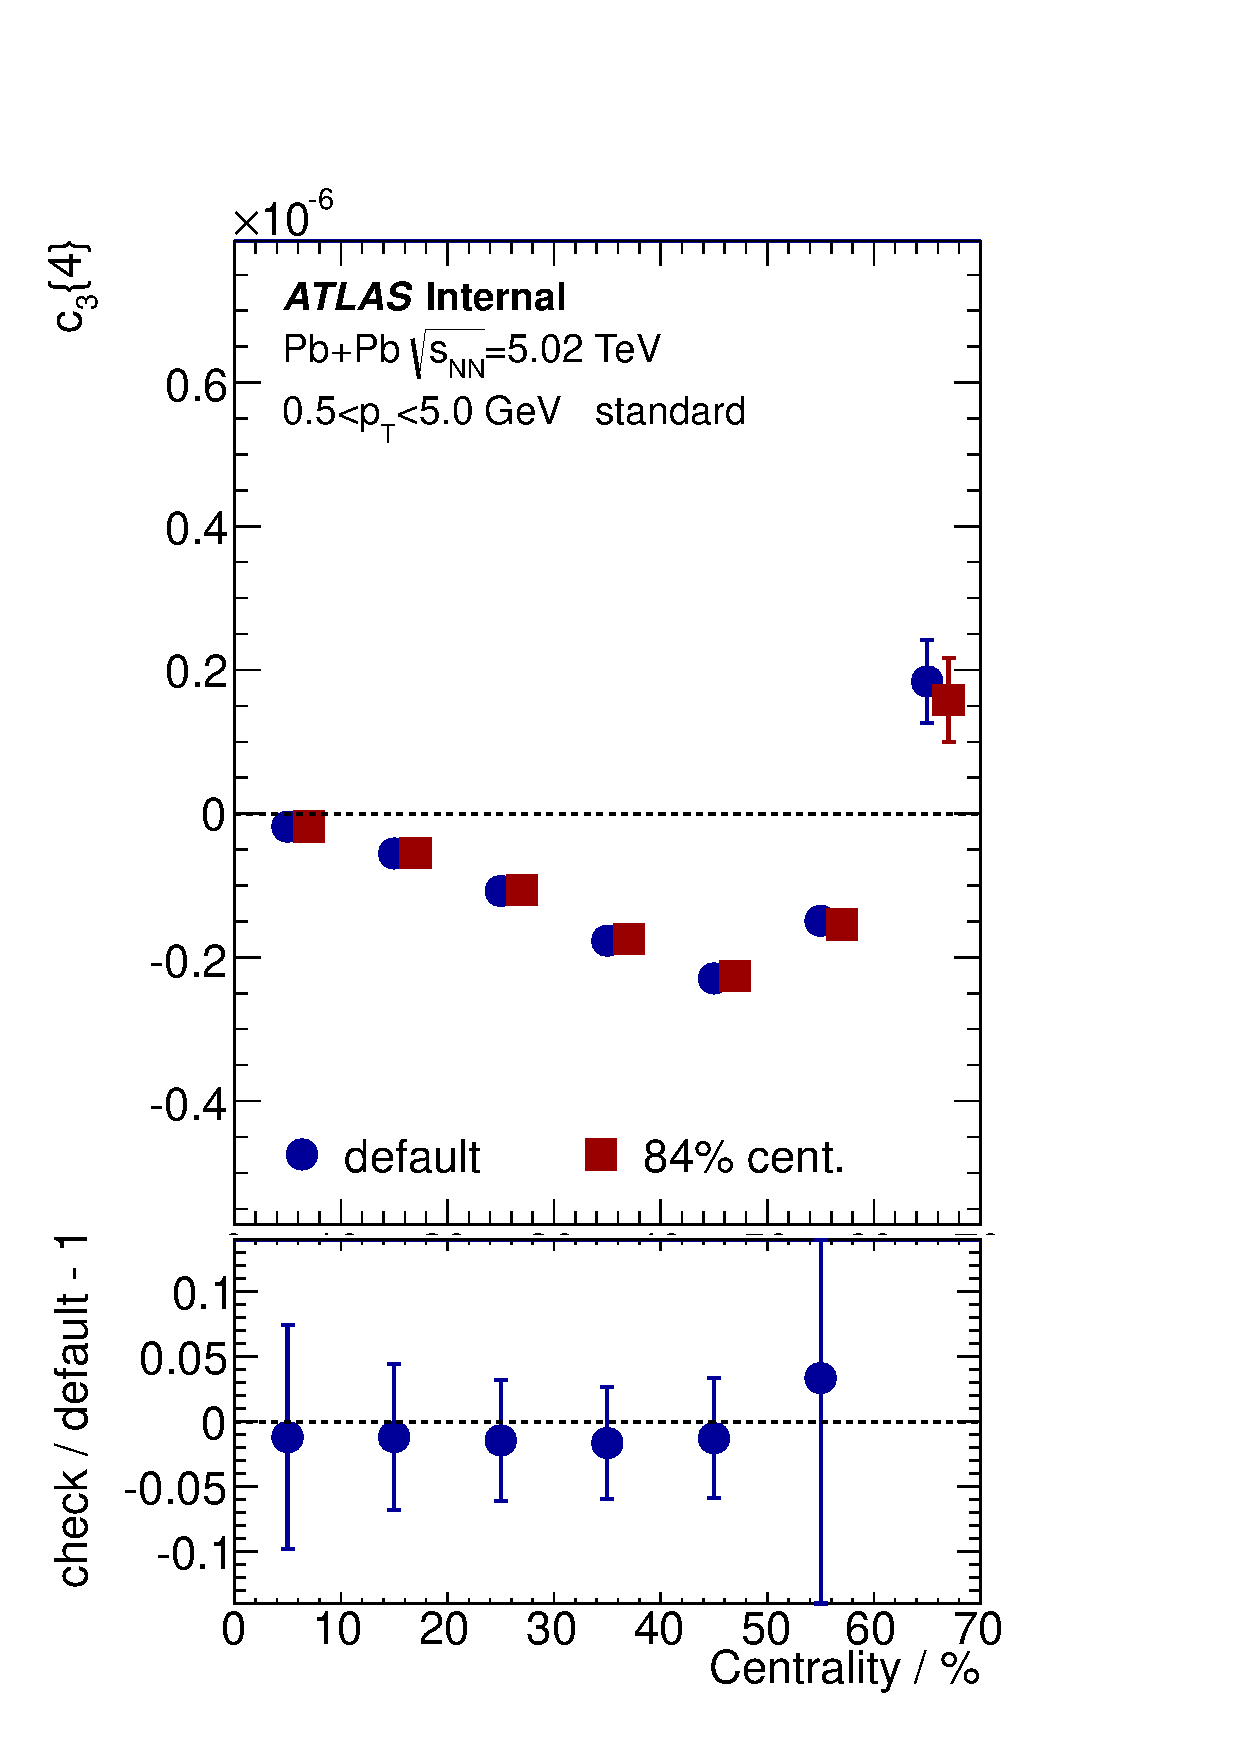
\includegraphics[width=.24\linewidth]{figs/chapter_appendix/centrality_Har3_Pt0.pdf}
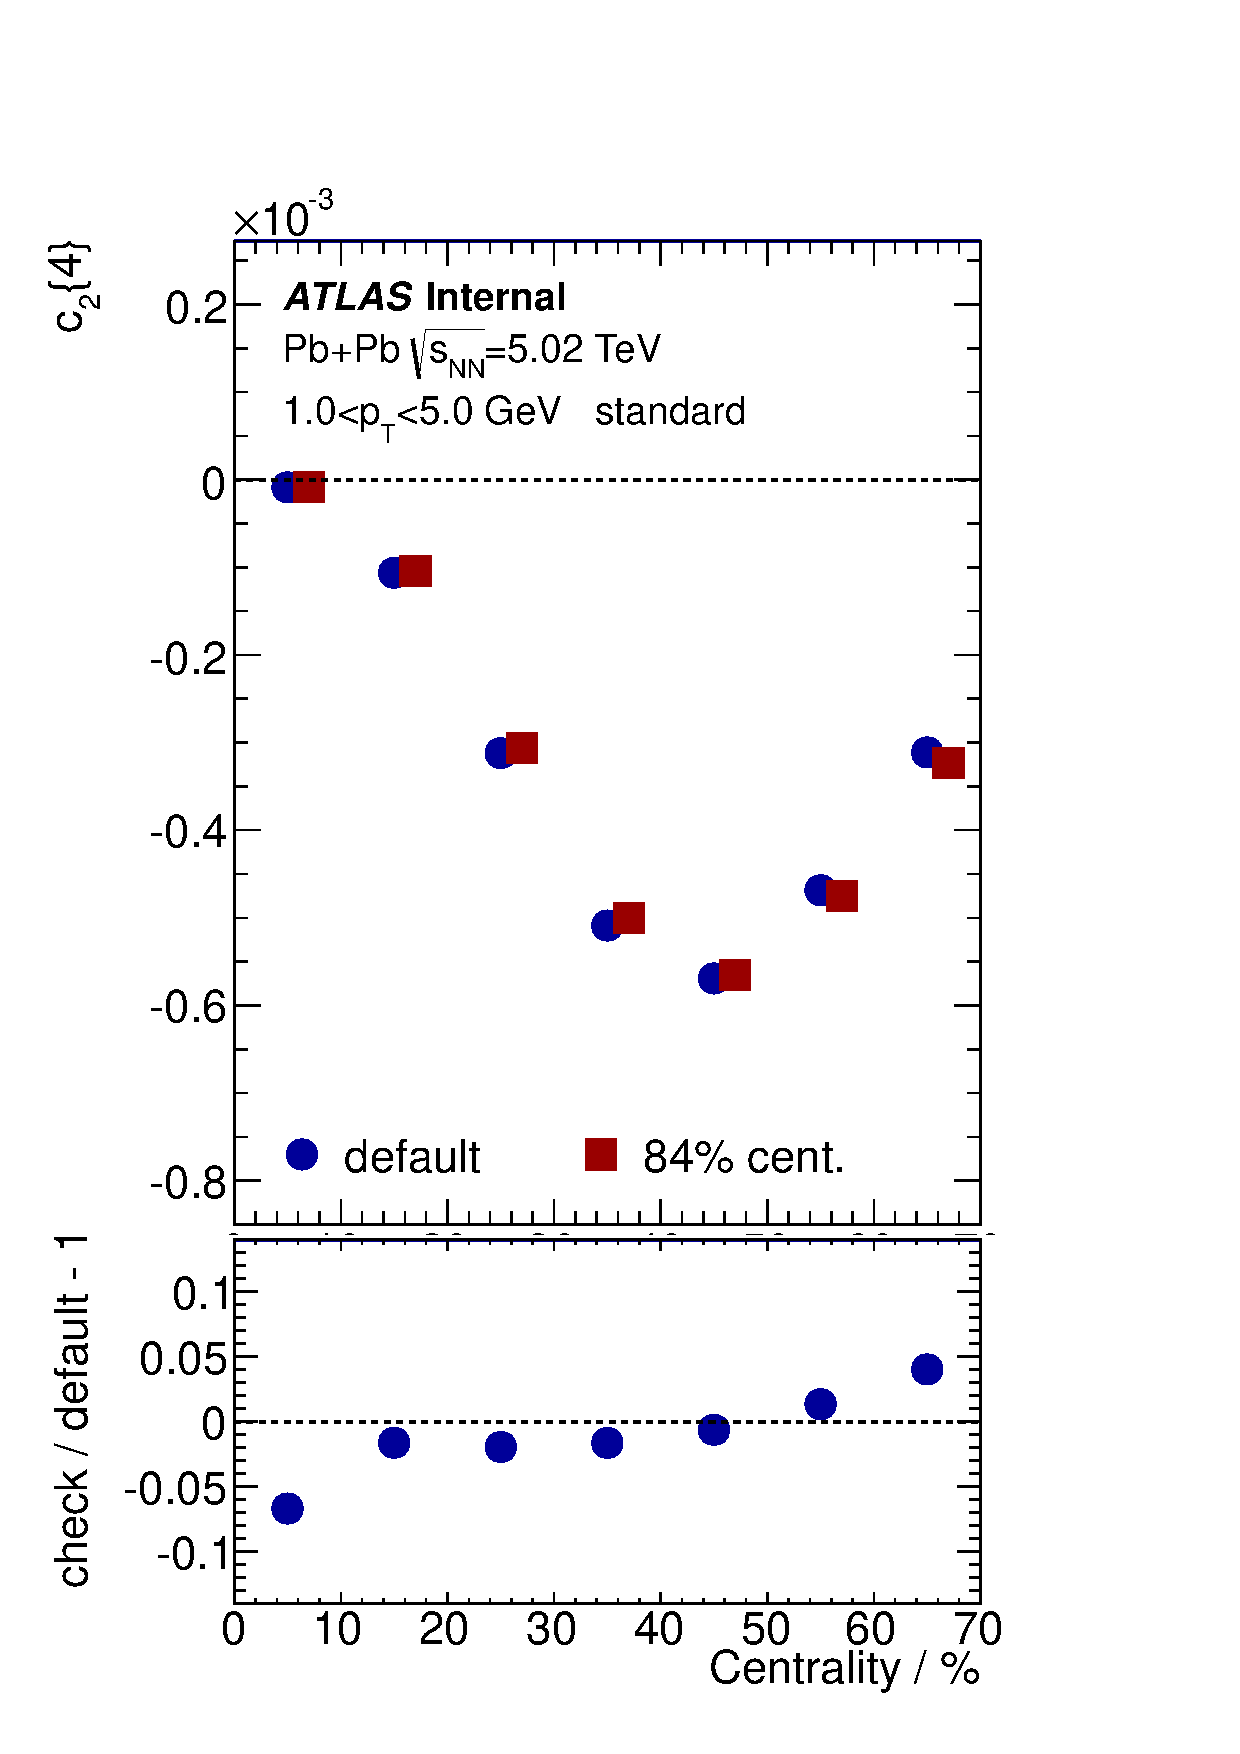
\includegraphics[width=.24\linewidth]{figs/chapter_appendix/centrality_Har2_Pt1.pdf}
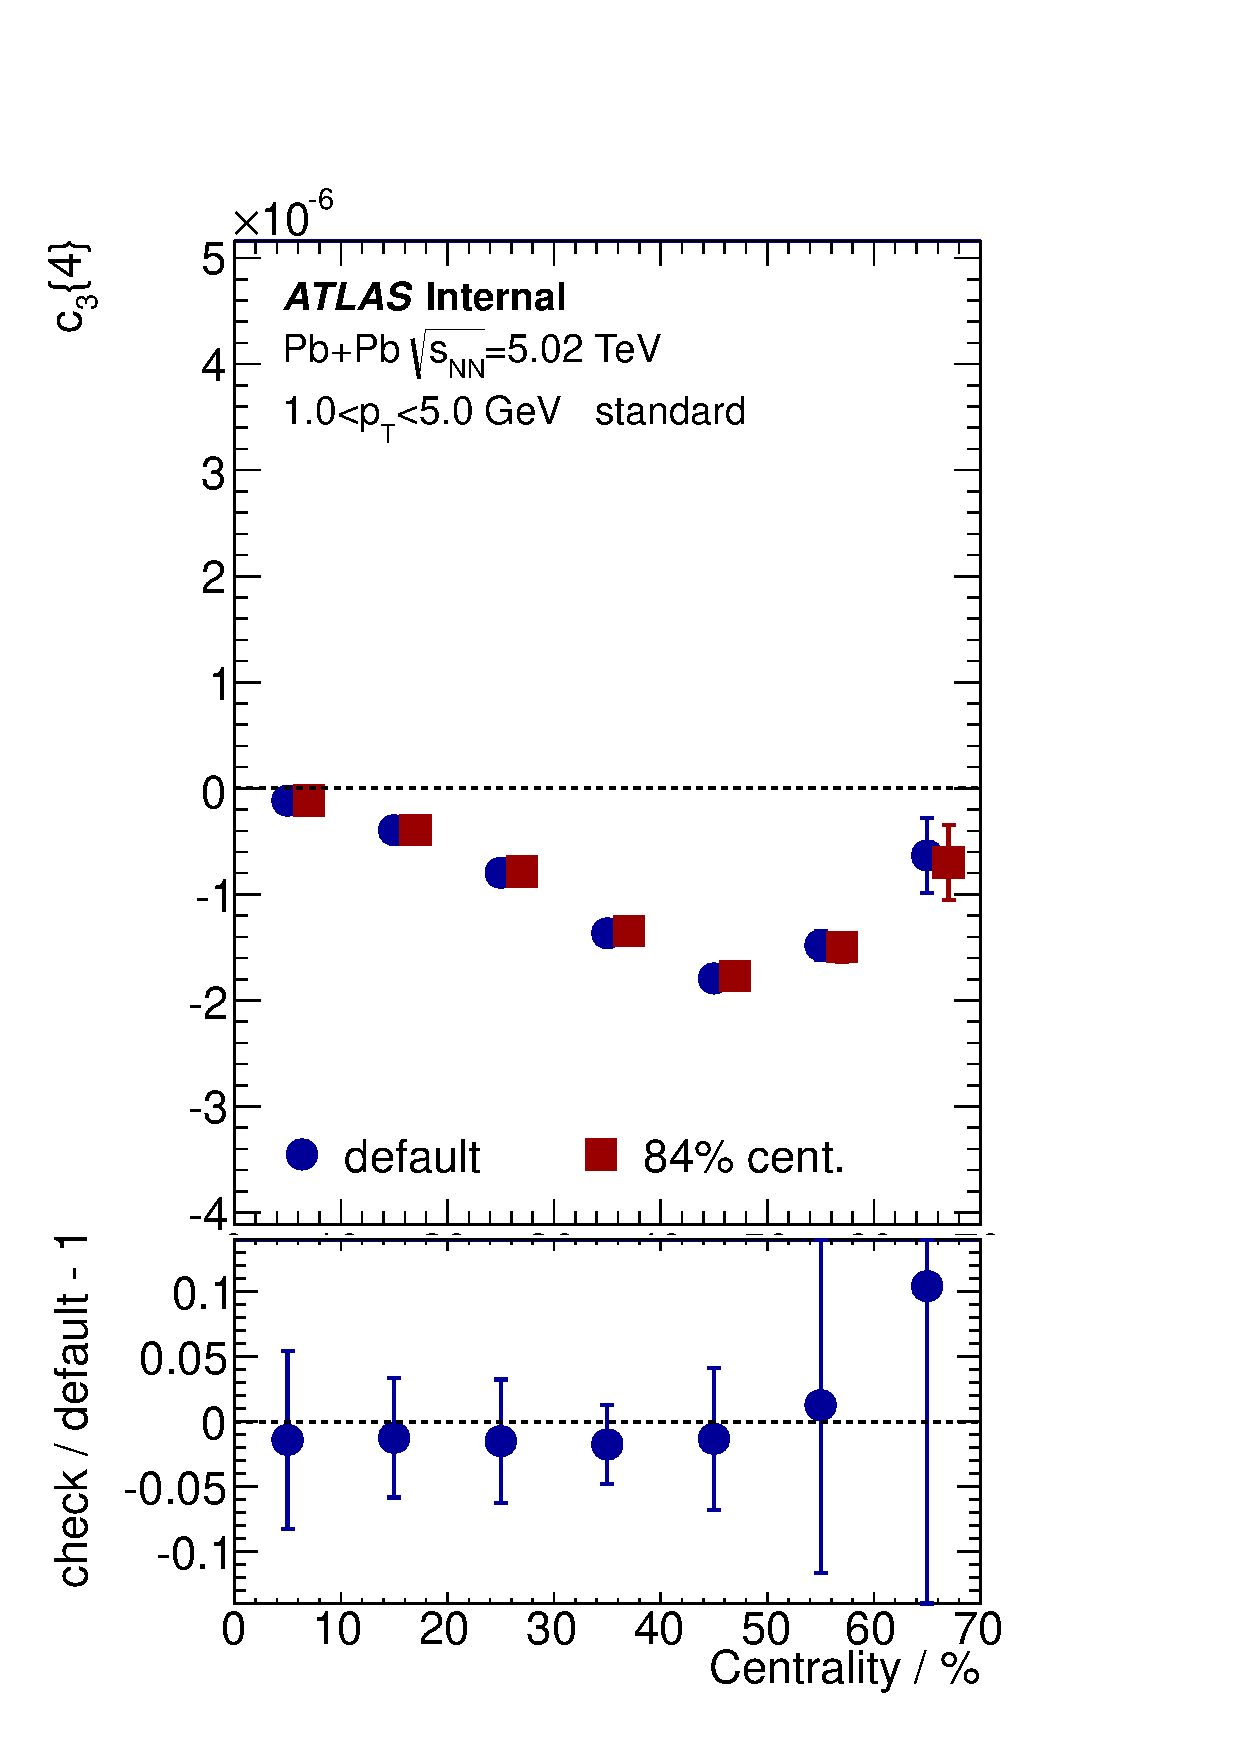
\includegraphics[width=.24\linewidth]{figs/chapter_appendix/centrality_Har3_Pt1.pdf}
\caption{Systematics of $c_n\{4\}$ from centrality definition: $(0-85)\%$ v.s. $(0-84)\%$ . Bottom panels are the relative uncertainties between the default and check.}
\label{fig:appendix_centrality}
\end{figure}



\subsubsection{Monte-Carlo closure}

The HIJING Monte Carlo simulations were used to evaluate the difference between multi-particle cumulants in Pb+Pb data calculated using the generated and reconstructed charged particles obtained using the same analysis method. In some analysis it is considered as a crosscheck, since it assesses the quality of tracking, which are separately accounted for in previous systematics. The argument for not accounting it as a systematic uncertainties also relies on the fact that MC generators do not properly describe the investigated particle correlations. However, in this analysis, we are conservative to include the Monte-Carlo closure as part of the systematics.

Four million HIJING events with flow after-burner implemented are used for the MC closure (more details in \verb|ATLHI-116|). Note that both tracking and FCal $\Et$ are different between generated (truth) and reconstructed events, but in order to only evaluate the impact from offline tracking reconstruction, reconstructed FCal $\Et$, should be used for binning in both generated and reconstructed. Otherwise the differences between generated and reconstructed FCal $\Et$ will convolute with the tracking reconstruction, and that is not the purpose of this systematic check. However, the Monte-Carlo samples are generated using fast MC simulation configurations, which creates discrepancy of Calorimeter $\Et$ between data and MC. Due to this reason, the closure test was first binned in $\Nchrec$, which is consistent with data, then mapped to the FCal $\lr{\Et}$ of data. In this case, the mismatch of FCal $\Et$ between data and MC plays little role. The procedure is similar as the Run 2 $v_n$ analysis~\cite{Burka:2151932}.

For the reconstructed tracks, it is not required to be associated with truth track, and both efficiency and fake rates are needed for the correction. Meanwhile, we do observe that the average of $\phi$ distribution is not very uniform in reconstructed tracks due to the simulation of detector effects, so flattening procedure is also applied in this Monte-Carlo check. In summary, all the corrections that has been applied in data analysis are also repeated with the Monte-Carlo test.

Fig.~\ref{fig:appendix_mc_c} shows the $c_n\{4\}$ calculated from generated and reconstructed particles. Since the HIJING sample has flow implemented, both $c_2\{4\}$ and $c_3\{4\}$ show similar centrality dependence as data: largest in mid-central and approaches $0$ in central and peripheral. The relative differences are largest in central: reaching $3\%$, even after the efficiency and fake corrections are applied to the reconstructed tracks. As to $c_1\{4\}$ and $c_4\{4\}$, the centrality dependence is very different compared with data and the statistical errors are quite large. Due to these reasons, relative differences for $c_1\{4\}$ and $c_4\{4\}$ are not quoted as part of the systematics.
\begin{figure}[H]
\centering
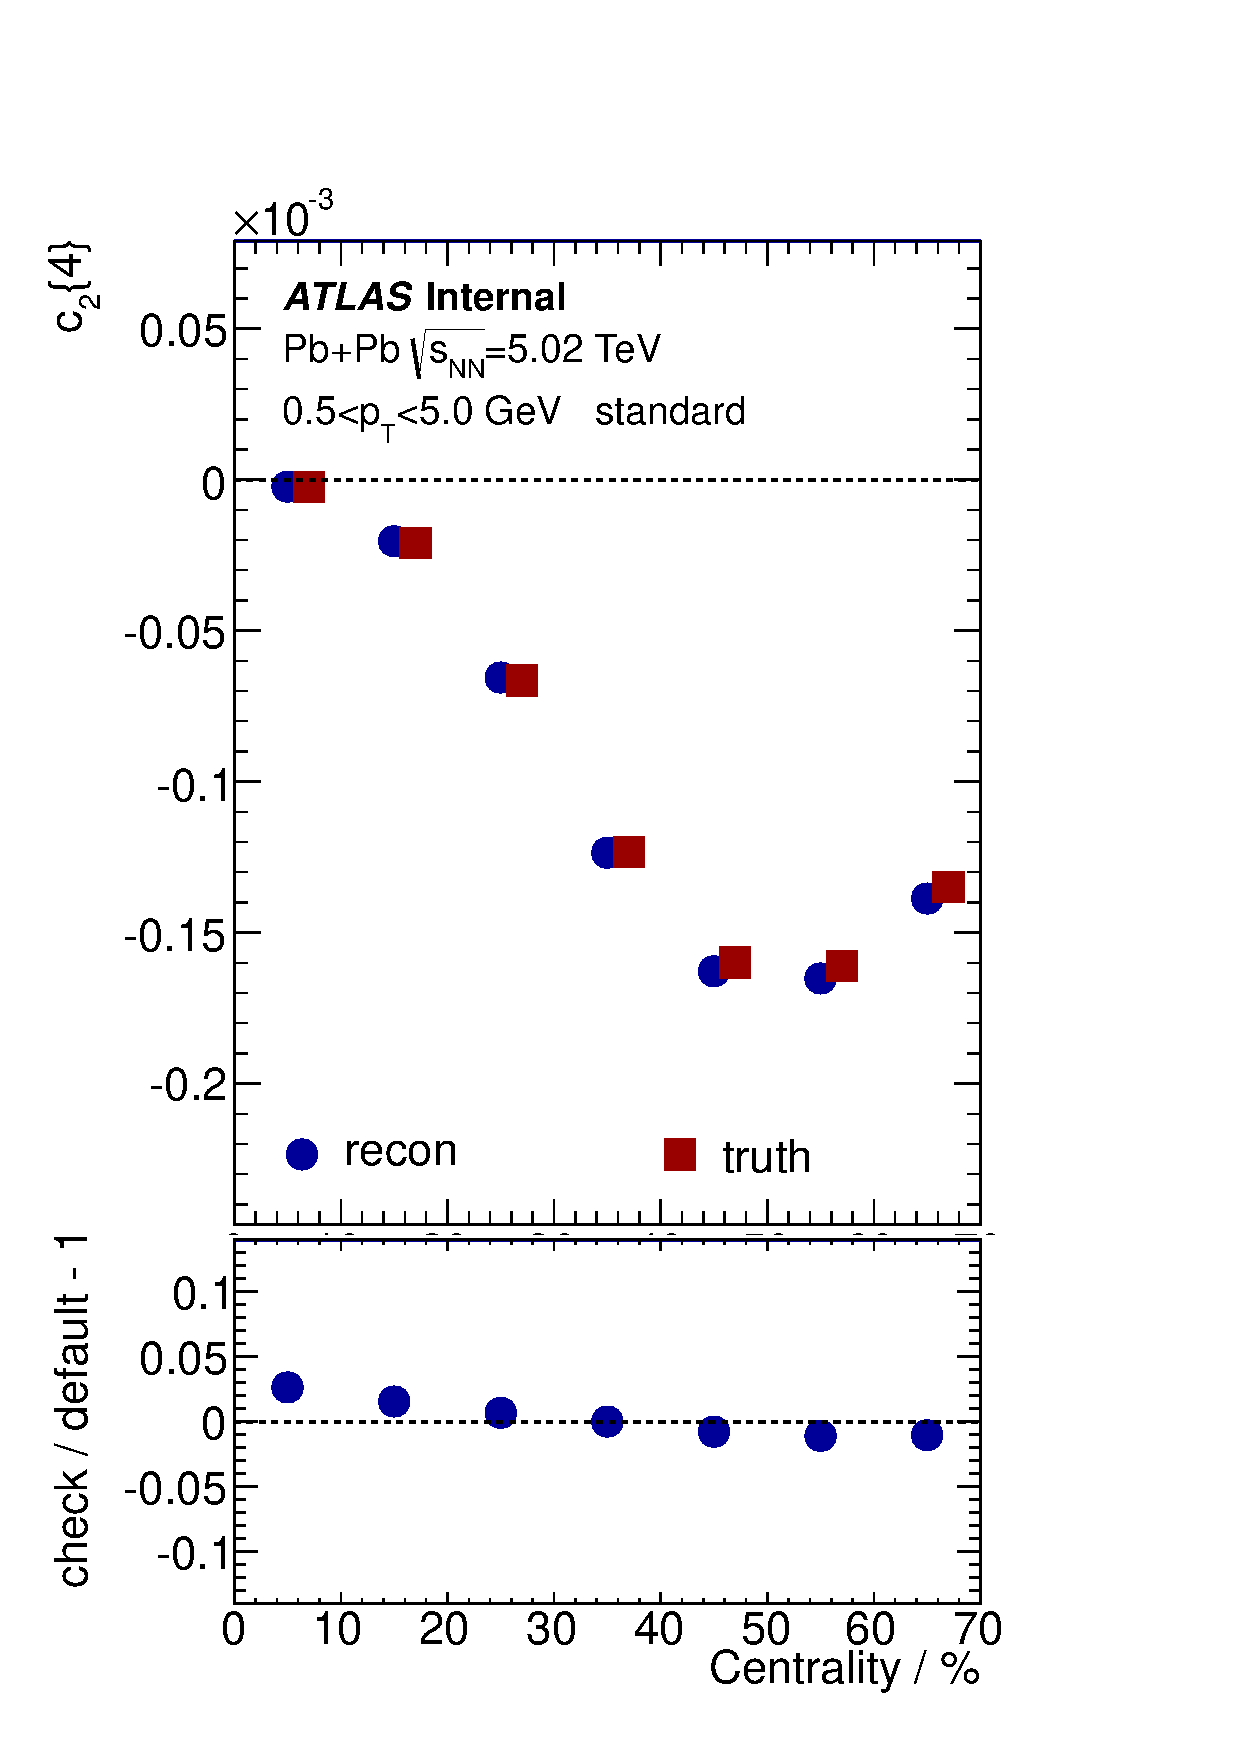
\includegraphics[width=.24\linewidth]{figs/chapter_appendix/mc_c_Har2_Pt0.pdf}
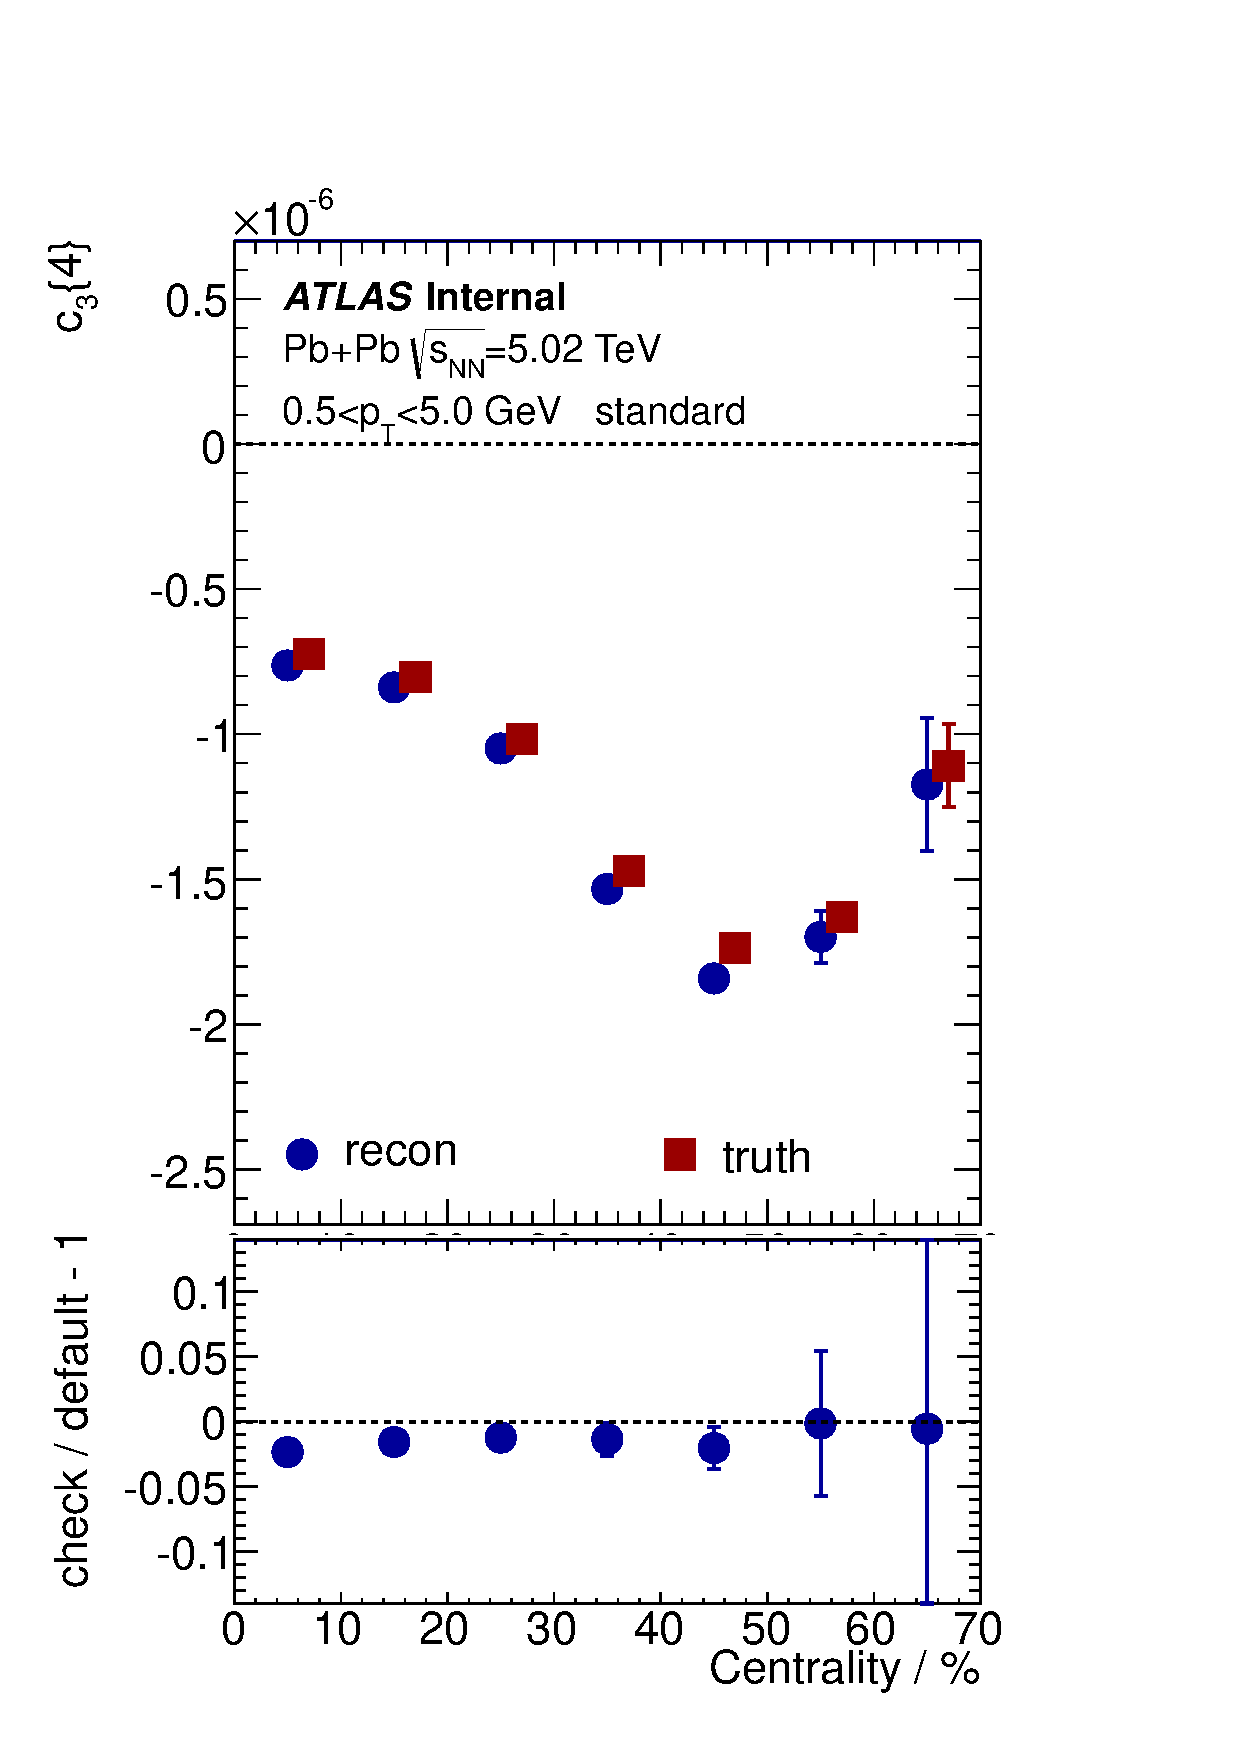
\includegraphics[width=.24\linewidth]{figs/chapter_appendix/mc_c_Har3_Pt0.pdf}
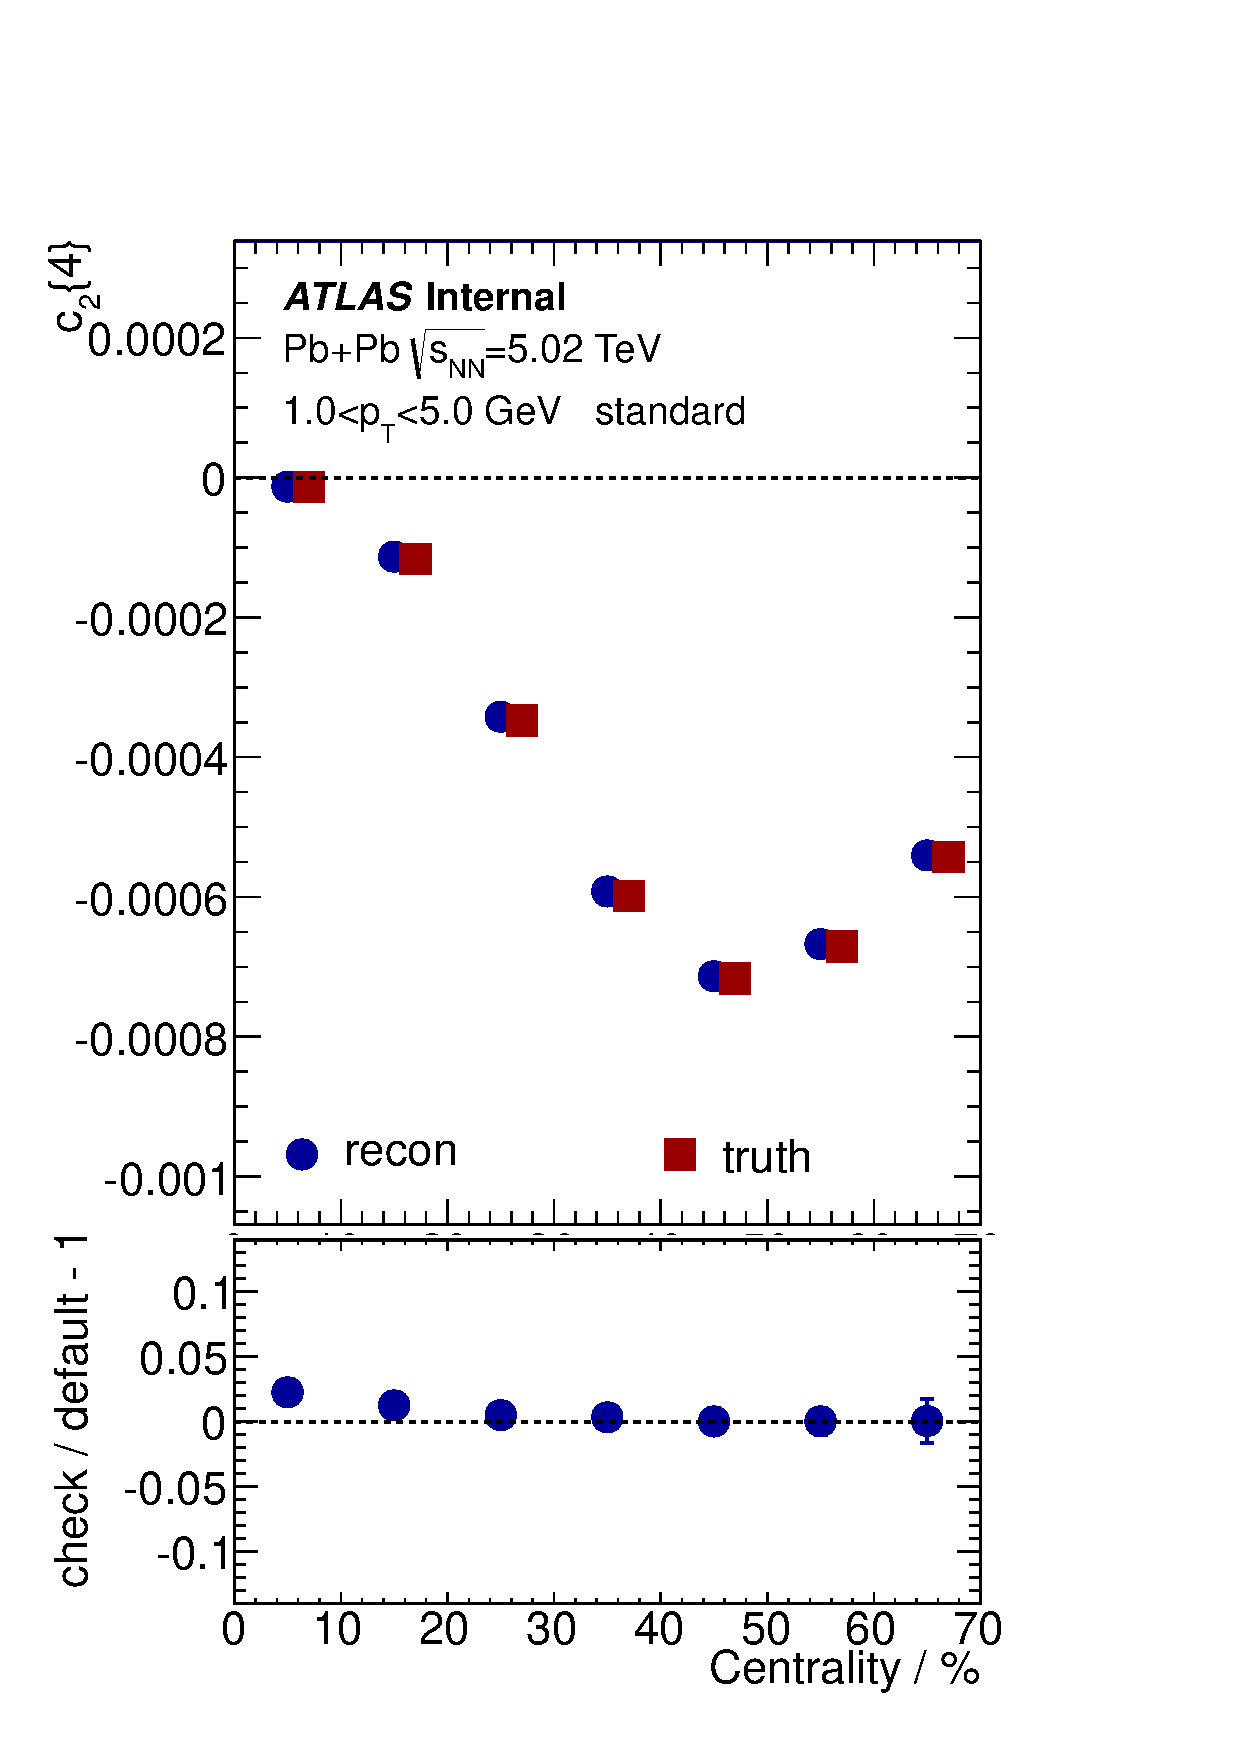
\includegraphics[width=.24\linewidth]{figs/chapter_appendix/mc_c_Har2_Pt1.pdf}
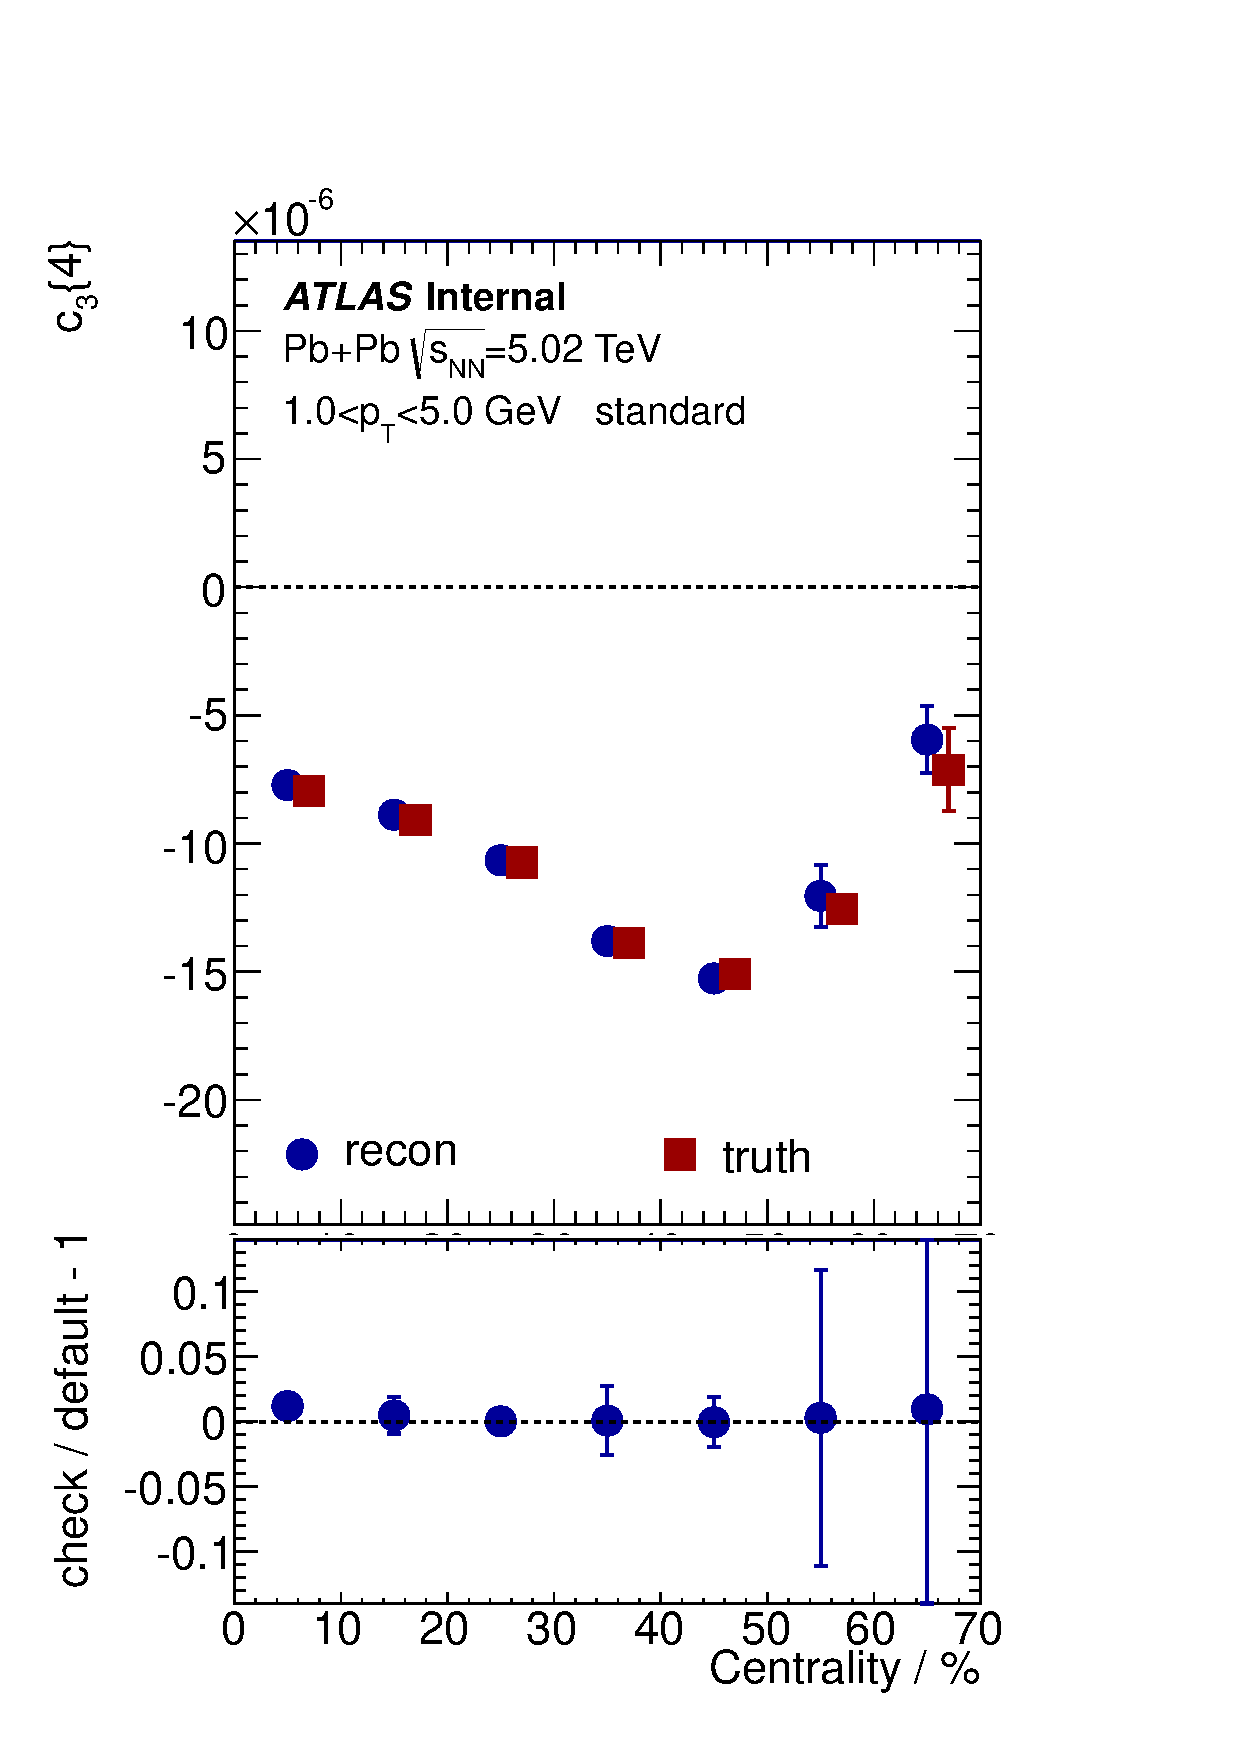
\includegraphics[width=.24\linewidth]{figs/chapter_appendix/mc_c_Har3_Pt1.pdf}
\caption{Systematics of $c_n\{4\}$ from MC closure: generated v.s. reconstructed. Bottom panels are the relative uncertainties between the default and check. Note that the relative difference for $c_1\{4\}$ and $c_4\{4\}$ are set to be 0 (see main text).}
\label{fig:appendix_mc_c}
\end{figure}

In addition, we have tested the following checks trying to diminish the $10\%$ differences observed in $c_2\{4\}$ and $c_3\{4\}$:
\begin{itemize}
\item Using a different 0.5 million HIJING sample (see in \verb|ATLHI-84|): similar outcome;
\item Do not apply efficiency or fake correction to reconstructed tracks: larger difference;
\item Only apply tracking efficiency: larger difference in central;
\item Apply flattening procedure on reconstructed tracks: similar outcome;
\item Apply additional $d_0$ and $z_0$ significance cuts to reconstructed tracks: larger difference;
\end{itemize}
Unfortunately, average efficiency and fake corrections will not compensate the inefficiency of reconstruction of tracks. To be conservative, the relative differences are quoted as systematics for both $c_2\{4\}$ and $c_3\{4\}$. As to the systematics in ultra-central collisions, since this HIJING sample does not contain enough ultra-central events, the systematic errors in UCC events are quoted from the plots above (error from the most central bin).

Since HIJING simulation does not implement correlation between flow harmonics, as shown in Fig.~\ref{fig:appendix_mc_sc}(the signals are much smaller compared with data), systematics from MC closure for symmetric and asymmetric cumulant are set to be zero.
\begin{figure}[H]
\centering
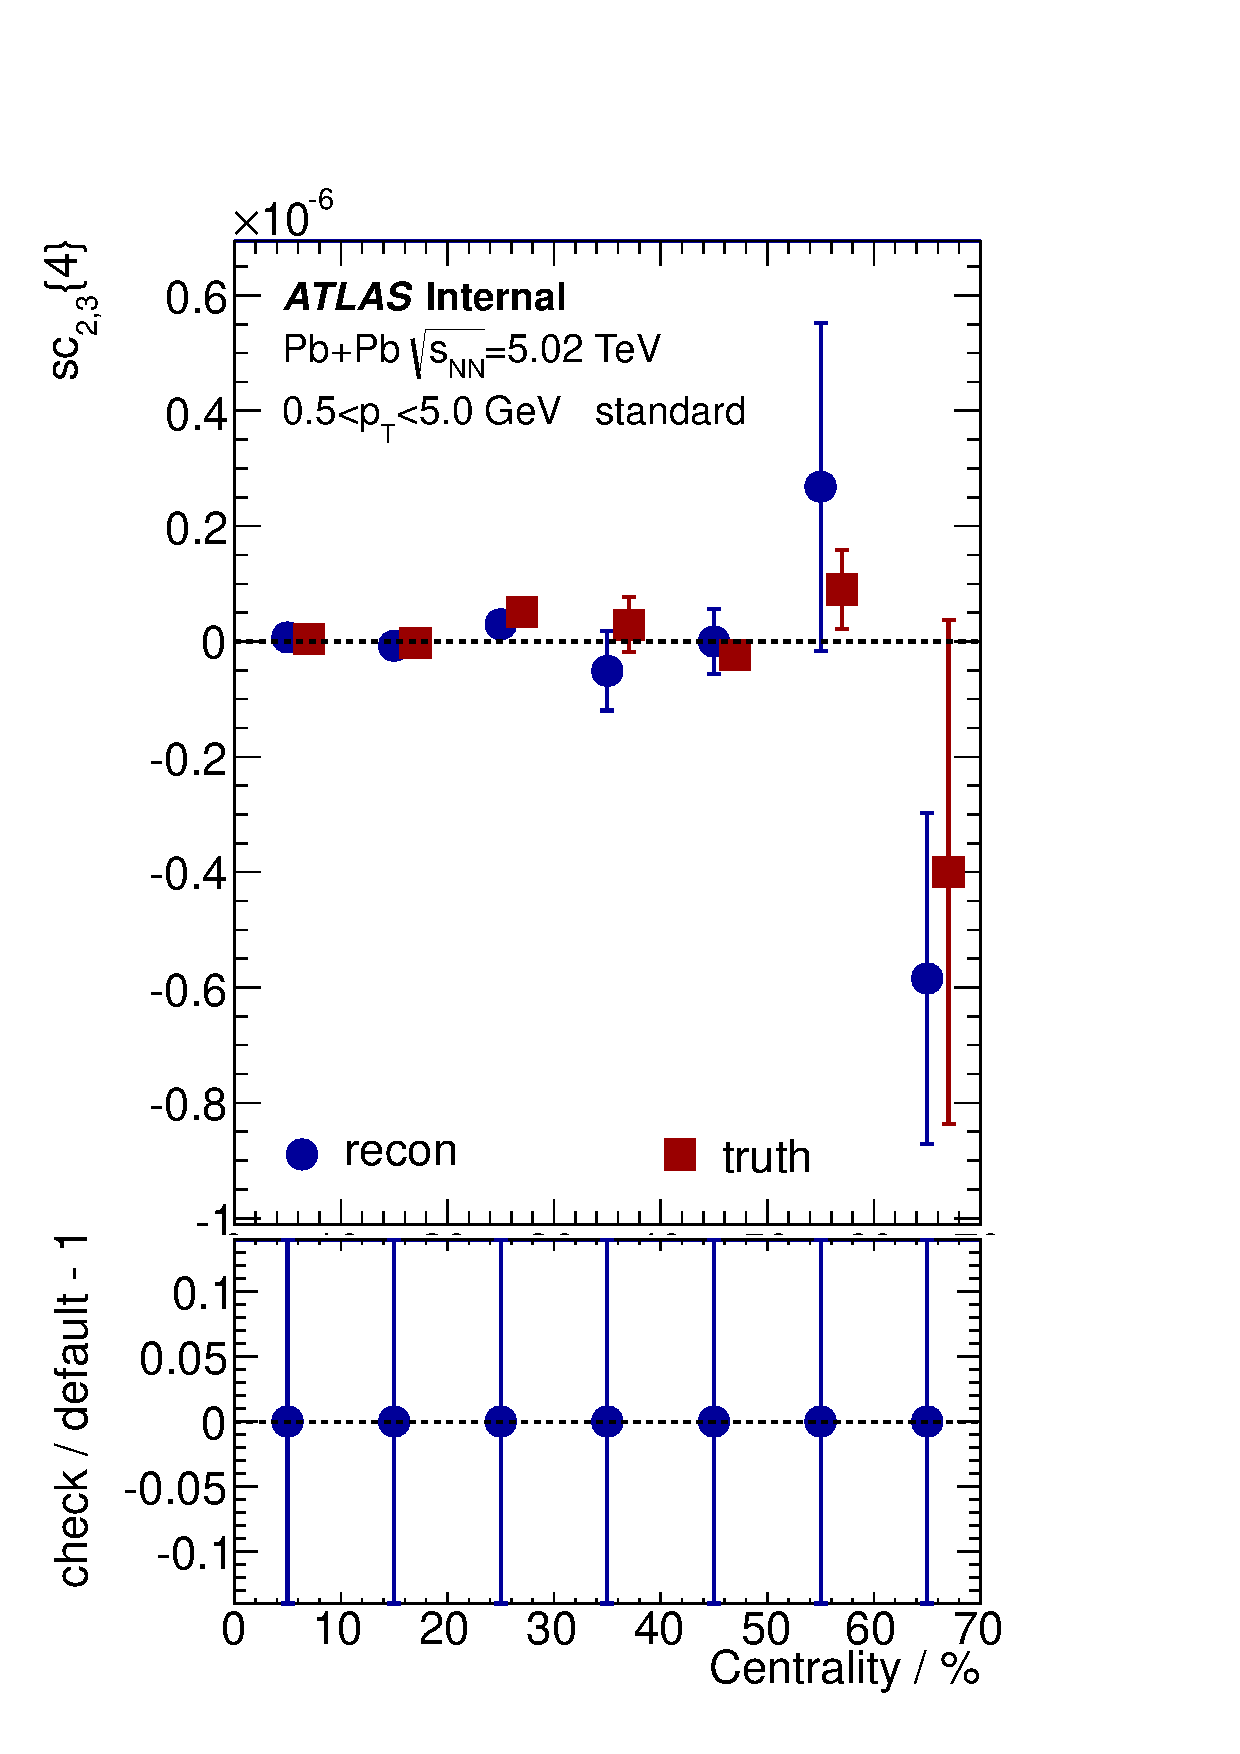
\includegraphics[width=.24\linewidth]{figs/chapter_appendix/mc_sc_Har2_Pt0.pdf}
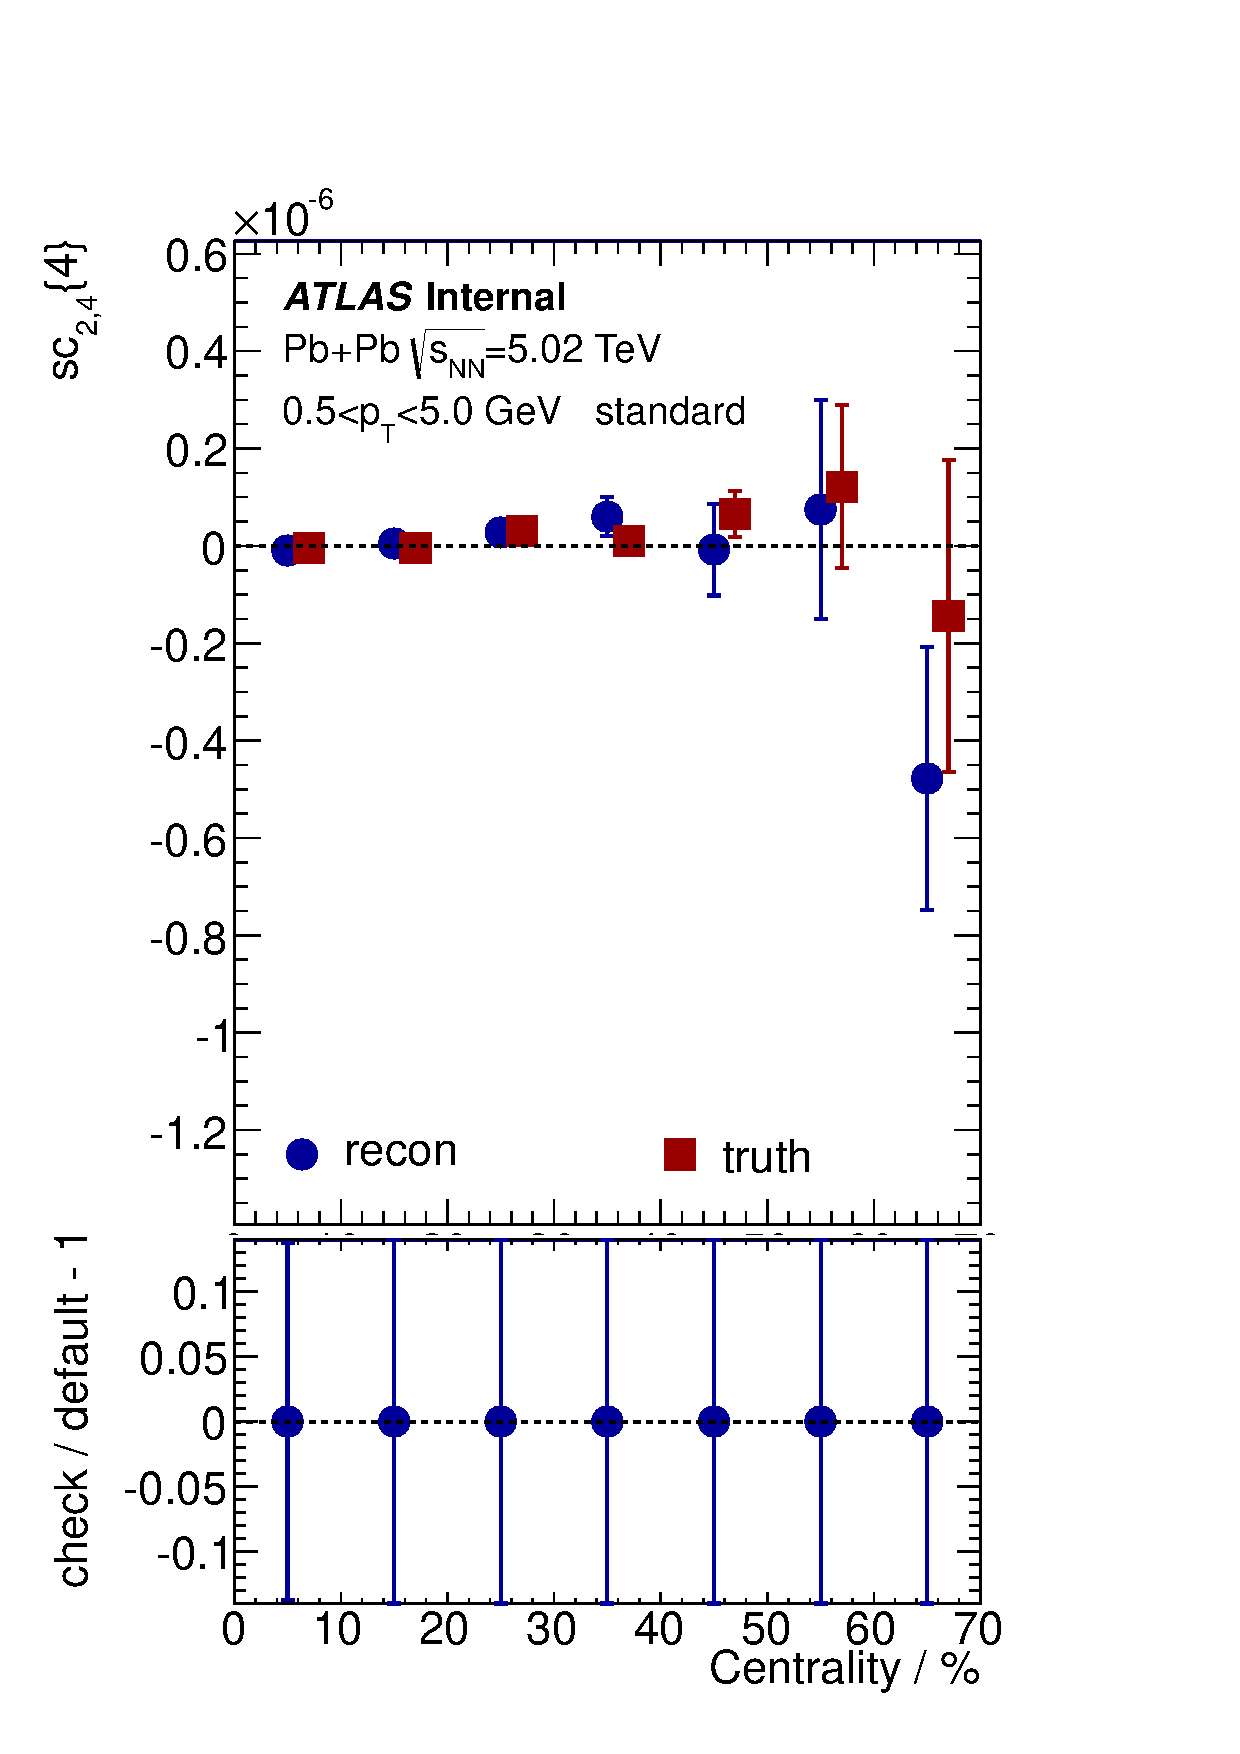
\includegraphics[width=.24\linewidth]{figs/chapter_appendix/mc_sc_Har3_Pt0.pdf}
\caption{Systematics of symmetric cumulants from MC closure: generated v.s. reconstructed. Bottom panels are the relative uncertainties between the default and check. Note that the relative differences are set to be zero (see main text).}
\label{fig:appendix_mc_sc}
\end{figure}




\subsubsection{Flattening}

Tracking efficiency weighting corrects the possible detector effects as a function of $\eta$ and $\pT$ , but the residual detector effects could still remain in the $\phi$ direction. In heavy ion collision, since the ”event plane” angle is random from event to event, the $\phi$ distribution averaged over many events should be flat and the discrepancy is due to the detector effects.

To estimate the impact from detector effects, the flattening produce was performed. The correction factor, $w_\phi$, is defined as:
\begin{equation}
w_\phi(\eta,\phi)\equiv\frac{\lr{N(\delta\eta)}}{N(\delta\eta,\delta\phi)}
\end{equation}
where $N(\delta\eta,\delta\phi)$ is the number of particles in the small $(\eta,\phi)$ phase-space window; and $\lr{N(\delta\eta)}$ is the mean number of particles in the small $\eta$ slice averaged over the whole $\phi$ range. $w_\phi$ is evaluated run-by-run, as a function of $\pT$, vertex position $z_{vtx}$ and charge, so that it can properly correct the detector effects.

To illustrate how the flattening works, Fig.~\ref{fig:appendix_flatten_eg} shows the $\eta-\phi$ distributions before (left) and after (right) flattening. Several holes are observed in the raw $\eta-\phi$ distribution, while after flattening, the average $\phi$ distribution is flat by construction in each $\eta$ slice.
\begin{figure}[H]
\centering
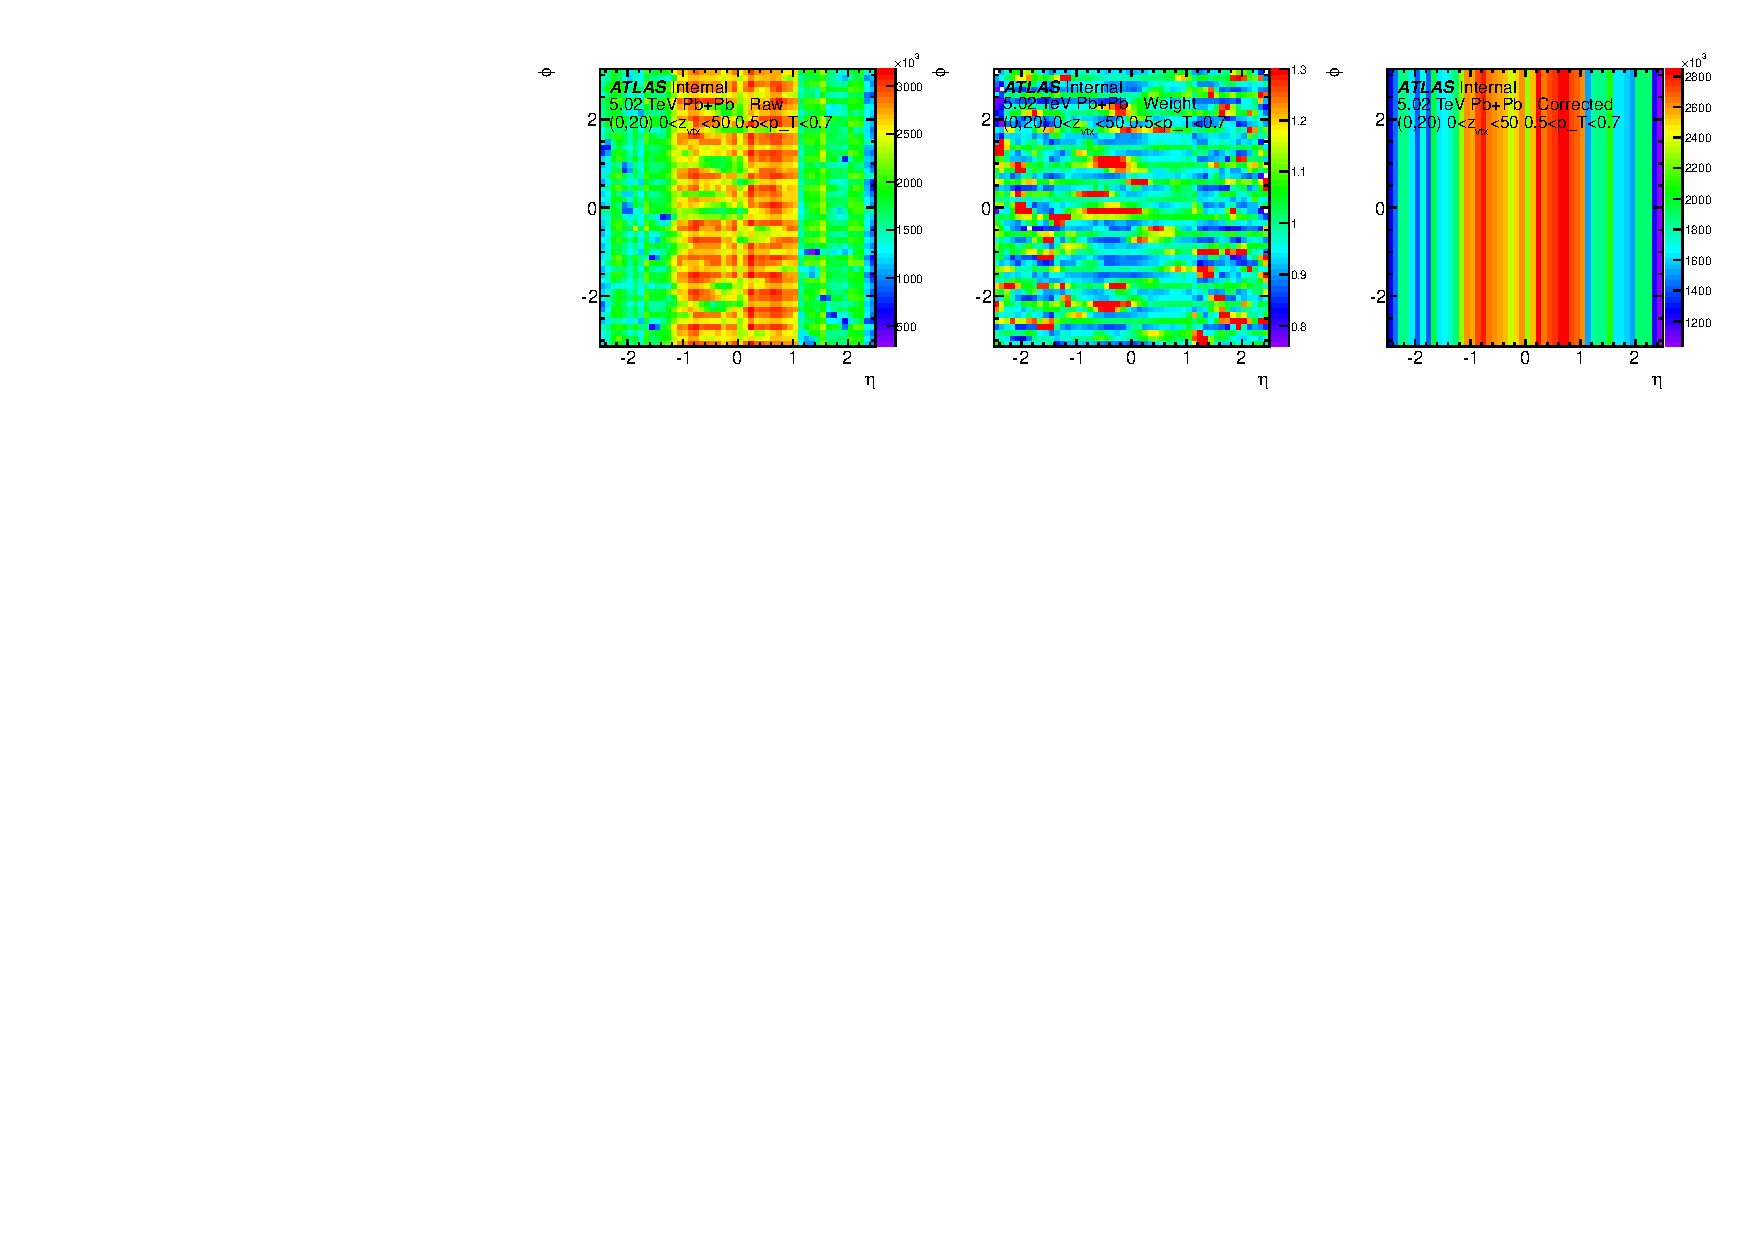
\includegraphics[width=1.\linewidth]{figs/chapter_appendix/flatten_eg.pdf}
\caption{An example demonstrating how flattening works. Left plot is the raw $\eta-\phi$ distribution, while right plot is the $\eta-\phi$ distribution after flattening procedure. Middle panel shows the correction factor $w_\phi$.}
\label{fig:appendix_flatten_eg}
\end{figure}

A comparison of $c_n\{4\}$ before and after flattening is shown in Fig.~\ref{fig:appendix_flatten1}. For all the harmonics, the relative differences are within $10\%$ and within statistical uncertainties. However, the relative difference seems to increase towards the central collision. Since the detector effect indeed depends on the occupancy of detector, it is worth checking the impact from flattening in UCC in details.
\begin{figure}[H]
\centering
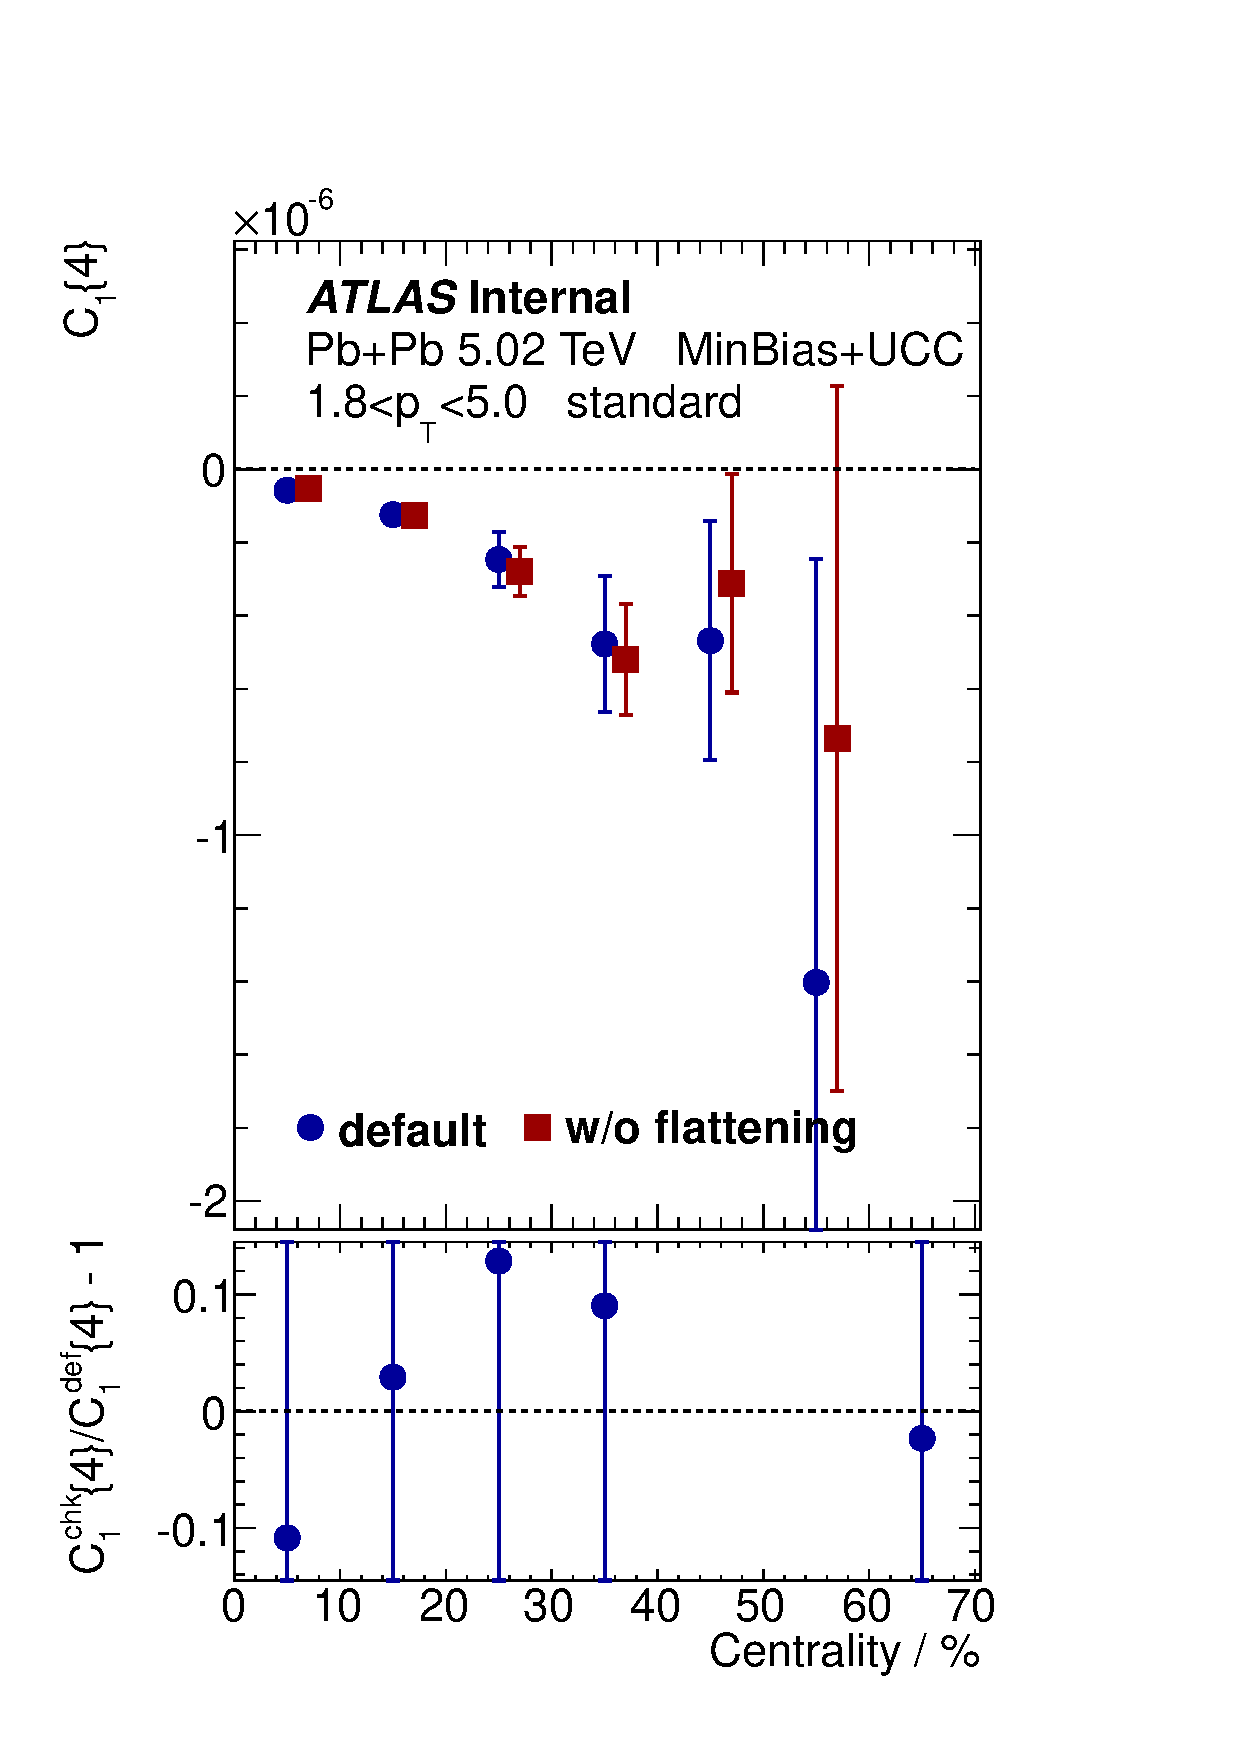
\includegraphics[width=.24\linewidth]{figs/chapter_appendix/flatten1_Har1.pdf}
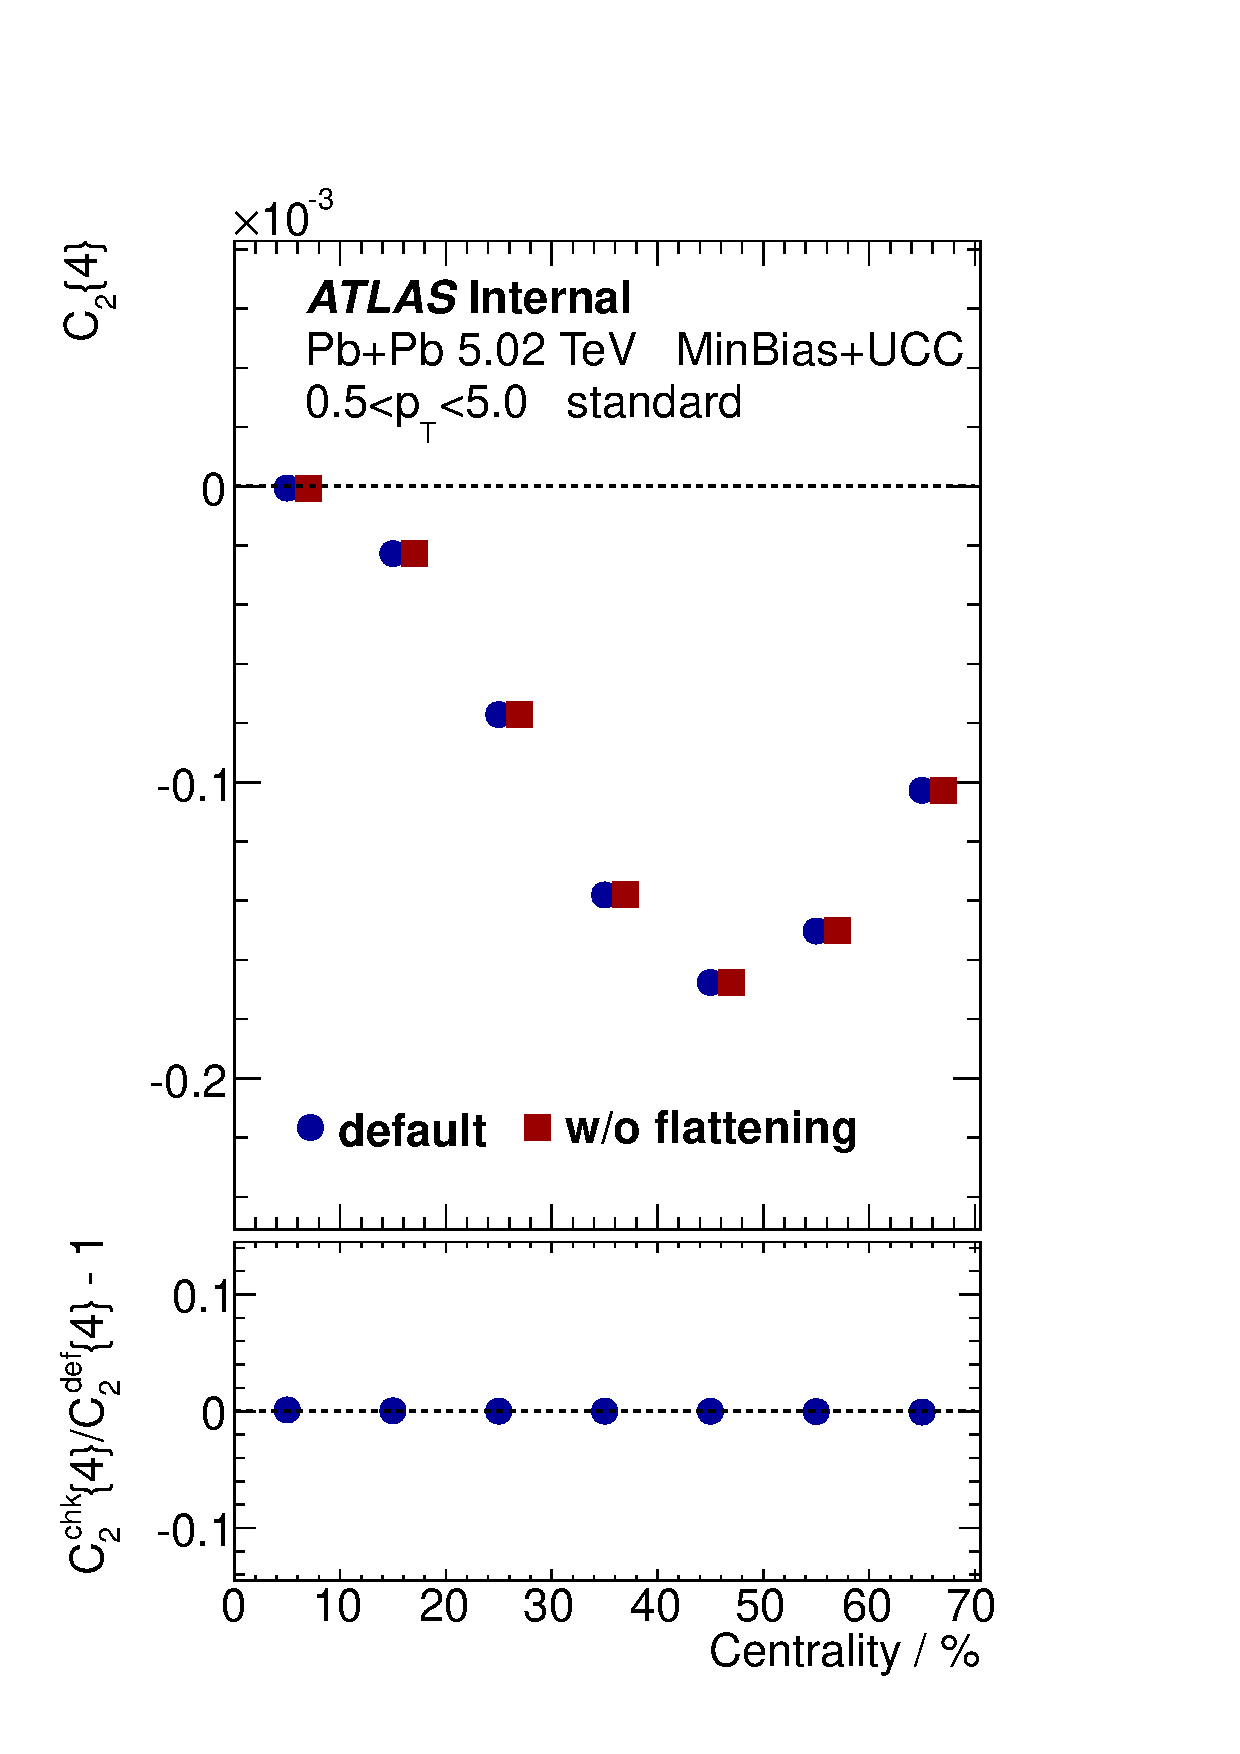
\includegraphics[width=.24\linewidth]{figs/chapter_appendix/flatten1_Har2.pdf}
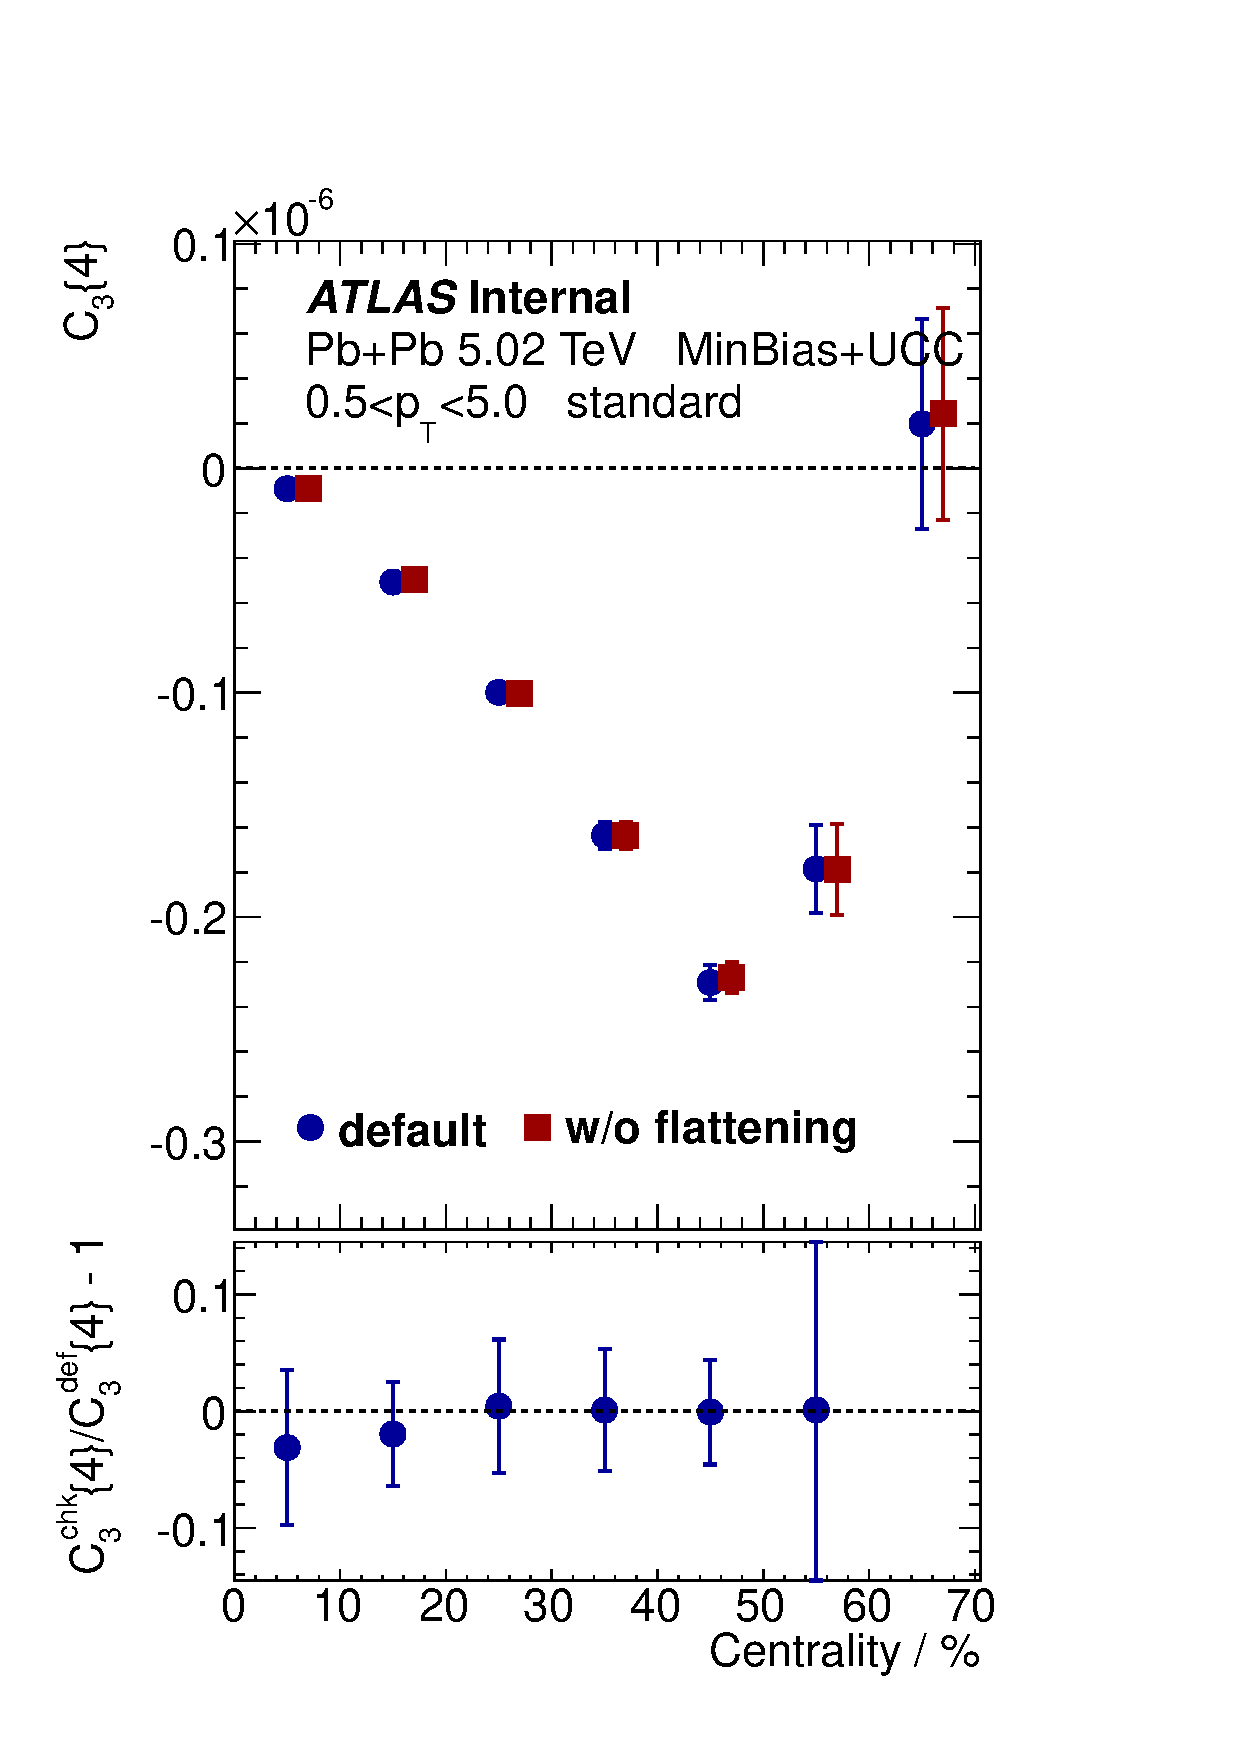
\includegraphics[width=.24\linewidth]{figs/chapter_appendix/flatten1_Har3.pdf}
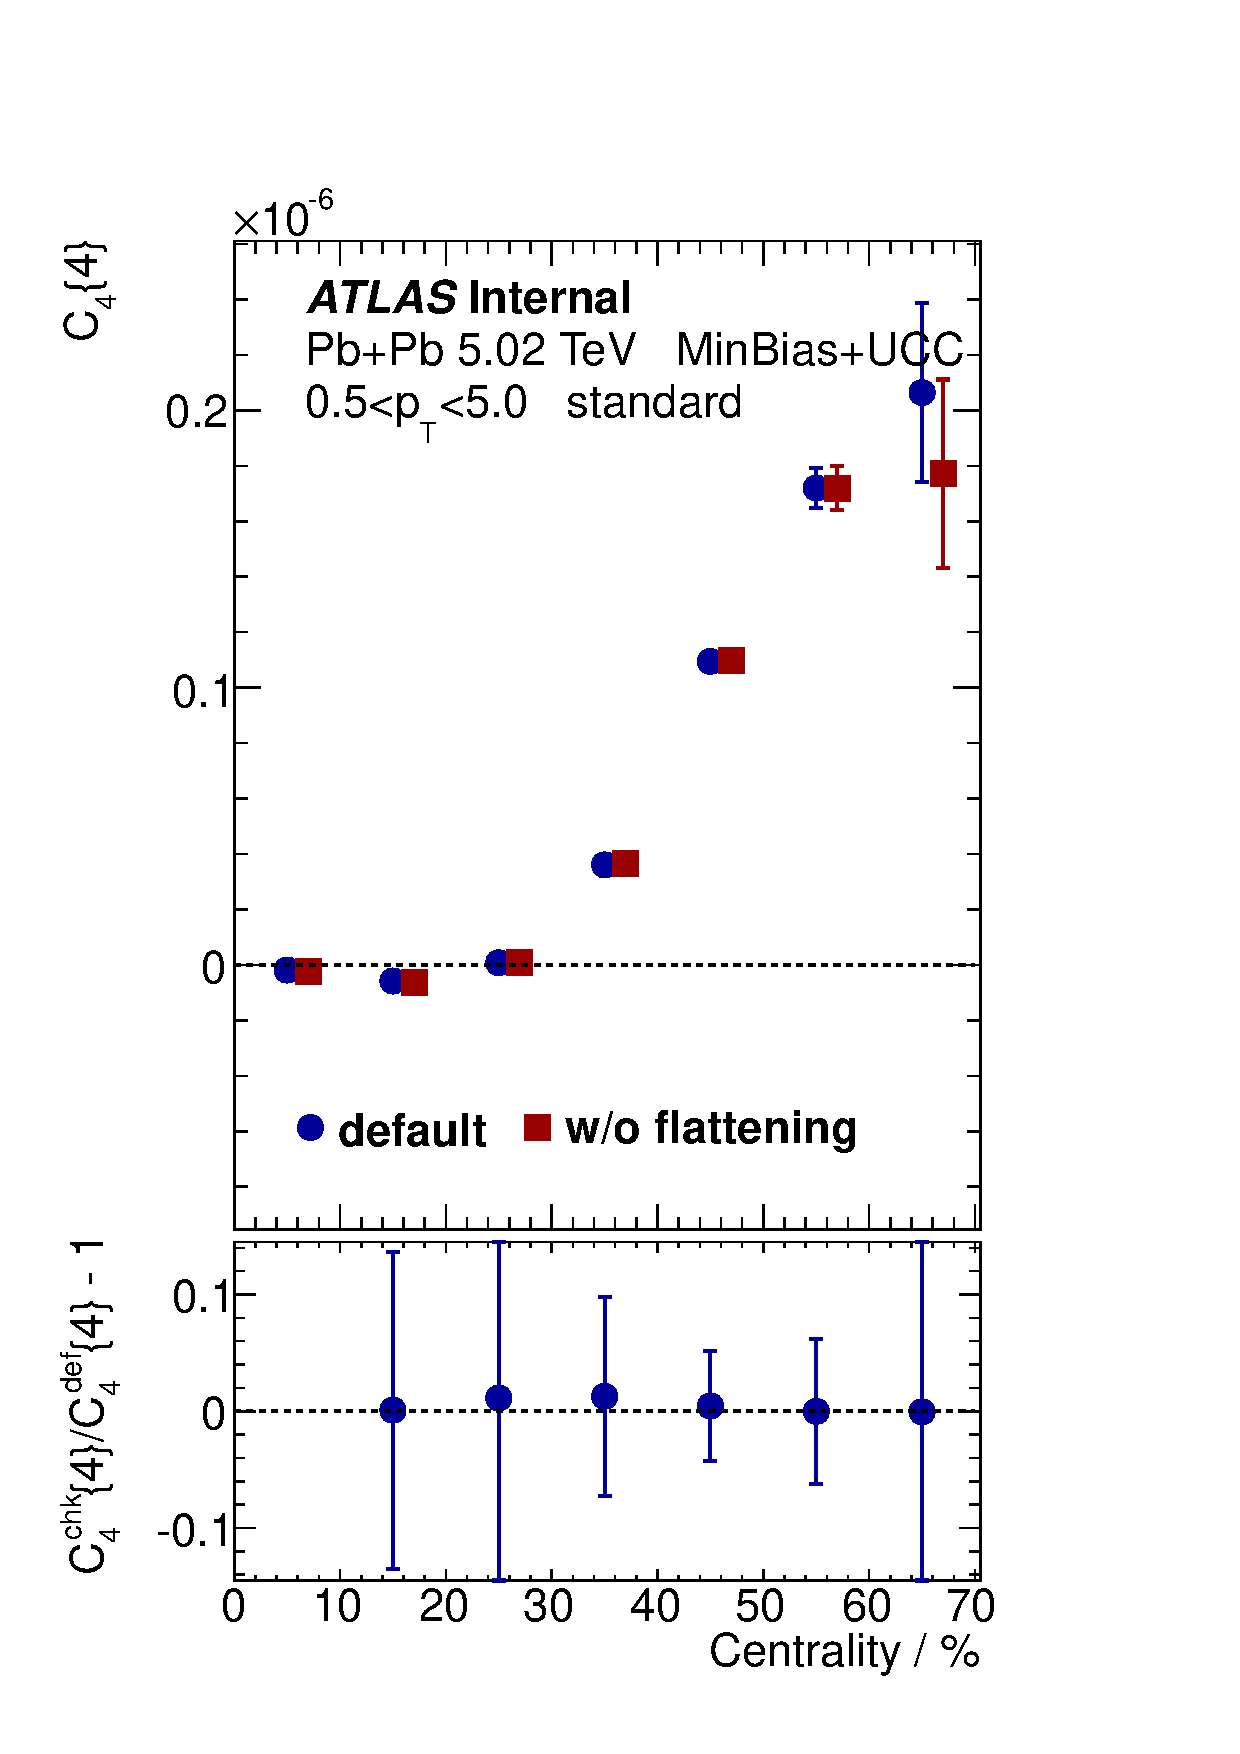
\includegraphics[width=.24\linewidth]{figs/chapter_appendix/flatten1_Har4.pdf}
\caption{Systematics of $c_n\{4\}$ from flattening procedure: with and without flattening. Bottom panels are the relative uncertainties between the default and check.}
\label{fig:appendix_flatten1}
\end{figure}

A comparison of $c_n\{4\}$ in ultra-central collisions before and after flattening is shown in Fig.~\ref{fig:appendix_flatten2}. For the odd harmonics $c_1\{4\}$ and $c_3\{4\}$, flattening does not change the results too much: the relative differences are within $10\%$ and still within statistical errors. However, for the even harmonics, especially for $c_2\{4\}$, the positive magnitude without flattening is smaller than default. Since the flattening is an essential procedure to account for the detector effects. This check will be quoted as the systematics.
\begin{figure}[H]
\centering
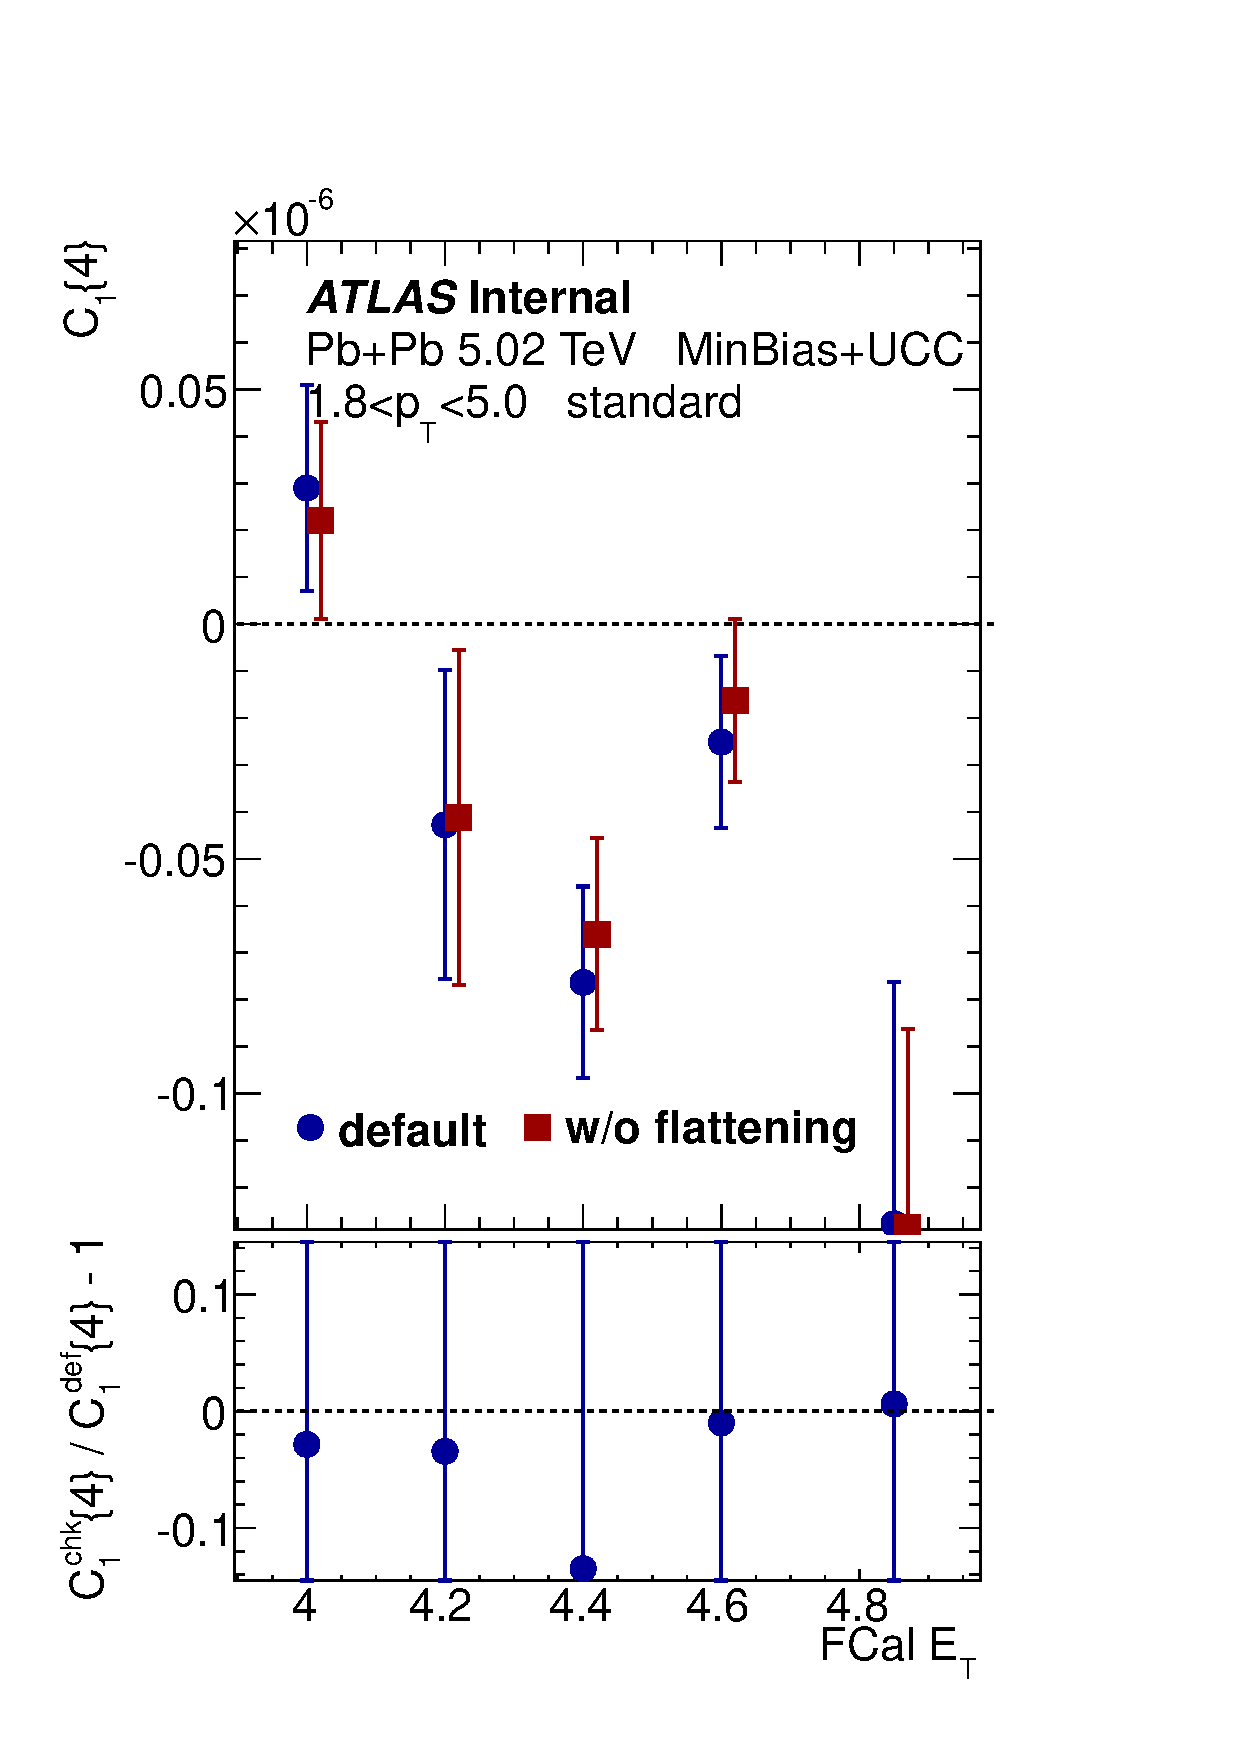
\includegraphics[width=.24\linewidth]{figs/chapter_appendix/flatten2_Har1.pdf}
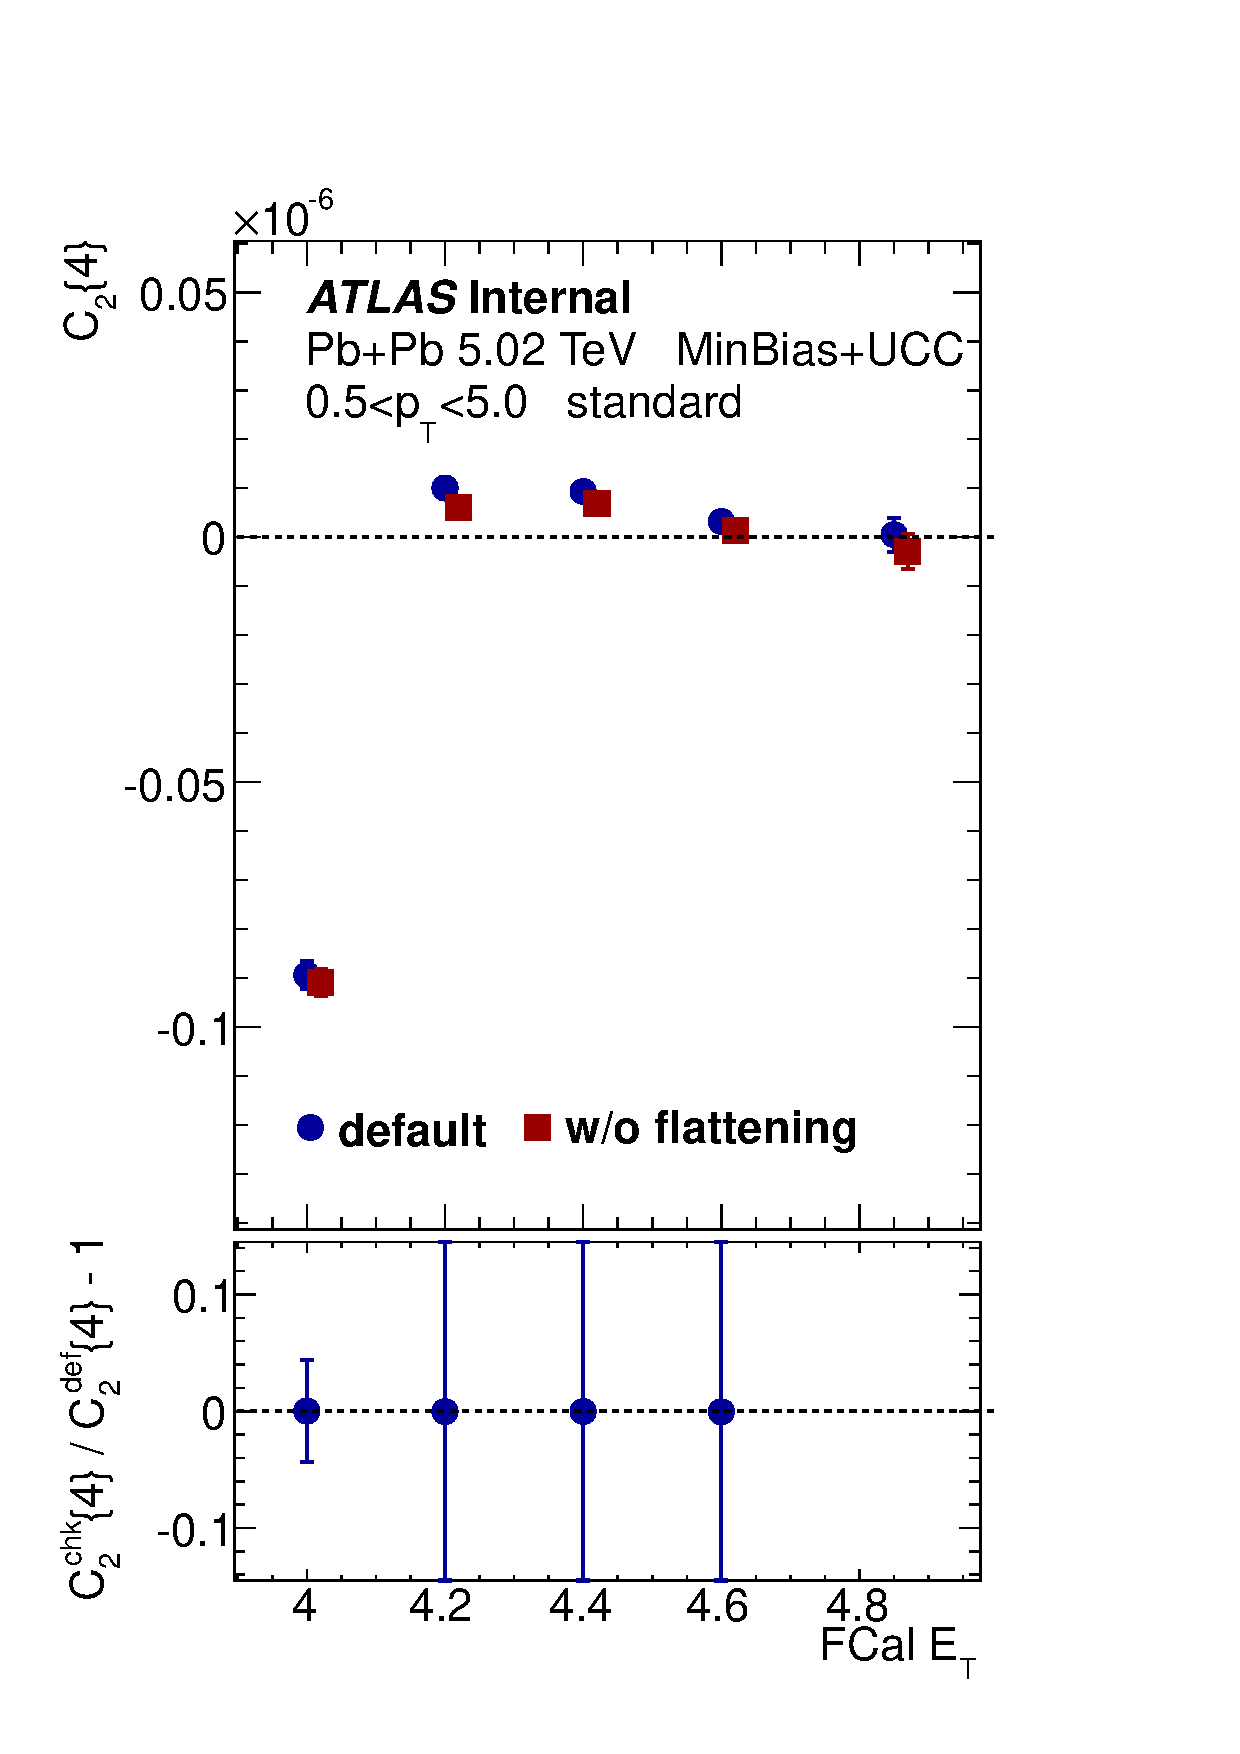
\includegraphics[width=.24\linewidth]{figs/chapter_appendix/flatten2_Har2.pdf}
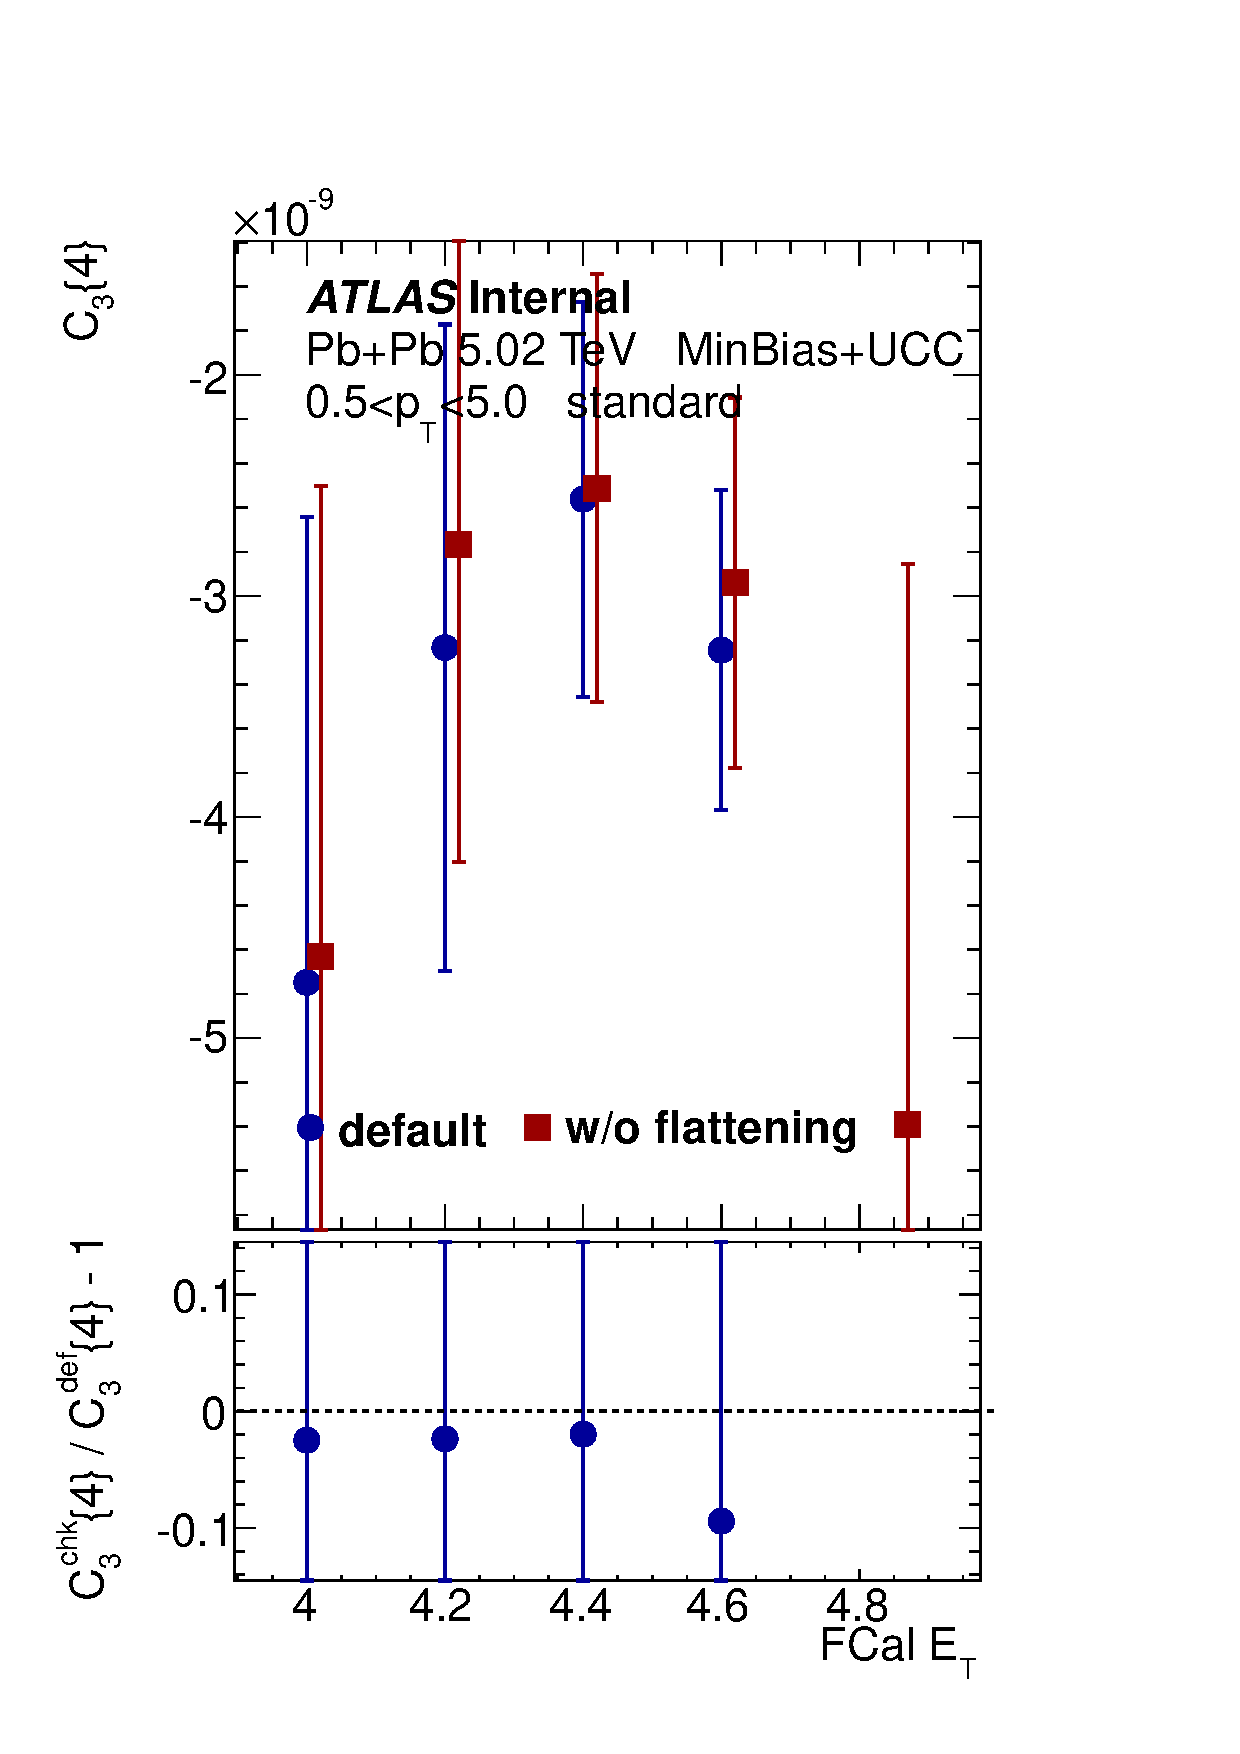
\includegraphics[width=.24\linewidth]{figs/chapter_appendix/flatten2_Har3.pdf}
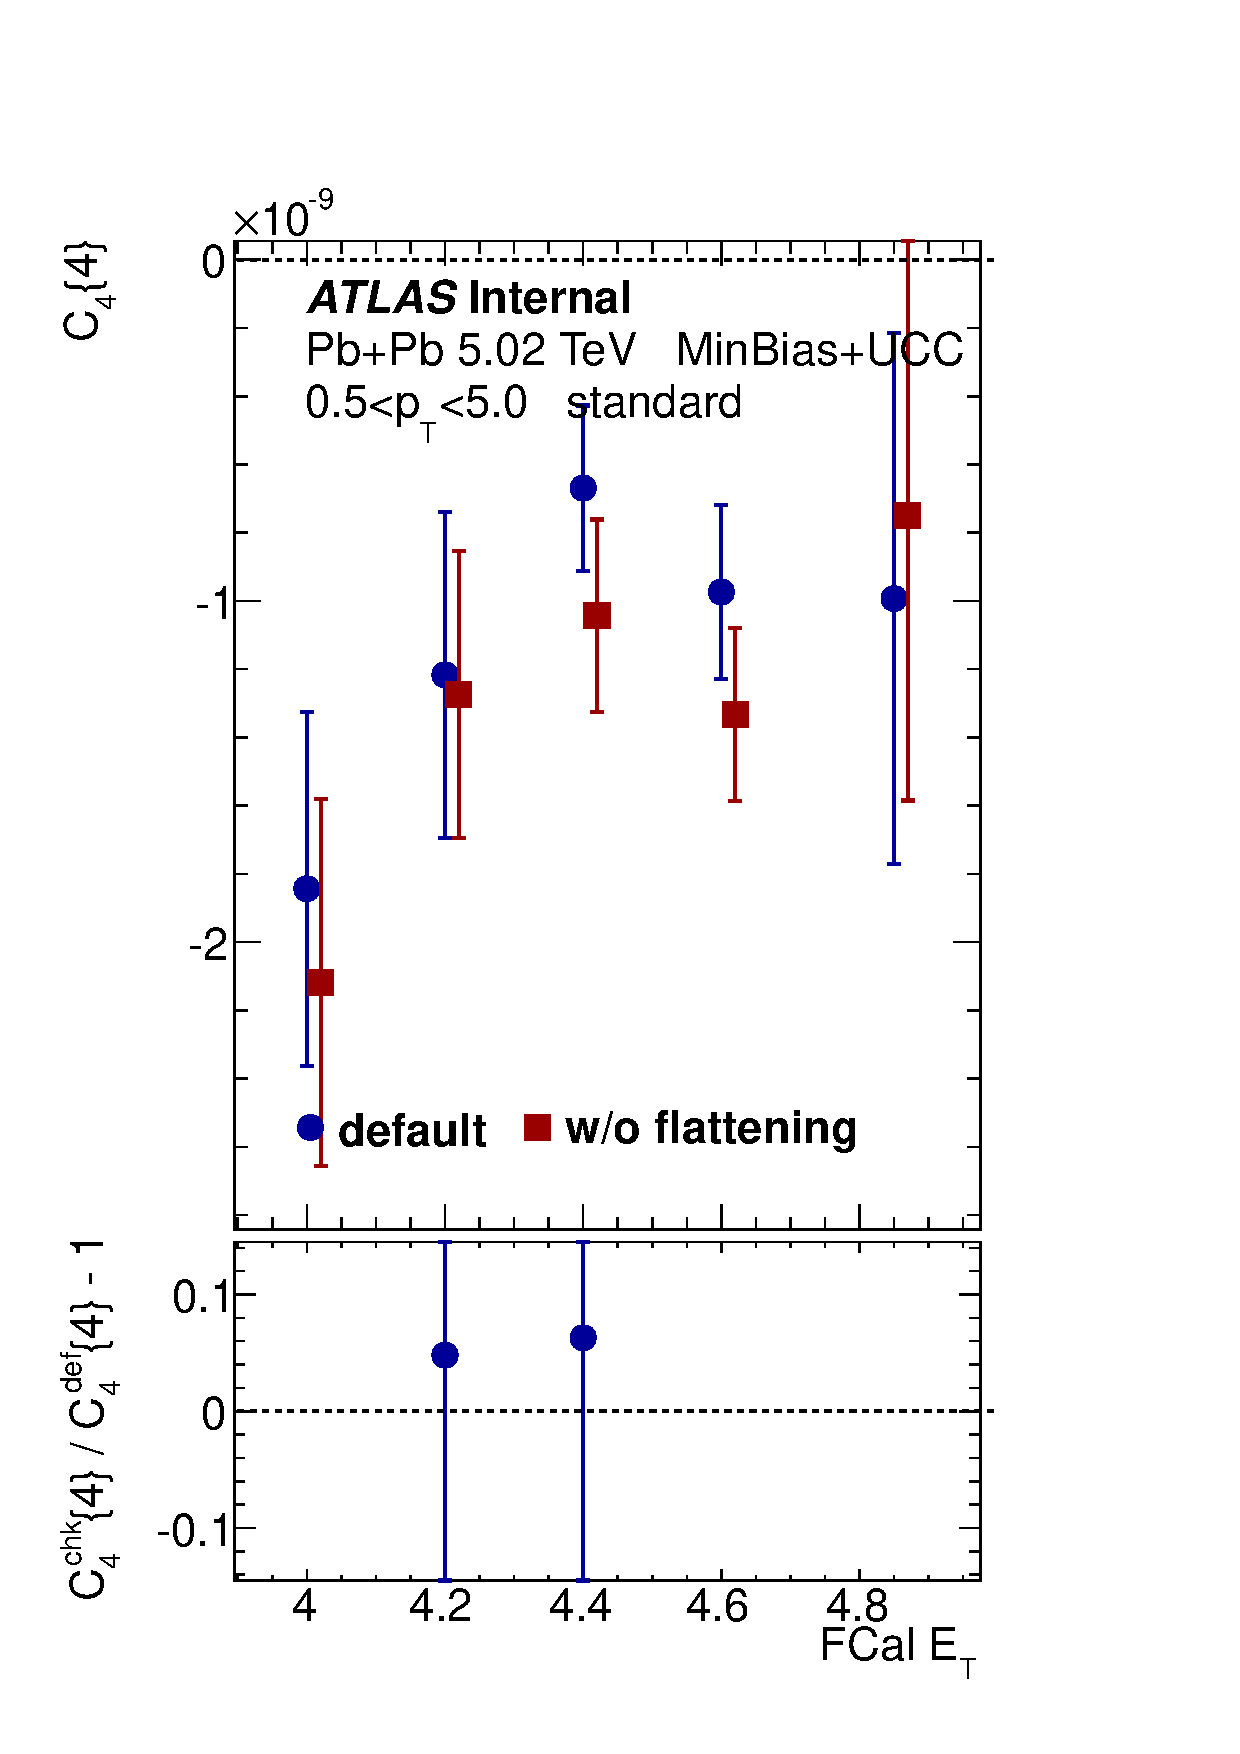
\includegraphics[width=.24\linewidth]{figs/chapter_appendix/flatten2_Har4.pdf}
\caption{Systematics of $c_n\{4\}$ in ultra-central collisions from flattening procedure: with and without flattening. Bottom panels are the relative uncertainties between the default and check.}
\label{fig:appendix_flatten2}
\end{figure}



\subsubsection{Track selection}
\label{sec:track_selection}

As default, the heavy ion loose track quality cut is applied in this analysis. In order to check stability of the track selection cuts, analysis is also repeated with tight track quality cut:
\begin{itemize}
\item Default: HI loose quality cut;
\item Check: HI tight quality cut;
\end{itemize}
where the definitions of loose and tight are listed in data selection section.

Fig.~\ref{fig:appendix_trkSel} compares the $c_n\{4\}$ calculated with HI loose and tight track selection. For $c_2\{4\}$ and $c_3\{4\}$, the relative differences are within $3\%$ for all centralities. While for $c_1\{4\}$ and $c_4\{4\}$, since the signal is much smaller, the relative errors go up to $10\%$, but still within statistical uncertainties. This is not surprising because even though different track selections give different fake rates, they are already corrected using Monte-Carlo. Systematics from track selection are quoted as part of the combined systematics, for all the harmonics.
\begin{figure}[H]
\centering
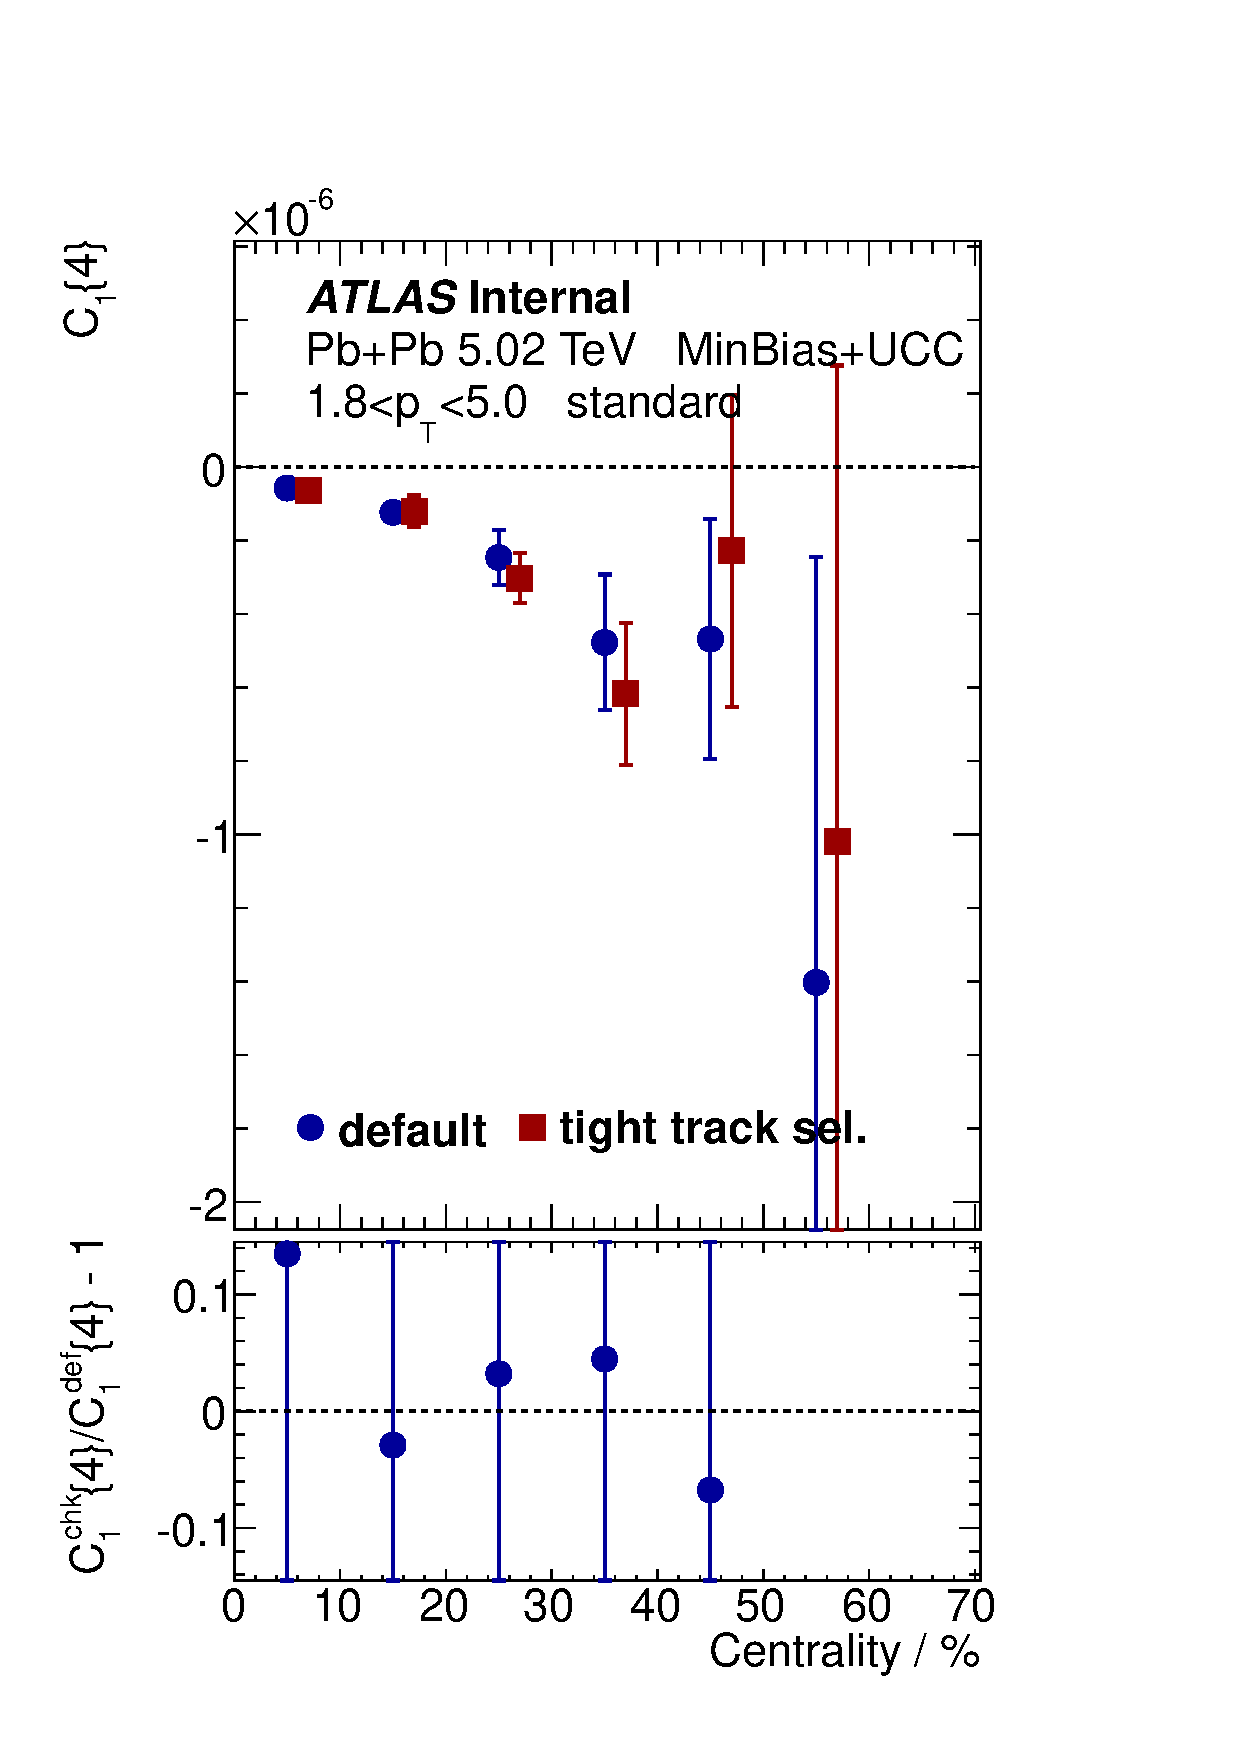
\includegraphics[width=.24\linewidth]{figs/chapter_appendix/trkSel_Har1.pdf}
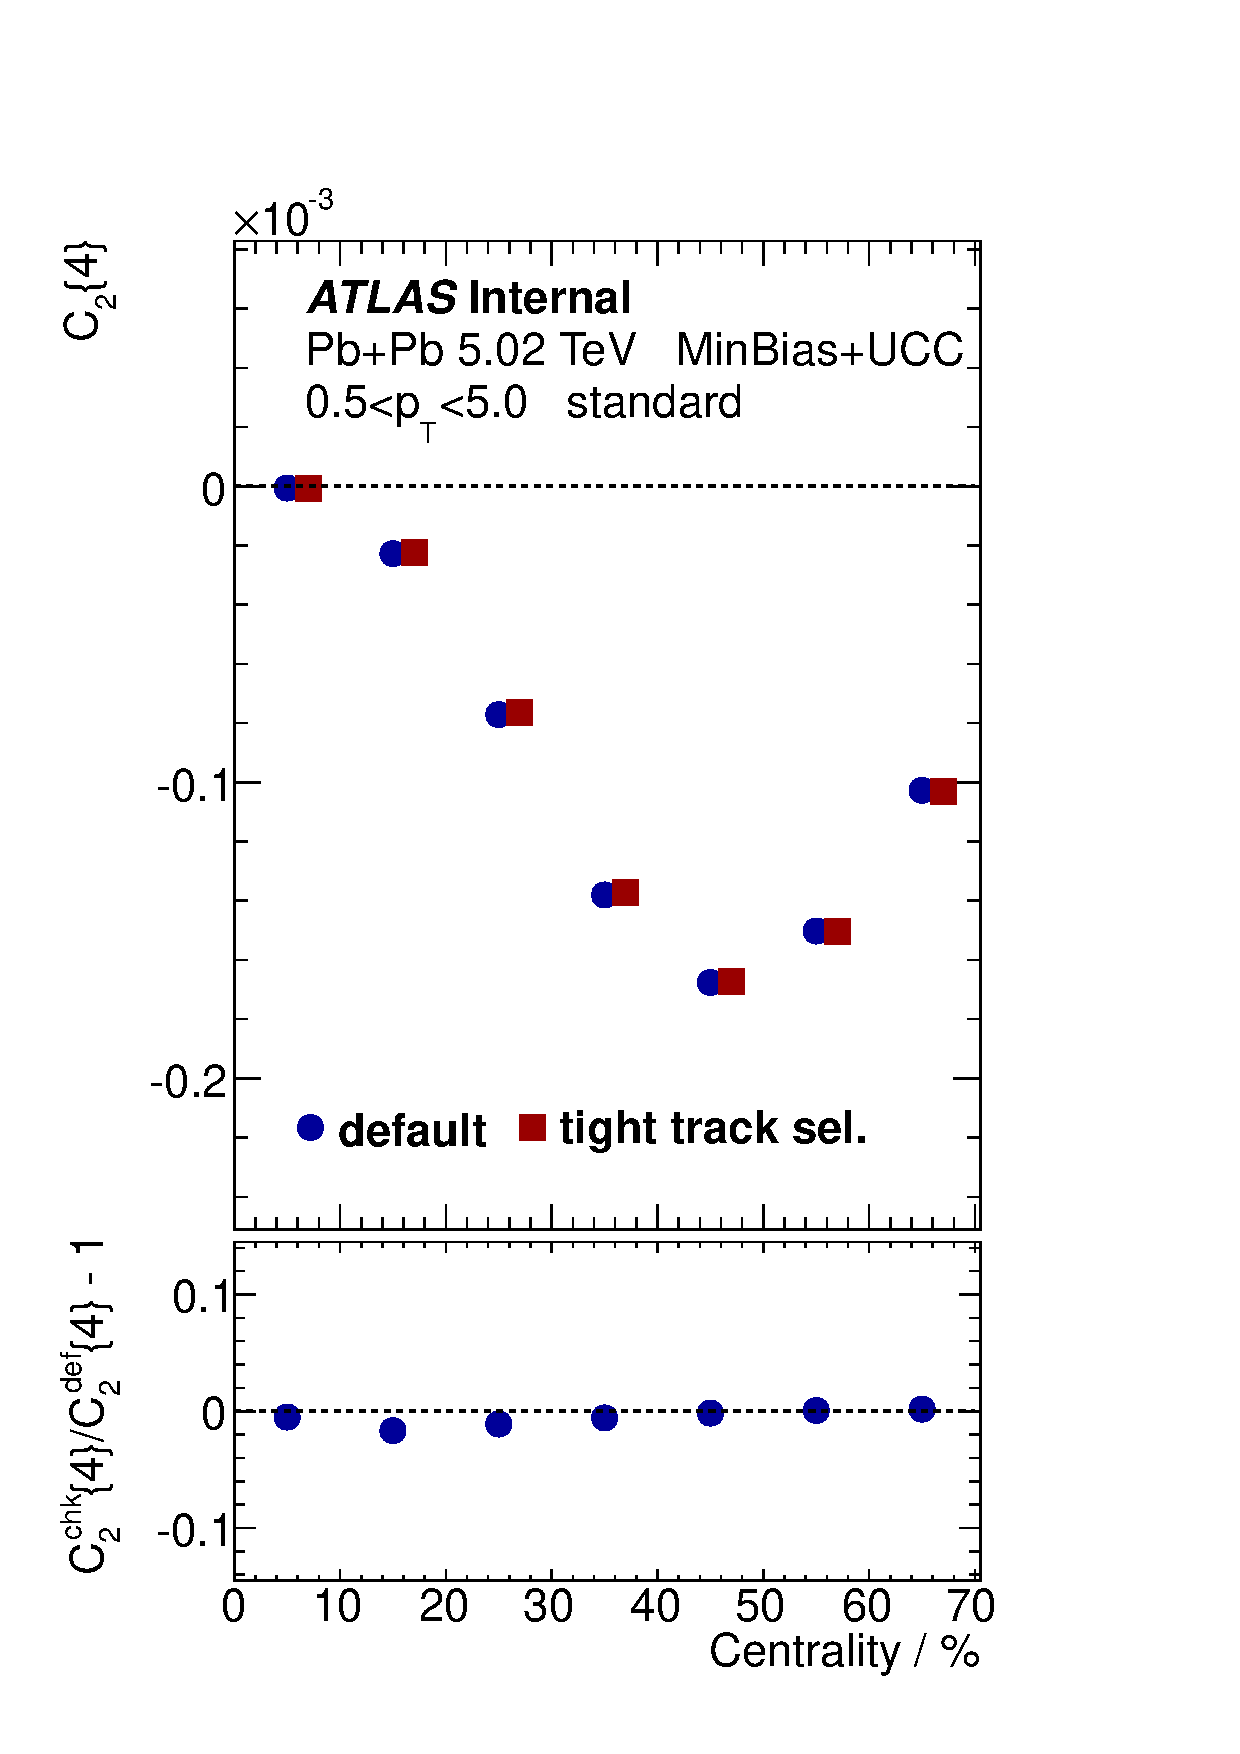
\includegraphics[width=.24\linewidth]{figs/chapter_appendix/trkSel_Har2.pdf}
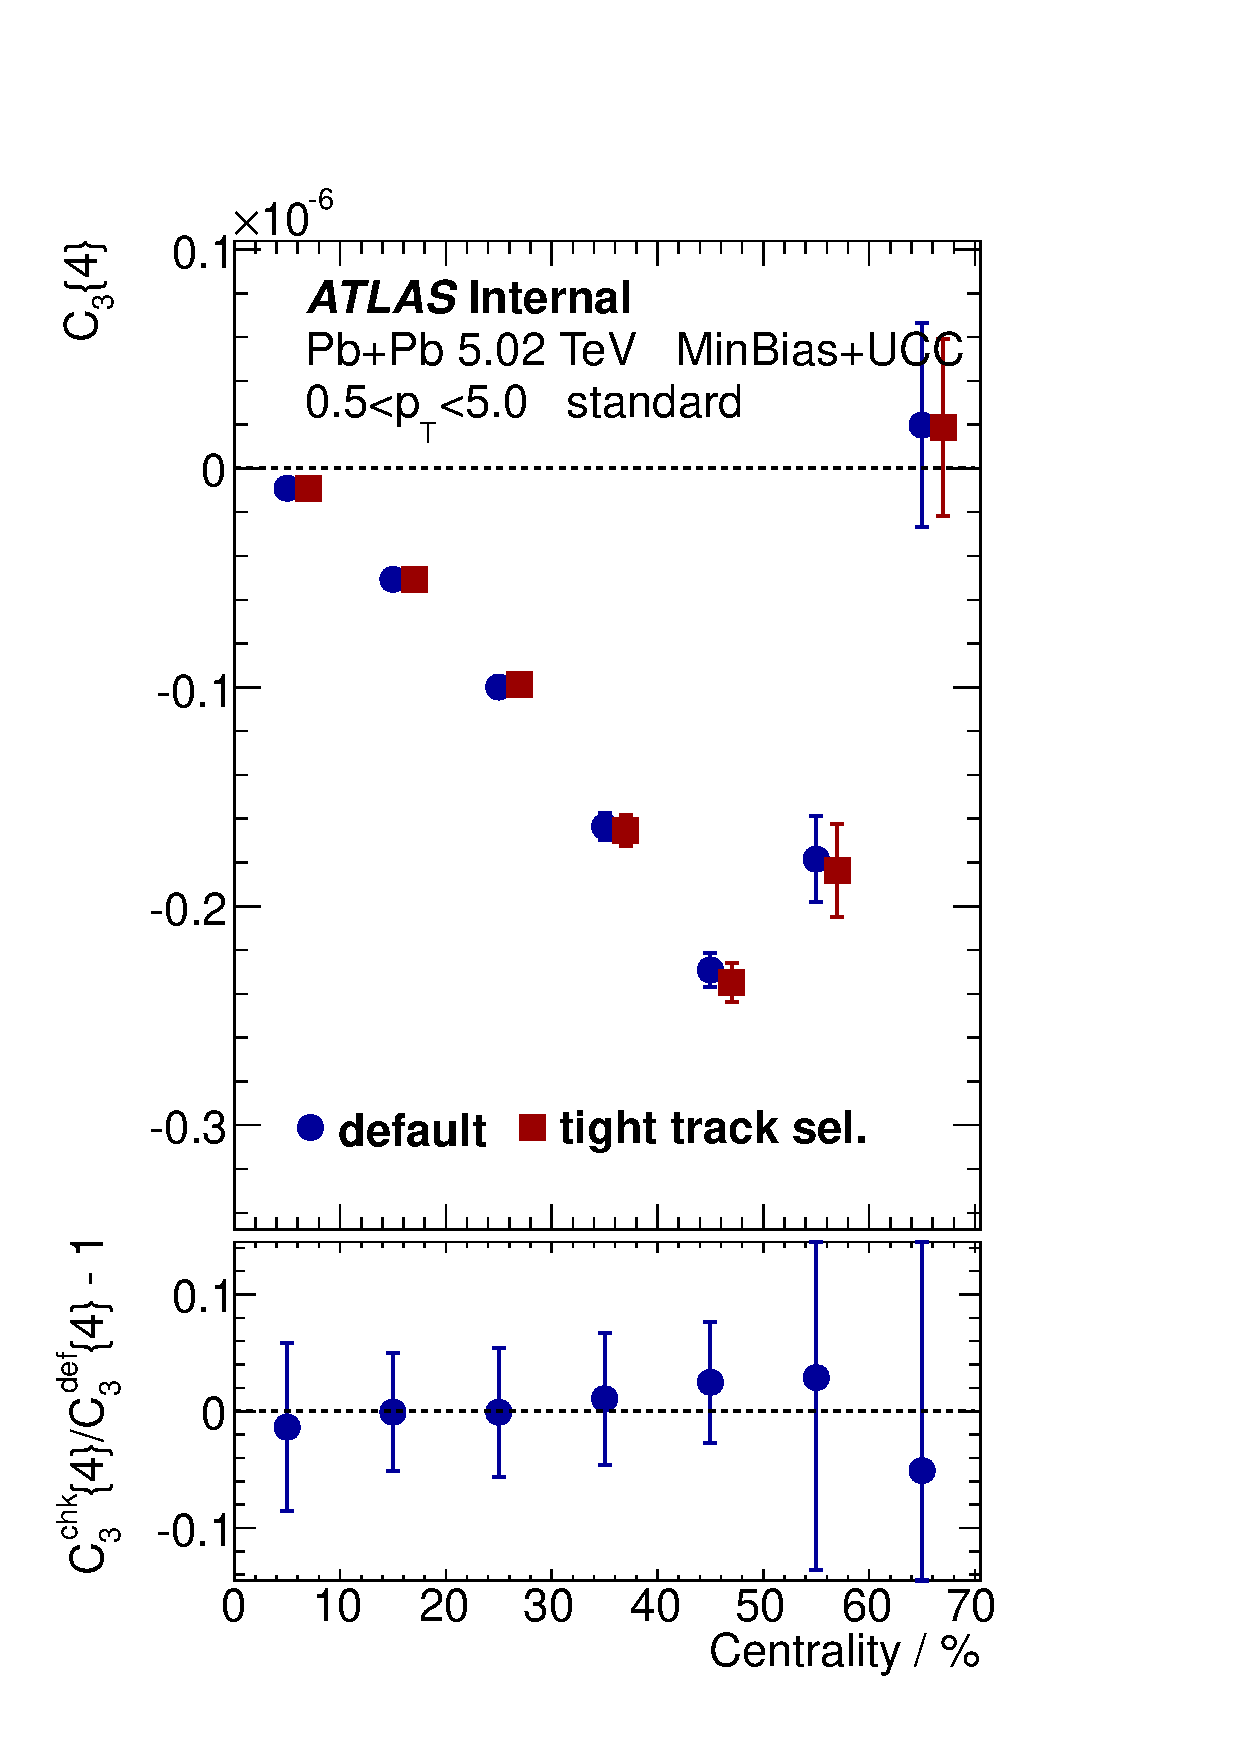
\includegraphics[width=.24\linewidth]{figs/chapter_appendix/trkSel_Har3.pdf}
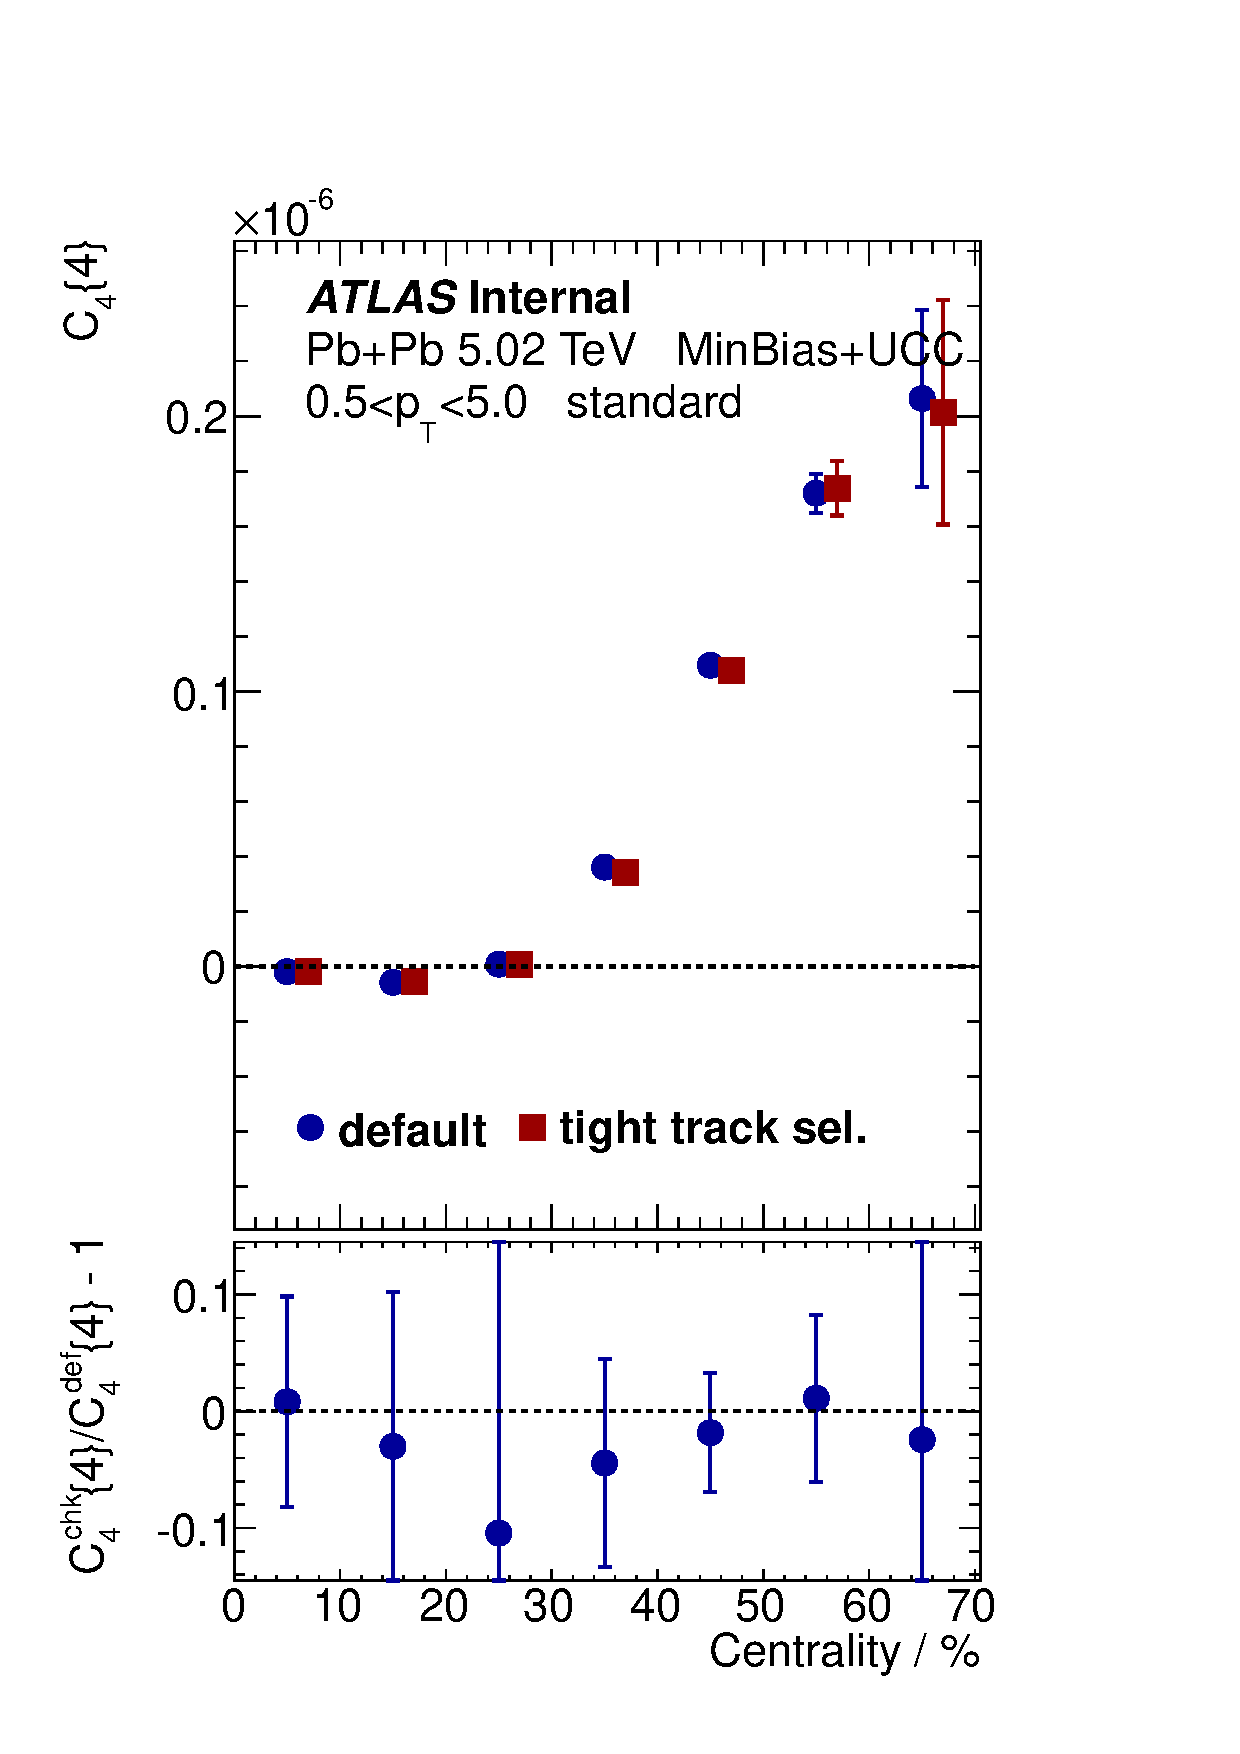
\includegraphics[width=.24\linewidth]{figs/chapter_appendix/trkSel_Har4.pdf}
\caption{Systematics of $c_n\{4\}$ from track selections: HI loose v.s. HI tight. Bottom panels are the relative uncertainties between the default and check.}
\label{fig:appendix_trkSel}
\end{figure}



\subsubsection{Tracking efficiency}
\label{sec:tracking_efficiency}

In this analysis, tracking efficiency is evaluated as a function of $\pT$, $\eta$ and centrality. Previous flow measurements have shown that $v_n$ strongly depends on $\pT$: it increases then decreases as $\pT$ increases. Meanwhile, differential flow measurements also shows that $v_n$ is weakly dependent of $\eta$. Due to these reasons, the $\pT$ weighting in tracking efficiency could introduce uncertainty to the results.

To evaluate the impact from uncertainty in the tracking efficiency, the following checks are performed:
\begin{itemize}
\item Default $\epsilon$: particles weighted by tracking efficiency;
\item Check 1 higher efficiency $\epsilon_+$: tracking efficiency in high $\pT$ is increased to its maximum within uncertainty; while tracking efficiency in low $\pT$ is decreased to its minimum within uncertainty;
\item Check 2 lower efficiency $\epsilon_-$: tracking efficiency in high $\pT$ is decreased to its minimum within uncertainty; while tracking efficiency in low $\pT$ is increased to its maximum within uncertainty;
\end{itemize}
where the two checks can be parameterized as:
\begin{equation}
\epsilon_\pm(\pT) \equiv \epsilon(\pT) \pm 0.06\frac{\epsilon(\pT)-\epsilon(\pT^\text{low})}{\epsilon(\pT^\text{high})-\epsilon(\pT^\text{low})} \mp 0.03
\end{equation}
where $\pT^\text{low}$ is 0.5 GeV while $\pT^\text{high}$ is 5.0 GeV, which are the minimum and maximum $\pT$ ranges of this analysis.

Note that $0.03$ was selected as the variation of the tracking efficiency, which has been evaluated in the Minimum Bias multiplicity in 13 TeV $pp$ analysis~\cite{Morley:2011604}. The total uncertainty in tracking is shown in Fig.~\ref{fig:appendix_trkEff_err}, and the maximum variation for $p_\text{T}>0.5$ GeV is about $3\%$.
\begin{figure}[H]
\centering
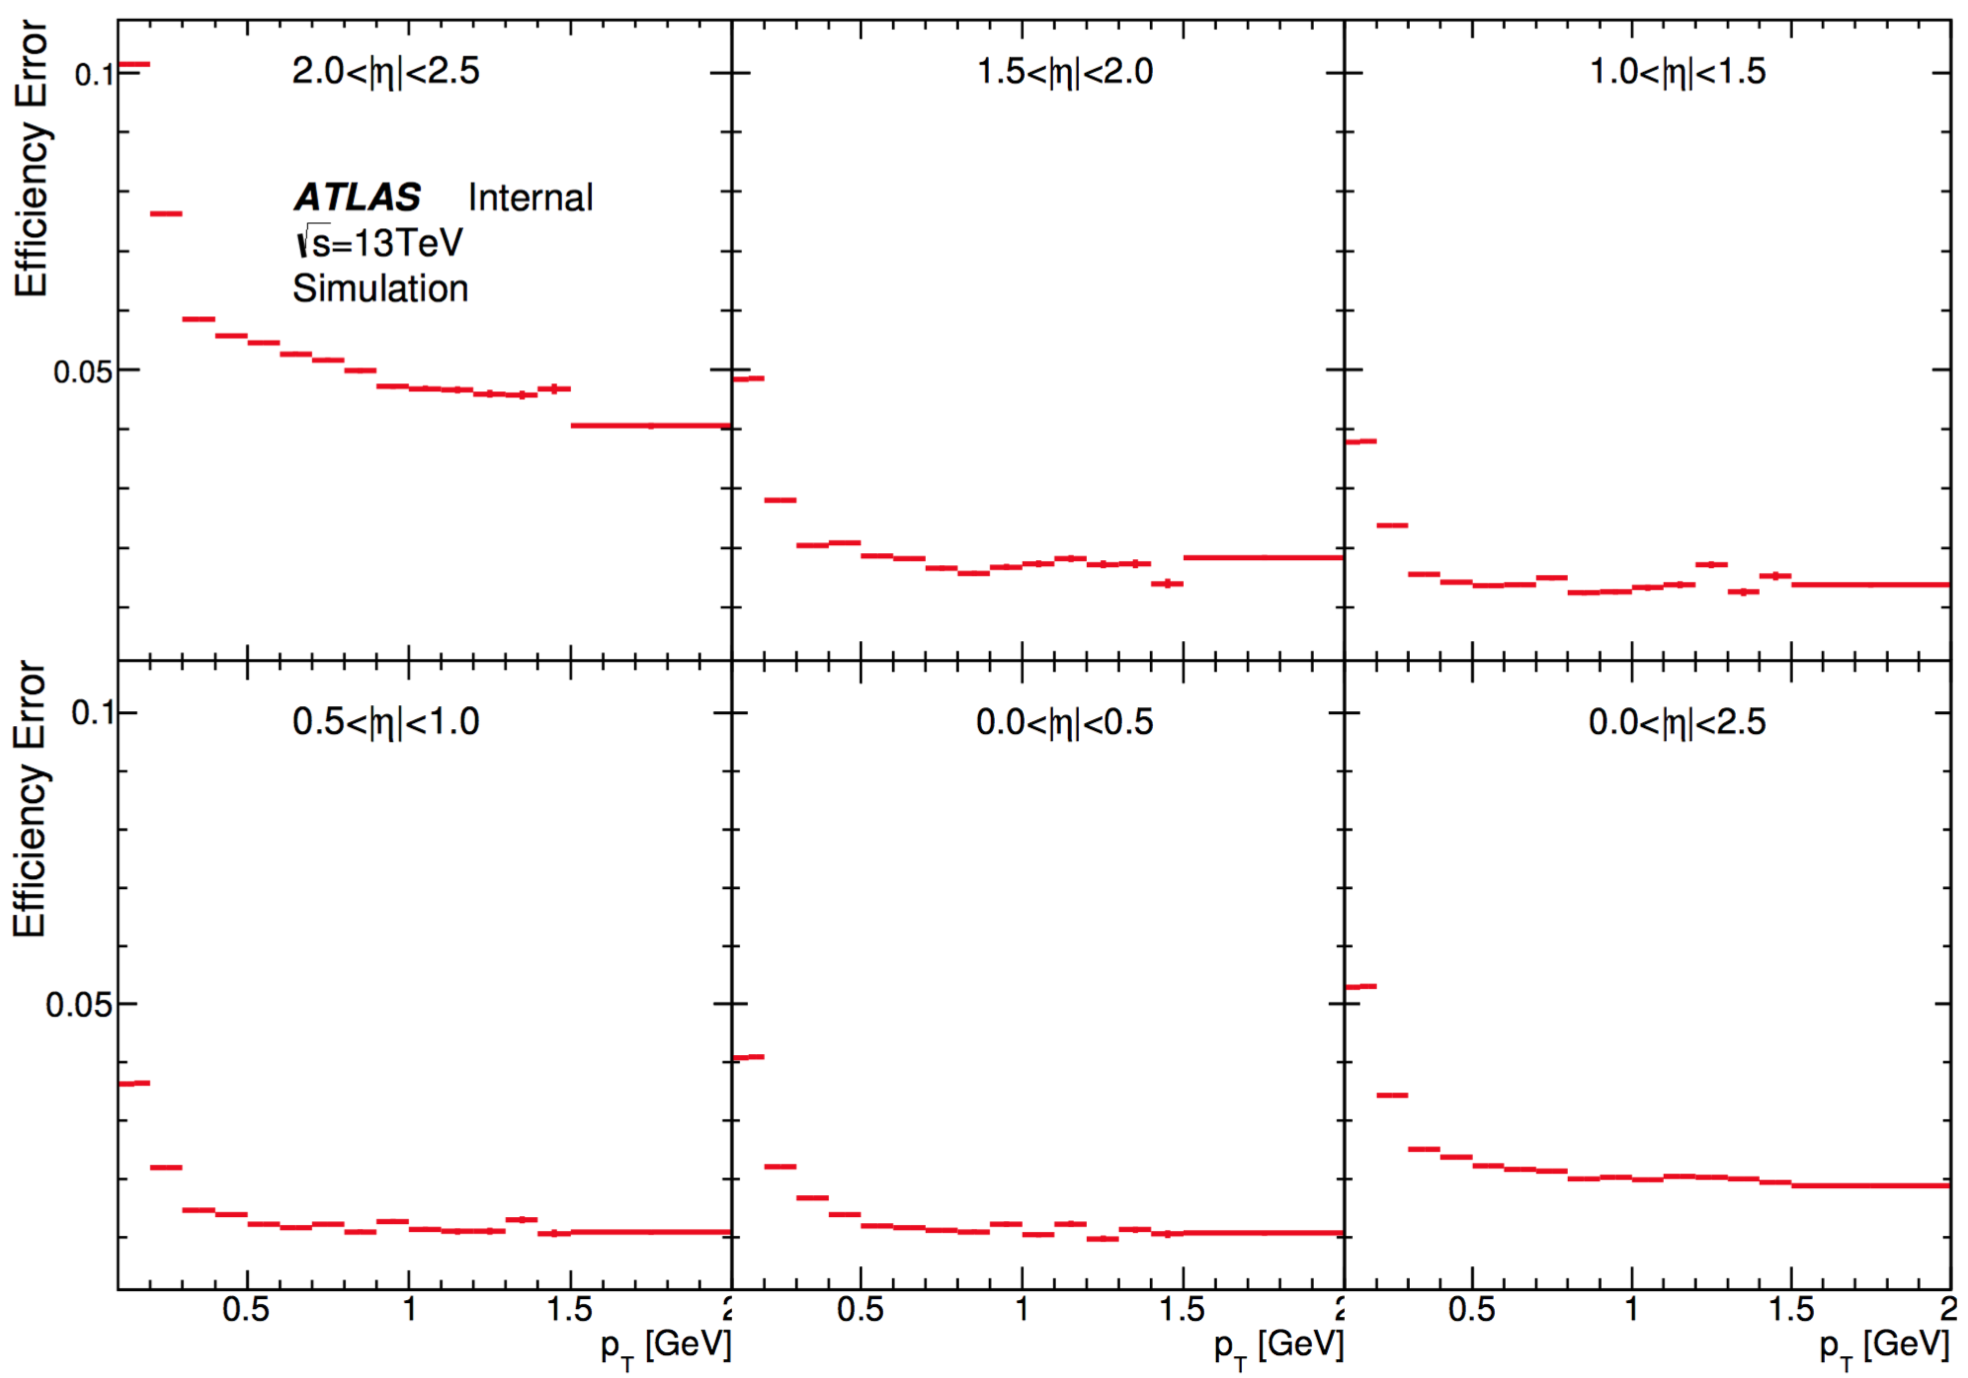
\includegraphics[width=.9\linewidth]{figs/chapter_appendix/trkEff_err.png}
\caption{The systematic uncertainties of the tracking efficiency plotted as a function of $\pT$ for several $|\eta|$ slices. These include the material uncertainties.}
\label{fig:appendix_trkEff_err}
\end{figure}

Fig.~\ref{fig:appendix_trkEff1} and fig.~\ref{fig:appendix_trkEff2} show the comparison of $c_n\{4\}$ calculated using default tracking efficiency and lower/higher variations. For all the harmonics, the relative differences have opposite sign between lower and higher efficiency, as expected due to the $\pT$ dependence of flow. The largest relative differences come from low $\pT$ range, and decrease quickly as minimum $\pT$ cut increase. This check will be quoted as part of the combined systematics.
\begin{figure}[H]
\centering
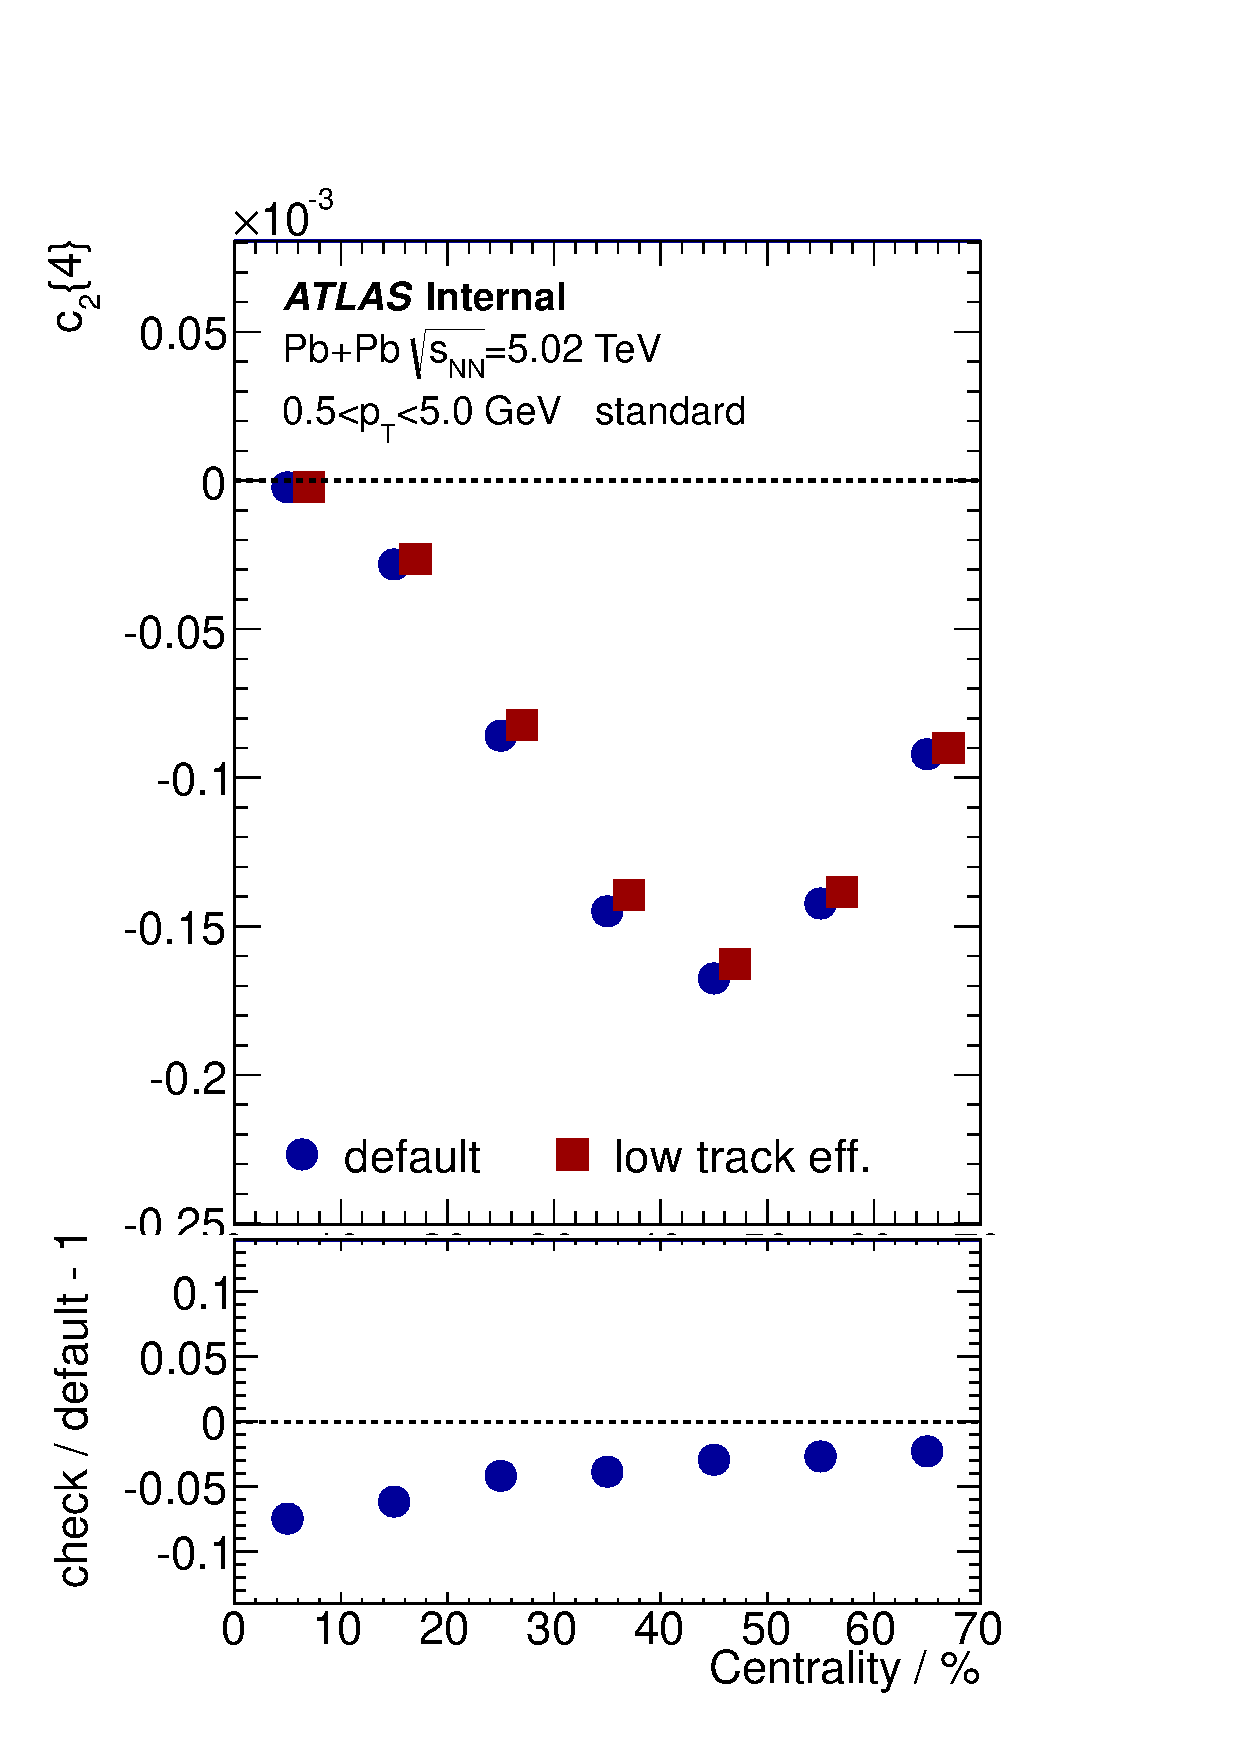
\includegraphics[width=.24\linewidth]{figs/chapter_appendix/trkEff1_Har2_Pt0.pdf}
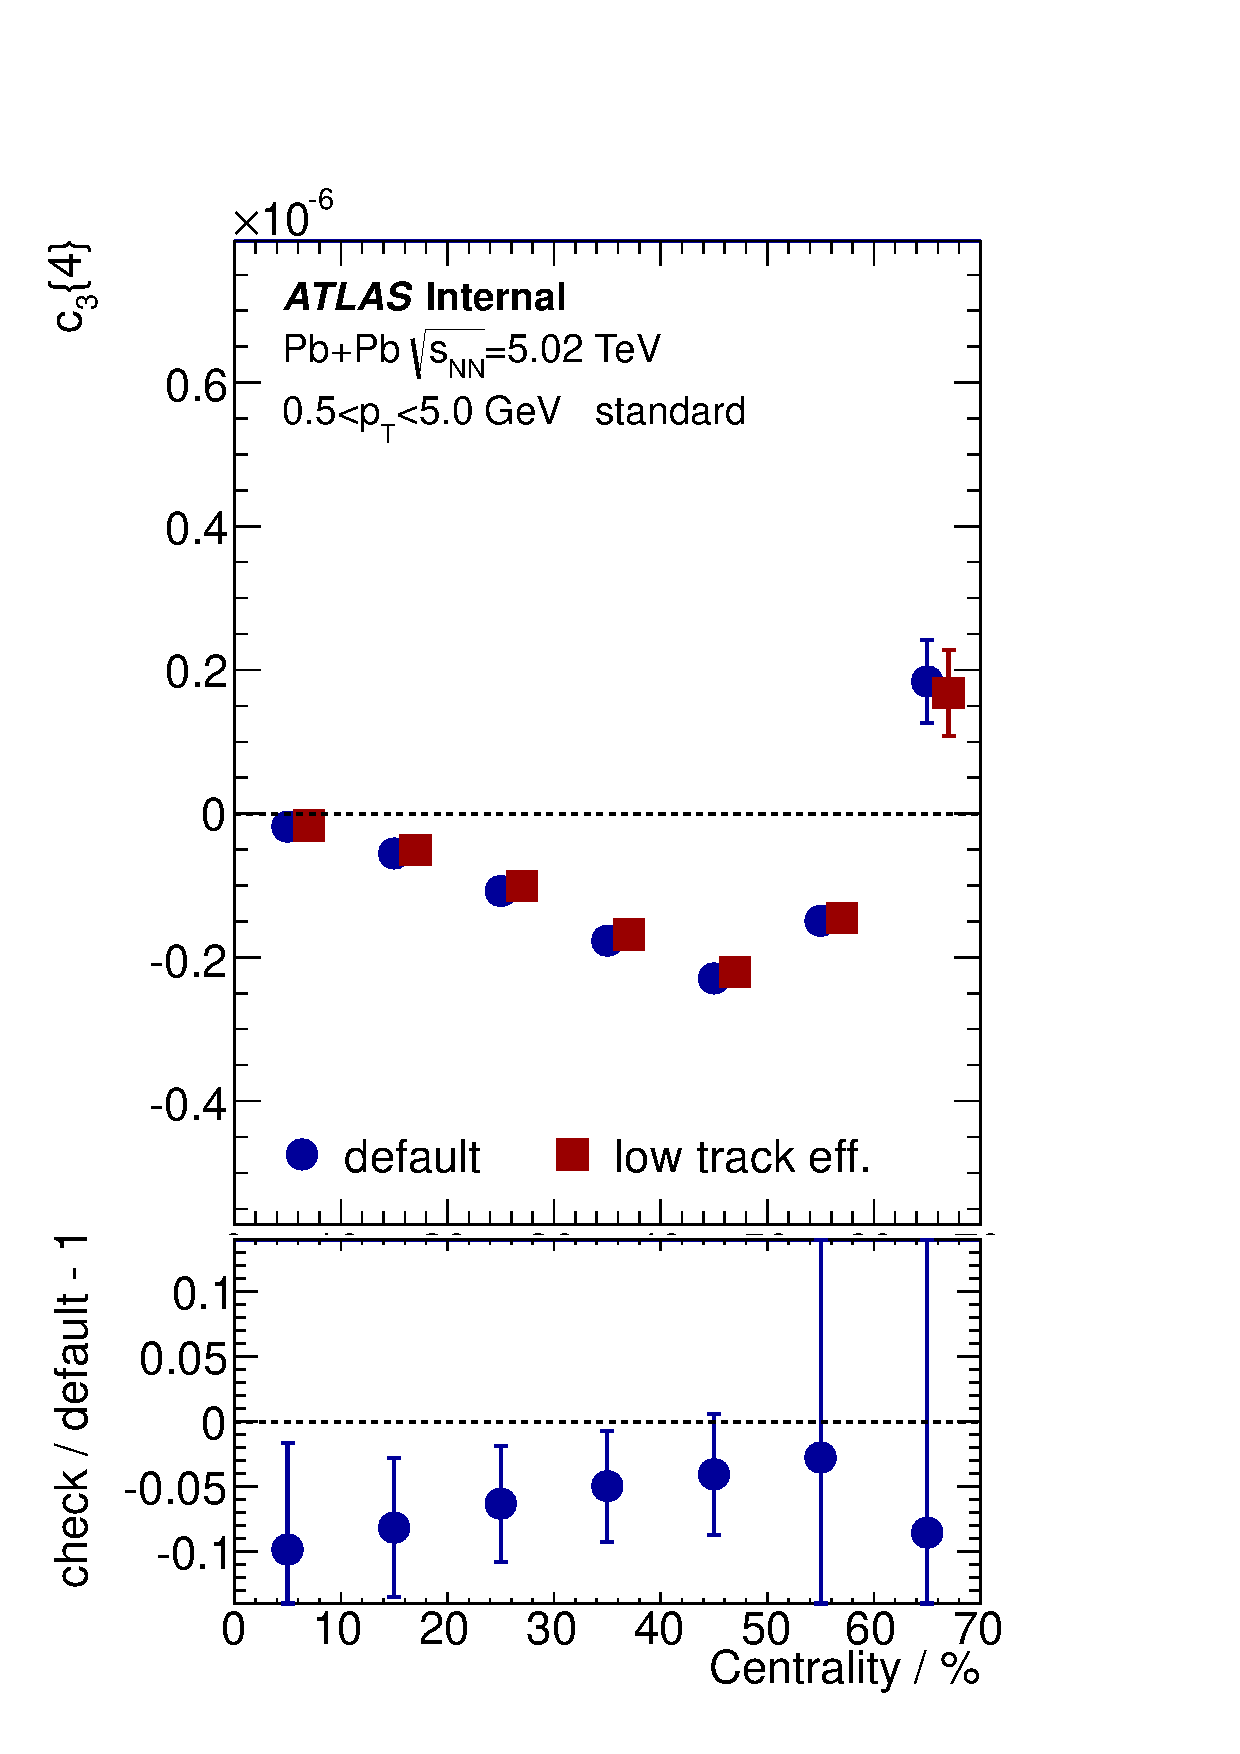
\includegraphics[width=.24\linewidth]{figs/chapter_appendix/trkEff1_Har3_Pt0.pdf}
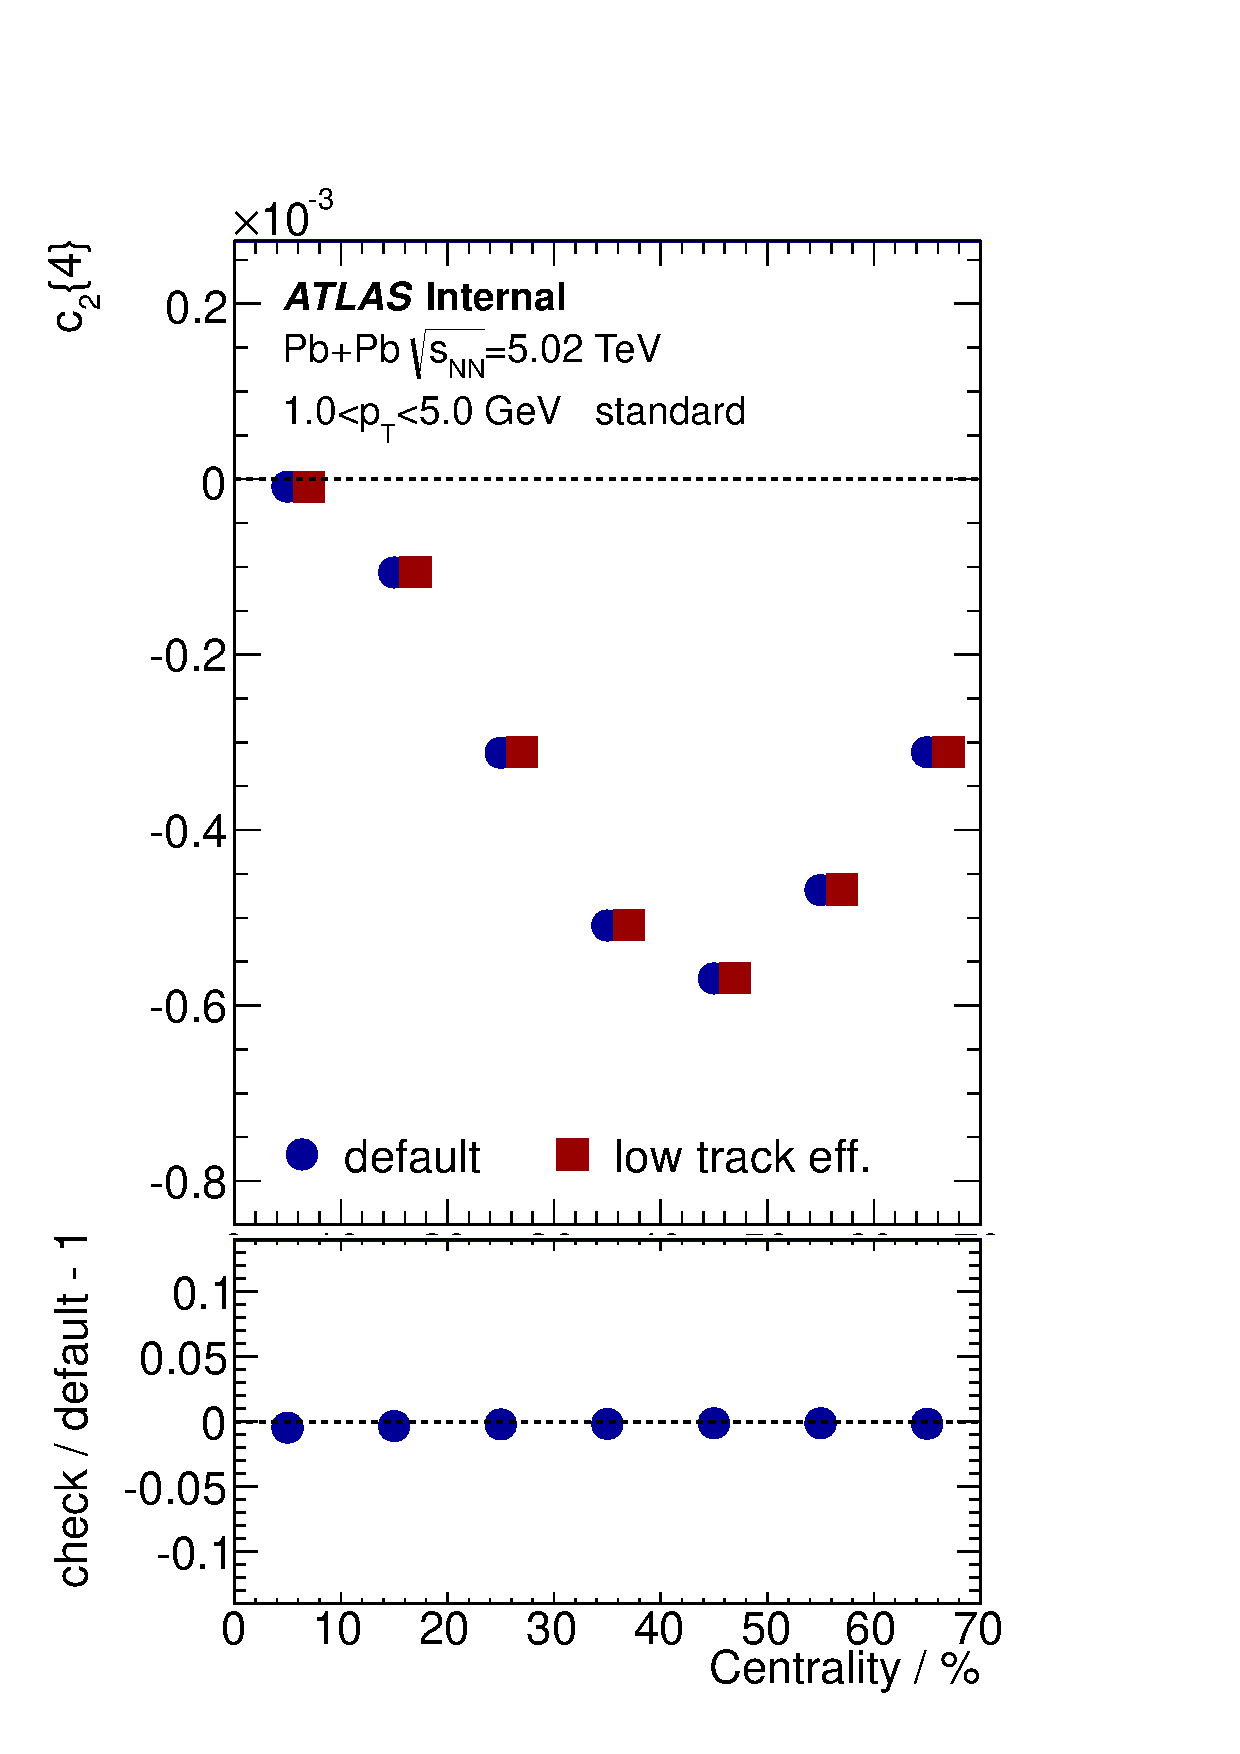
\includegraphics[width=.24\linewidth]{figs/chapter_appendix/trkEff1_Har2_Pt1.pdf}
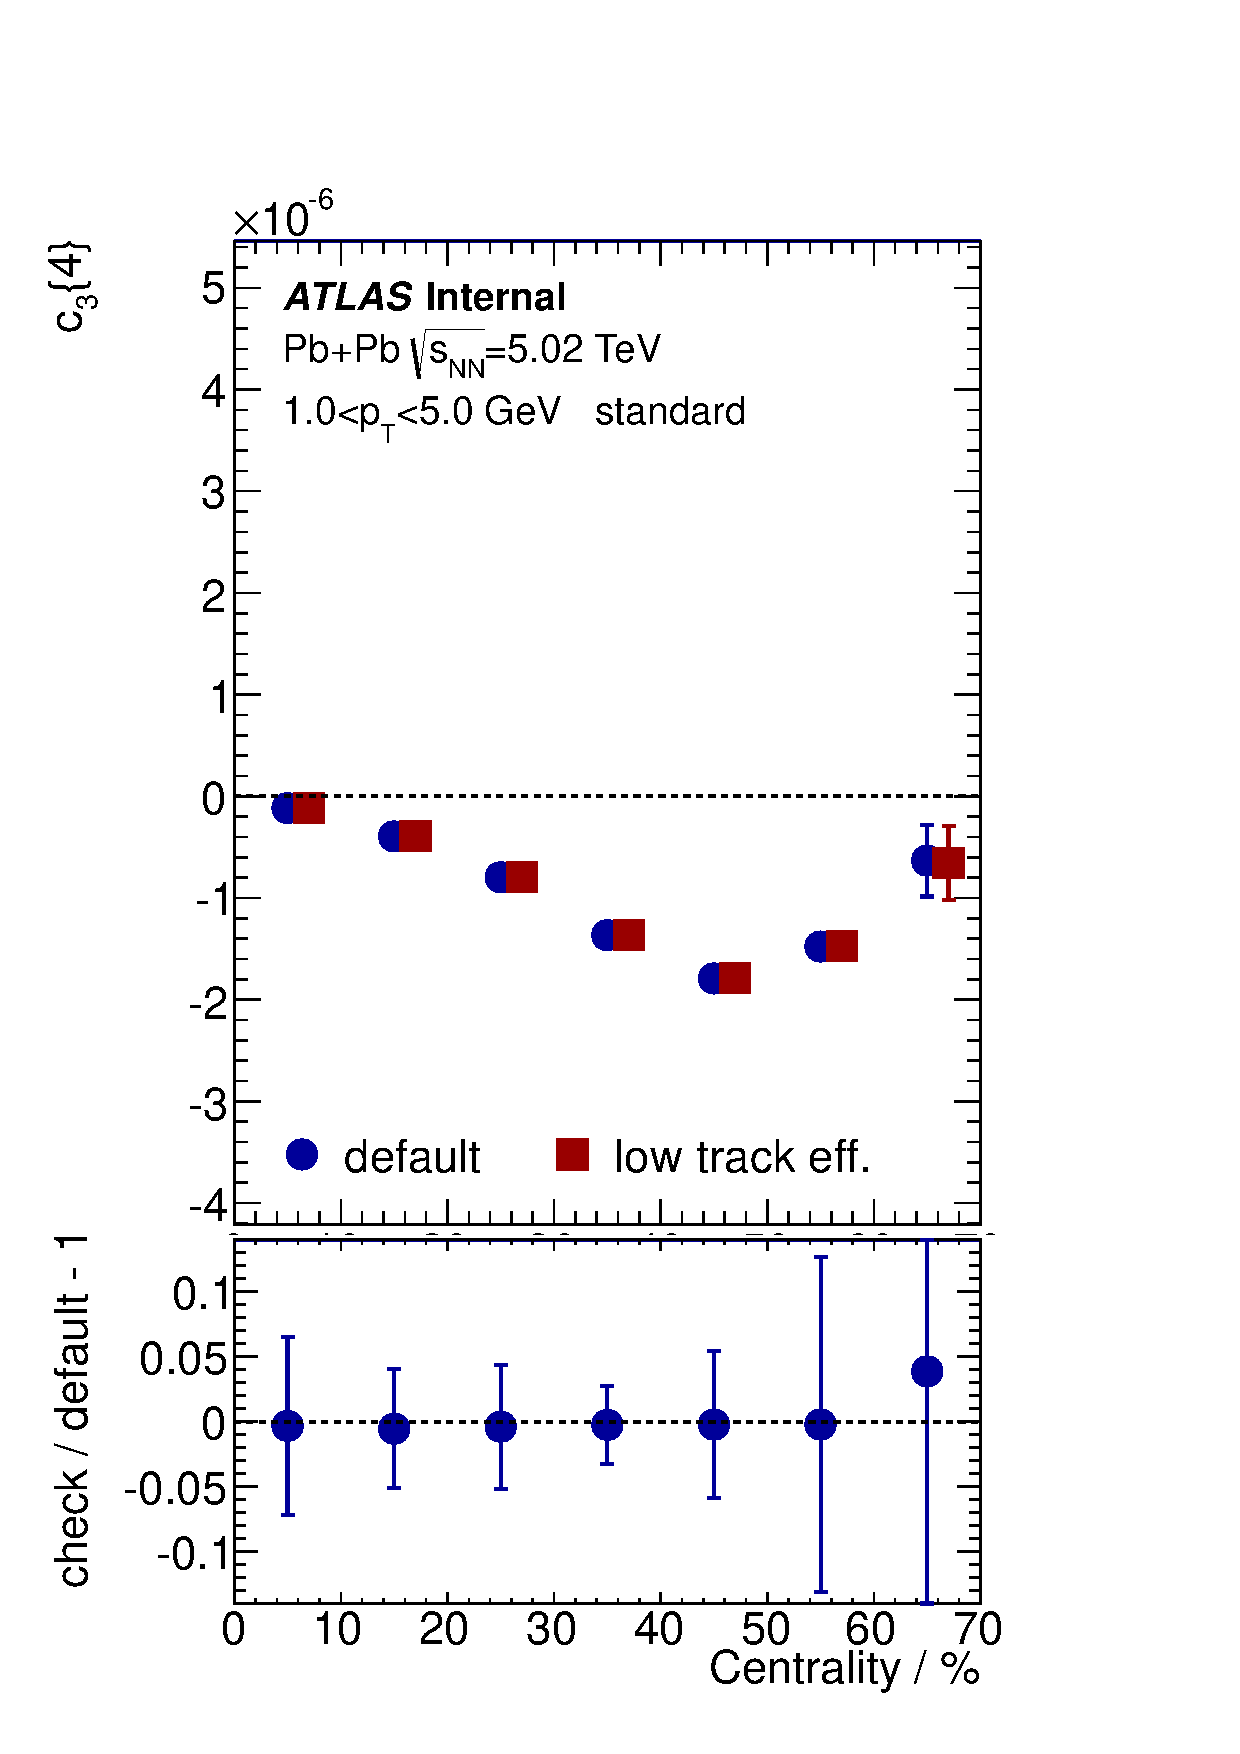
\includegraphics[width=.24\linewidth]{figs/chapter_appendix/trkEff1_Har3_Pt1.pdf}
\caption{Systematics of $c_n\{4\}$ from tracking efficiency: default v.s. lower efficiency. Bottom panels are the relative uncertainties between the default and check.}
\label{fig:appendix_trkEff1}
\end{figure}

\begin{figure}[H]
\centering
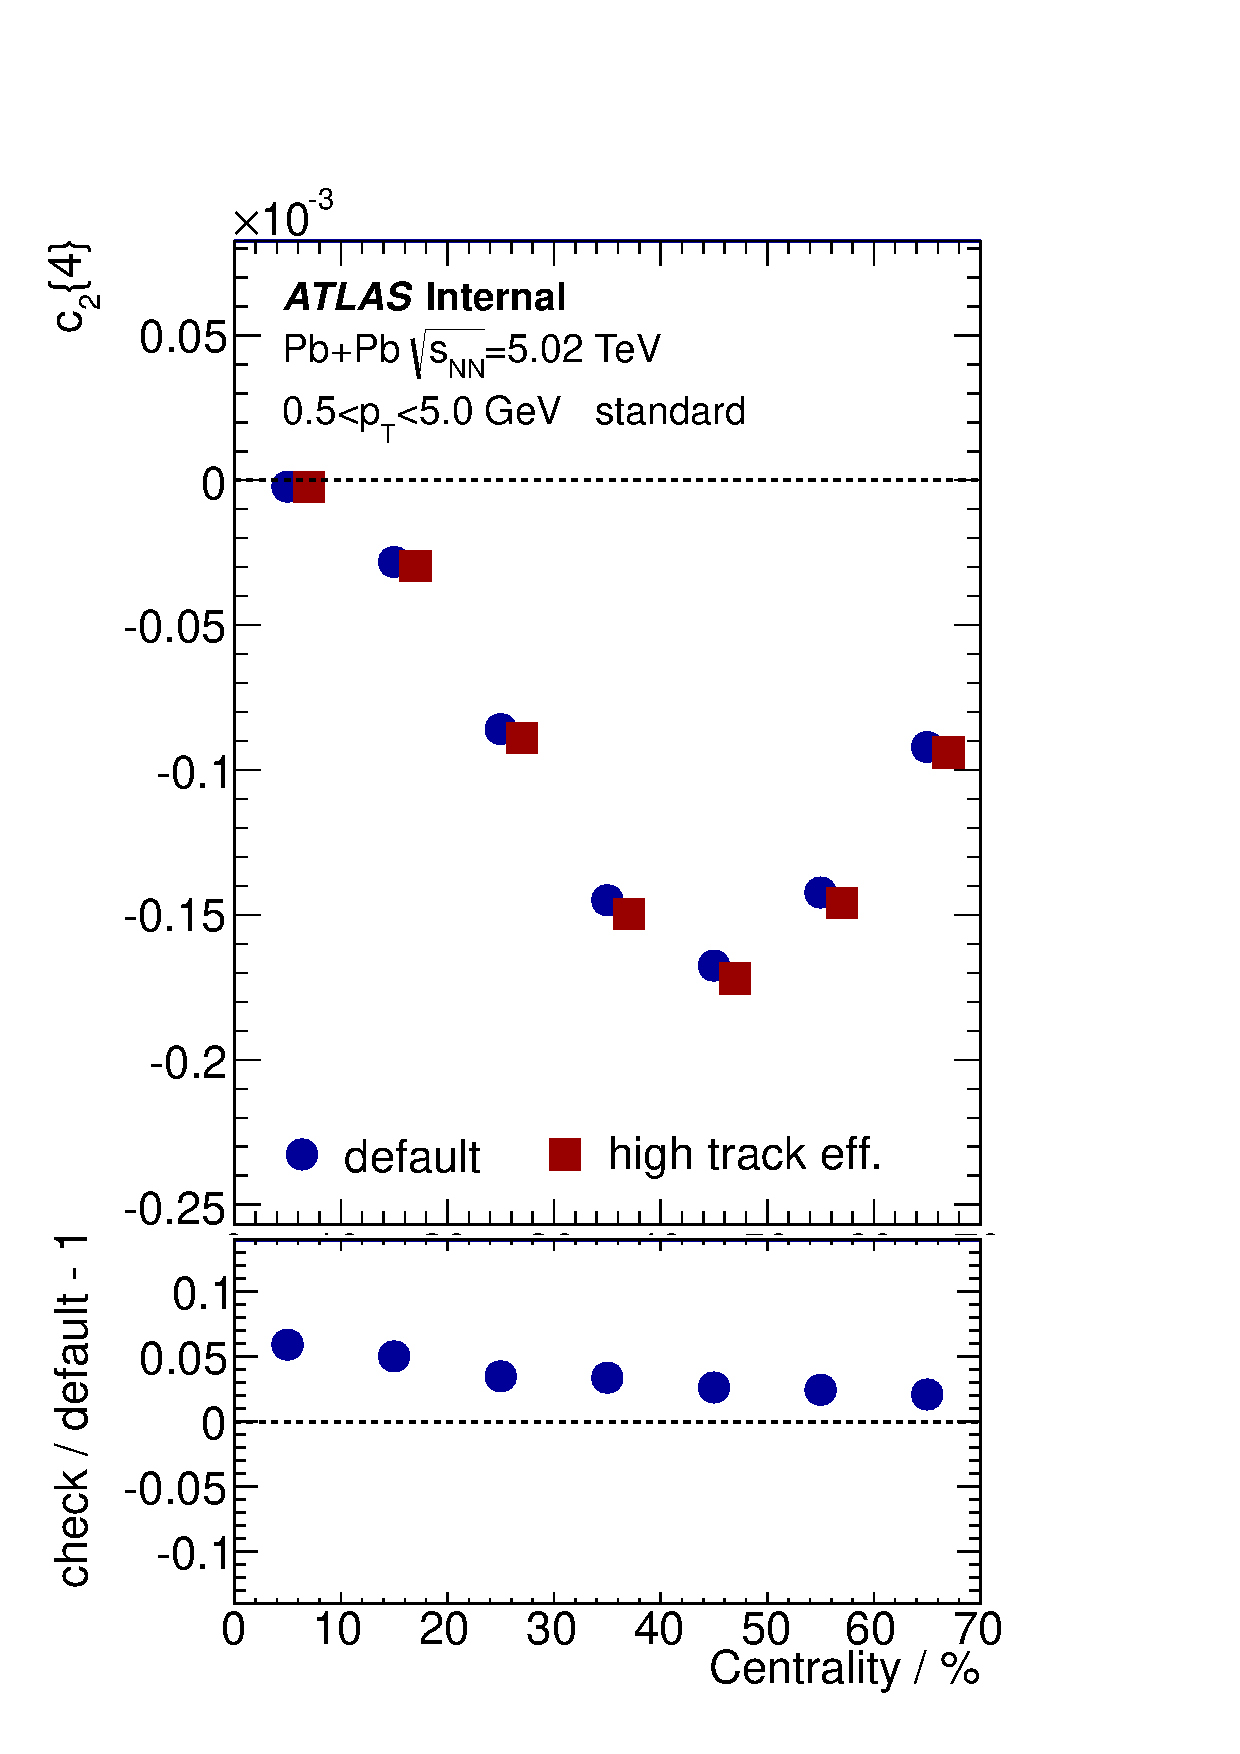
\includegraphics[width=.24\linewidth]{figs/chapter_appendix/trkEff2_Har2_Pt0.pdf}
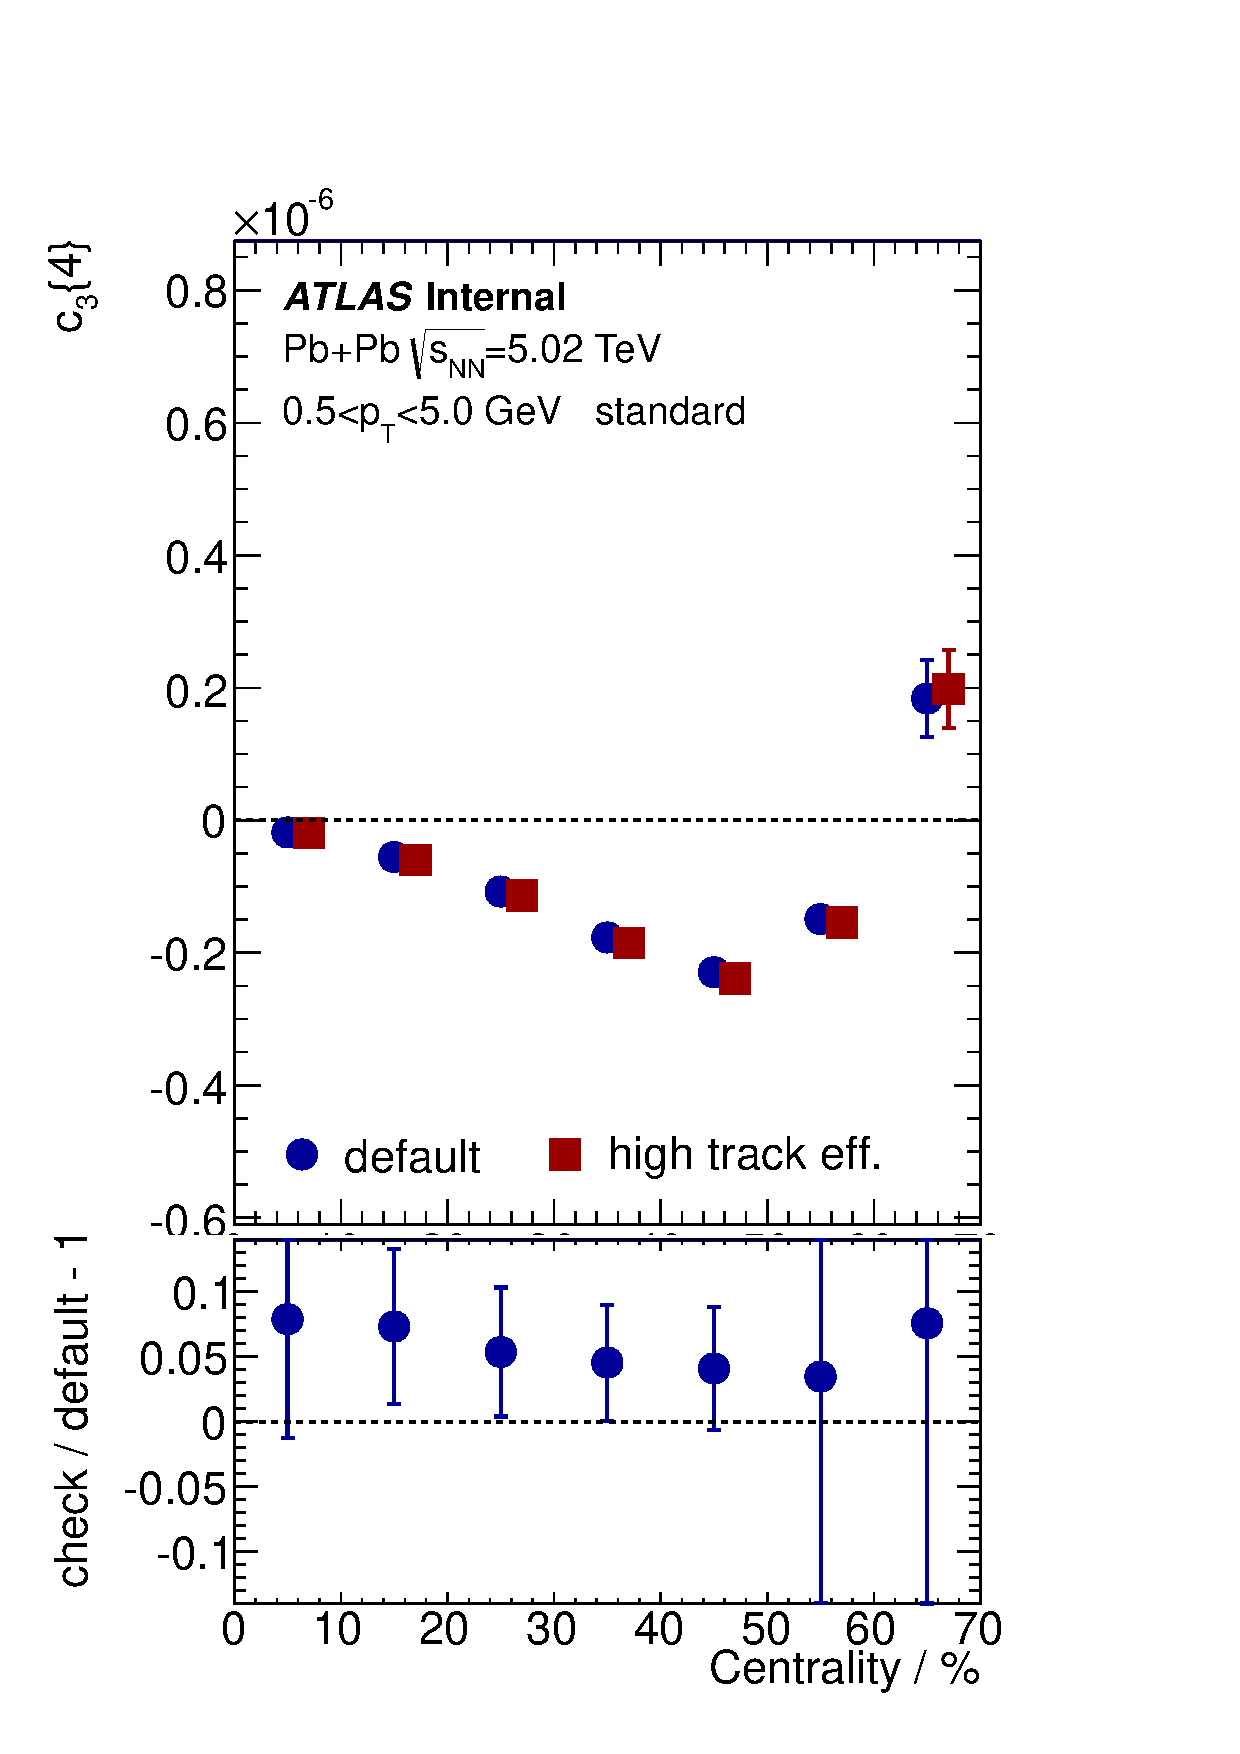
\includegraphics[width=.24\linewidth]{figs/chapter_appendix/trkEff2_Har3_Pt0.pdf}
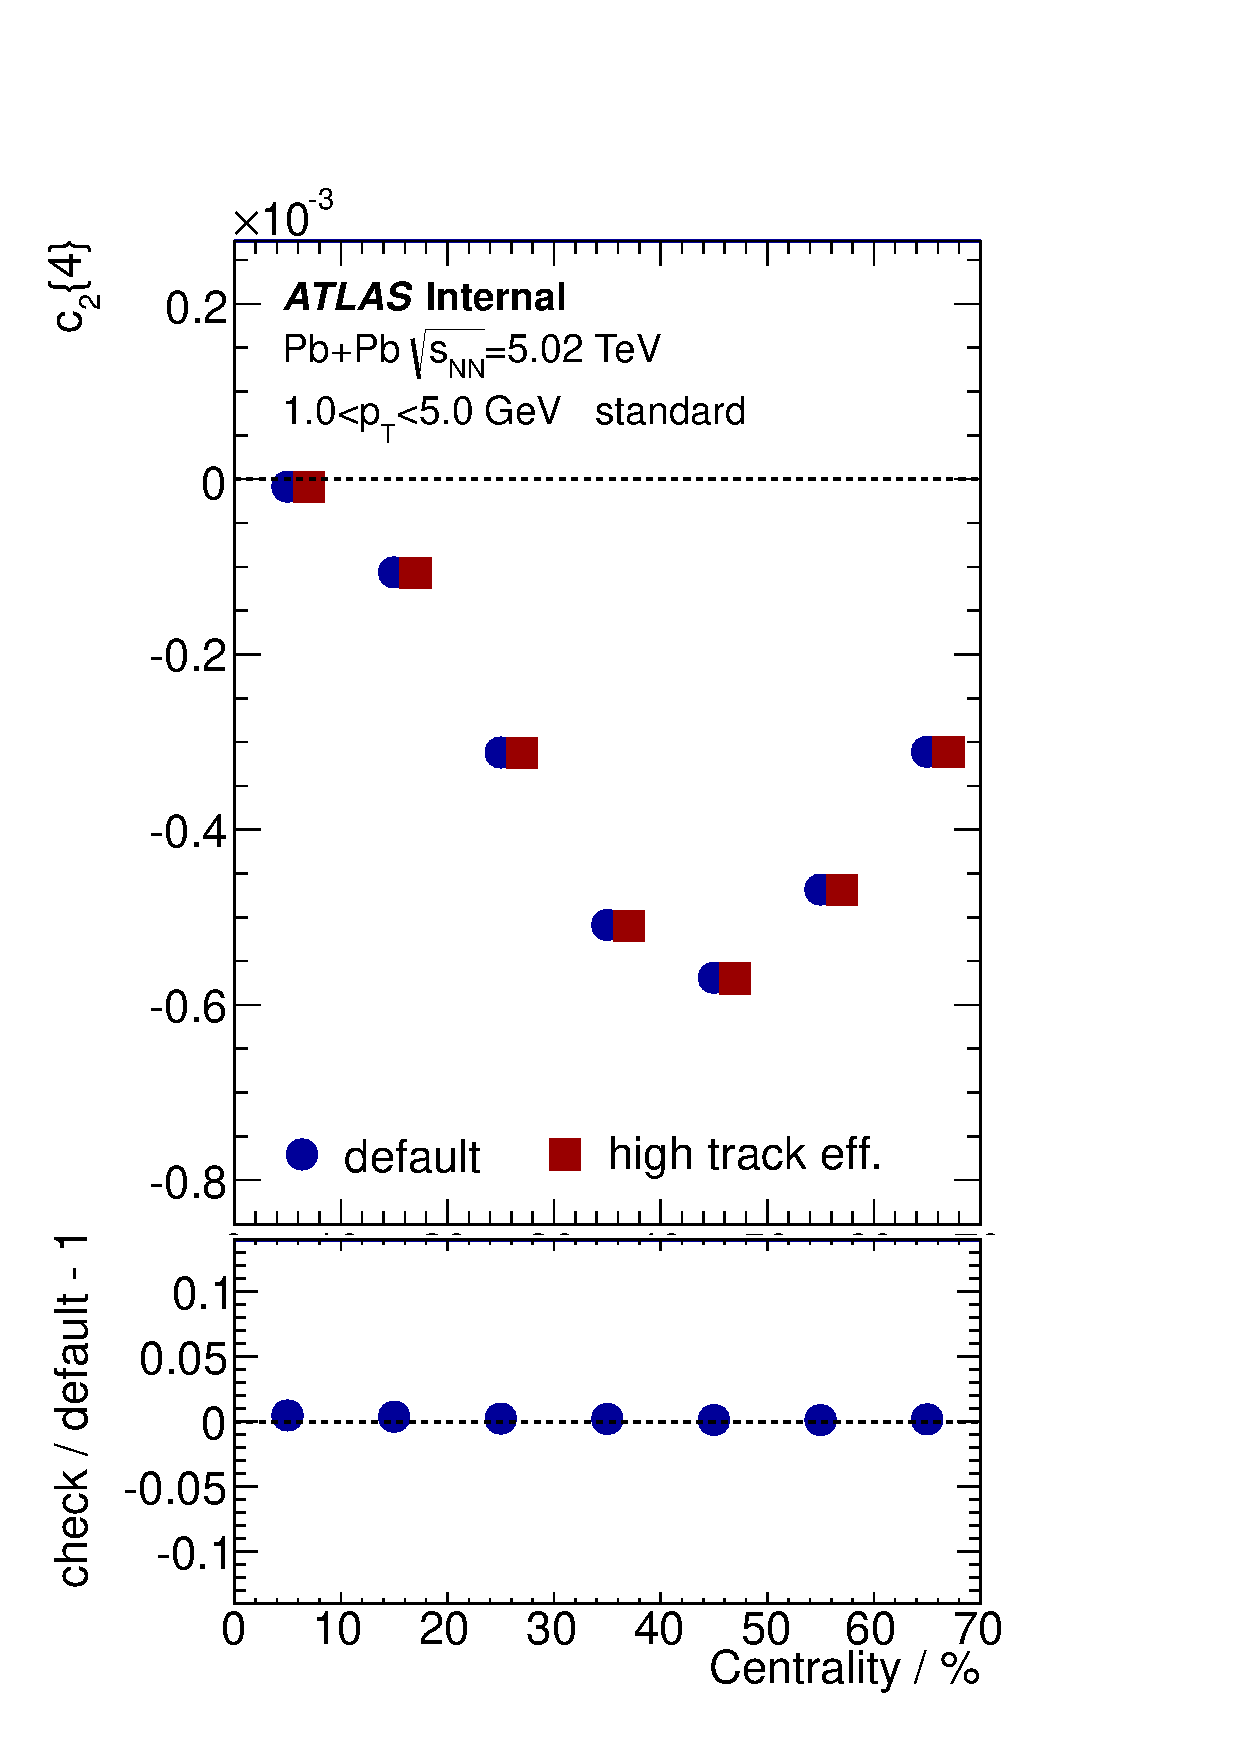
\includegraphics[width=.24\linewidth]{figs/chapter_appendix/trkEff2_Har2_Pt1.pdf}
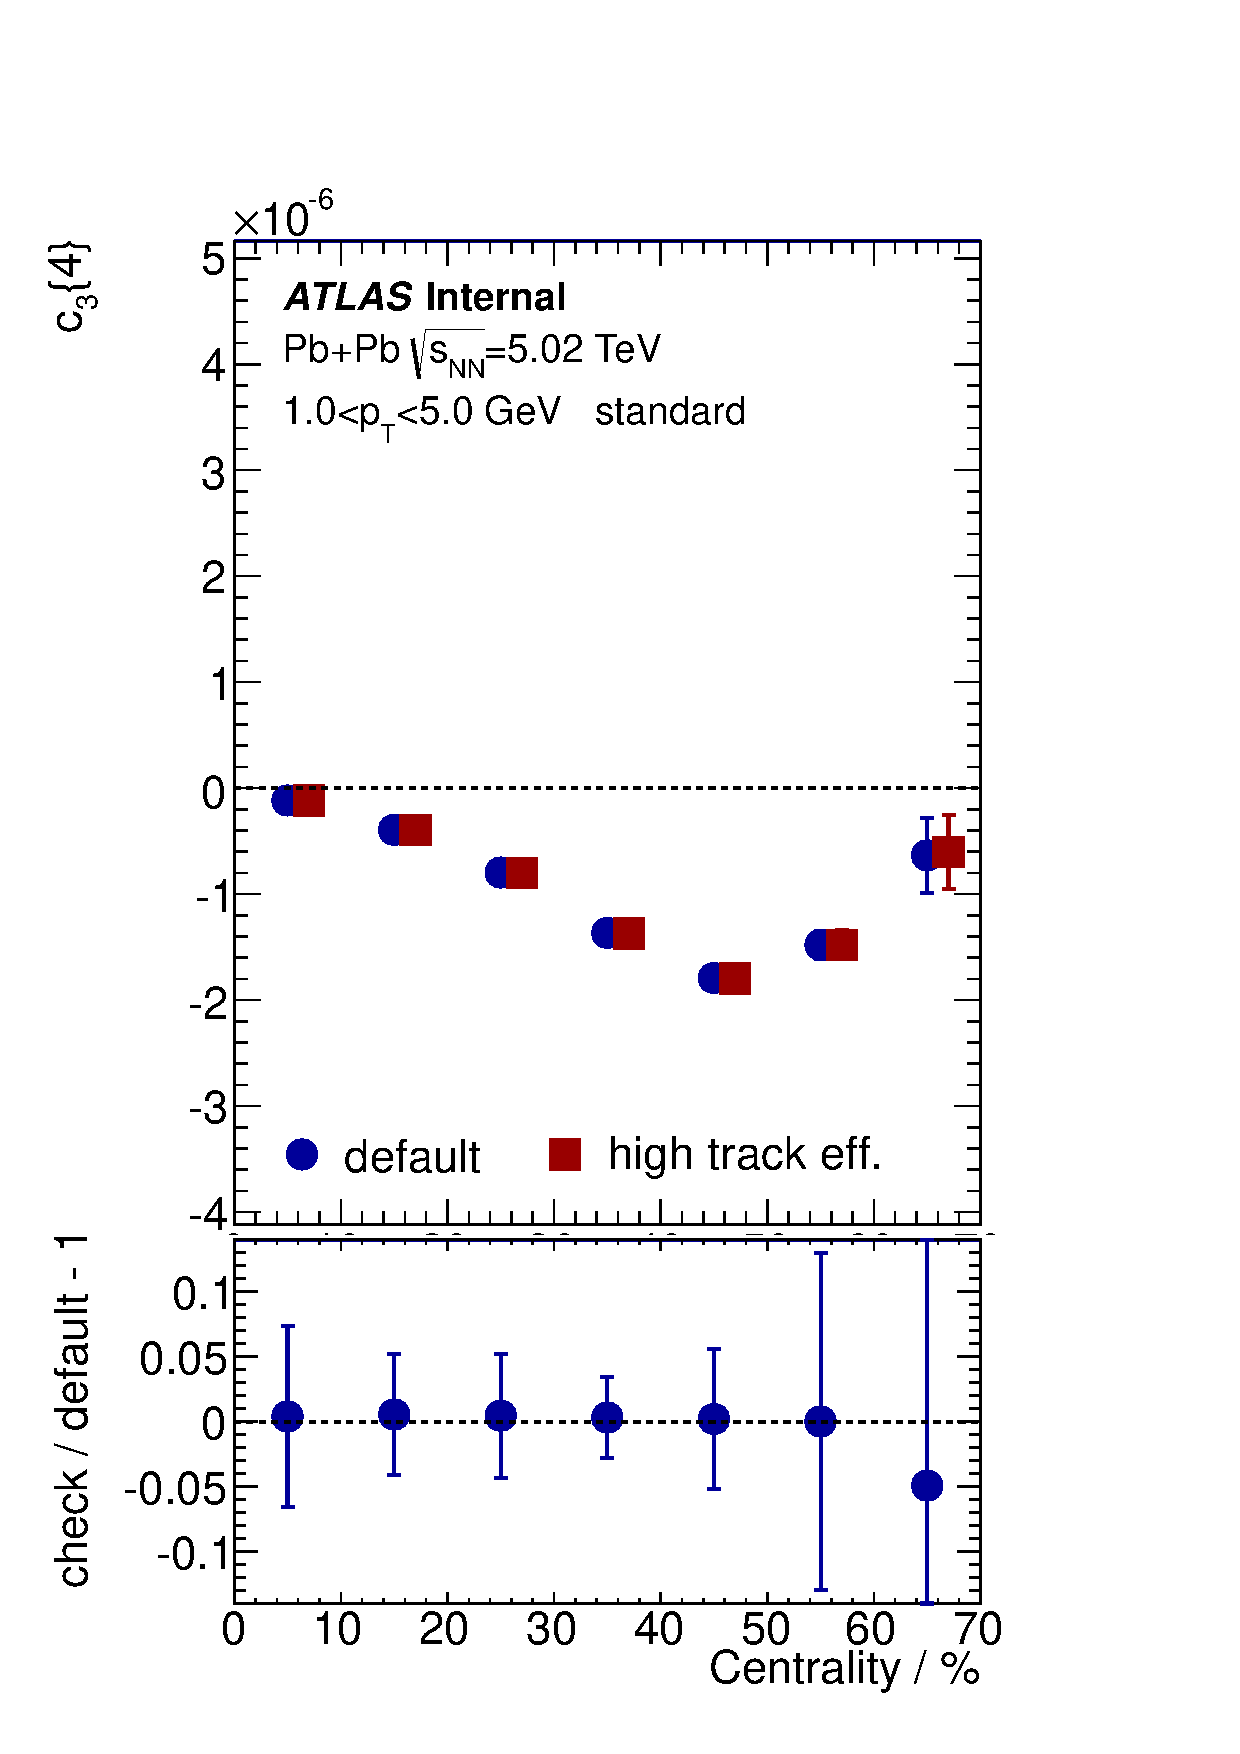
\includegraphics[width=.24\linewidth]{figs/chapter_appendix/trkEff2_Har3_Pt1.pdf}
\caption{Systematics of $c_n\{4\}$ from tracking efficiency: default v.s. higher efficiency. Bottom panels are the relative uncertainties between the default and check.}
\label{fig:appendix_trkEff2}
\end{figure}



\subsubsection{Summary}

This section summarizes the breakdown of systematics for every observable in this analysis. In order not to flooding the plots, the results are shown in two $\pT$ ranges:
\begin{itemize}
\item $0.5<\pT<5.0$ GeV;
\item $1.0<\pT<5.0$ GeV;
\end{itemize}
and except for the 2-particle cumulant, all other results are only shown using standard cumulant method. The corresponding systematics from 3-subevent method is listed in the Appendix.

Overall, the summary of systematics has the following features:
\begin{itemize}
\item In most cases, systematics are dominated by tracking efficiency variations. This is not surprising since magnitude of flow, as well as its fluctuation, are highly dependent of $\pT$. Slightly change in tracking efficiency as a function of $\pT$ will cause noticeable differences to cumulants;
\item Monte-Carlo closure has significant impact on $c_n\{2k\}$: in the lower $\pT$ region, about $5\%$ for 2-particle cumulant, $10\%$ and $15\%$ for 4- and 6-particle cumulants. In higher $\pT$, systematics from MC closure become much smaller;
\item Normalized cumulant, symmetric cumulant and asymmetric cumulant have smaller systematic errors than its correspondence without normalization, due to the reason that part of the systematics are canceled out in the ratio;
\end{itemize}

As a summary, in most cases, the total systematics are within $10\%$. In other cases where the systematics are larger, they are still smaller or comparable with statistical uncertainties.

\begin{figure}[H]
\centering
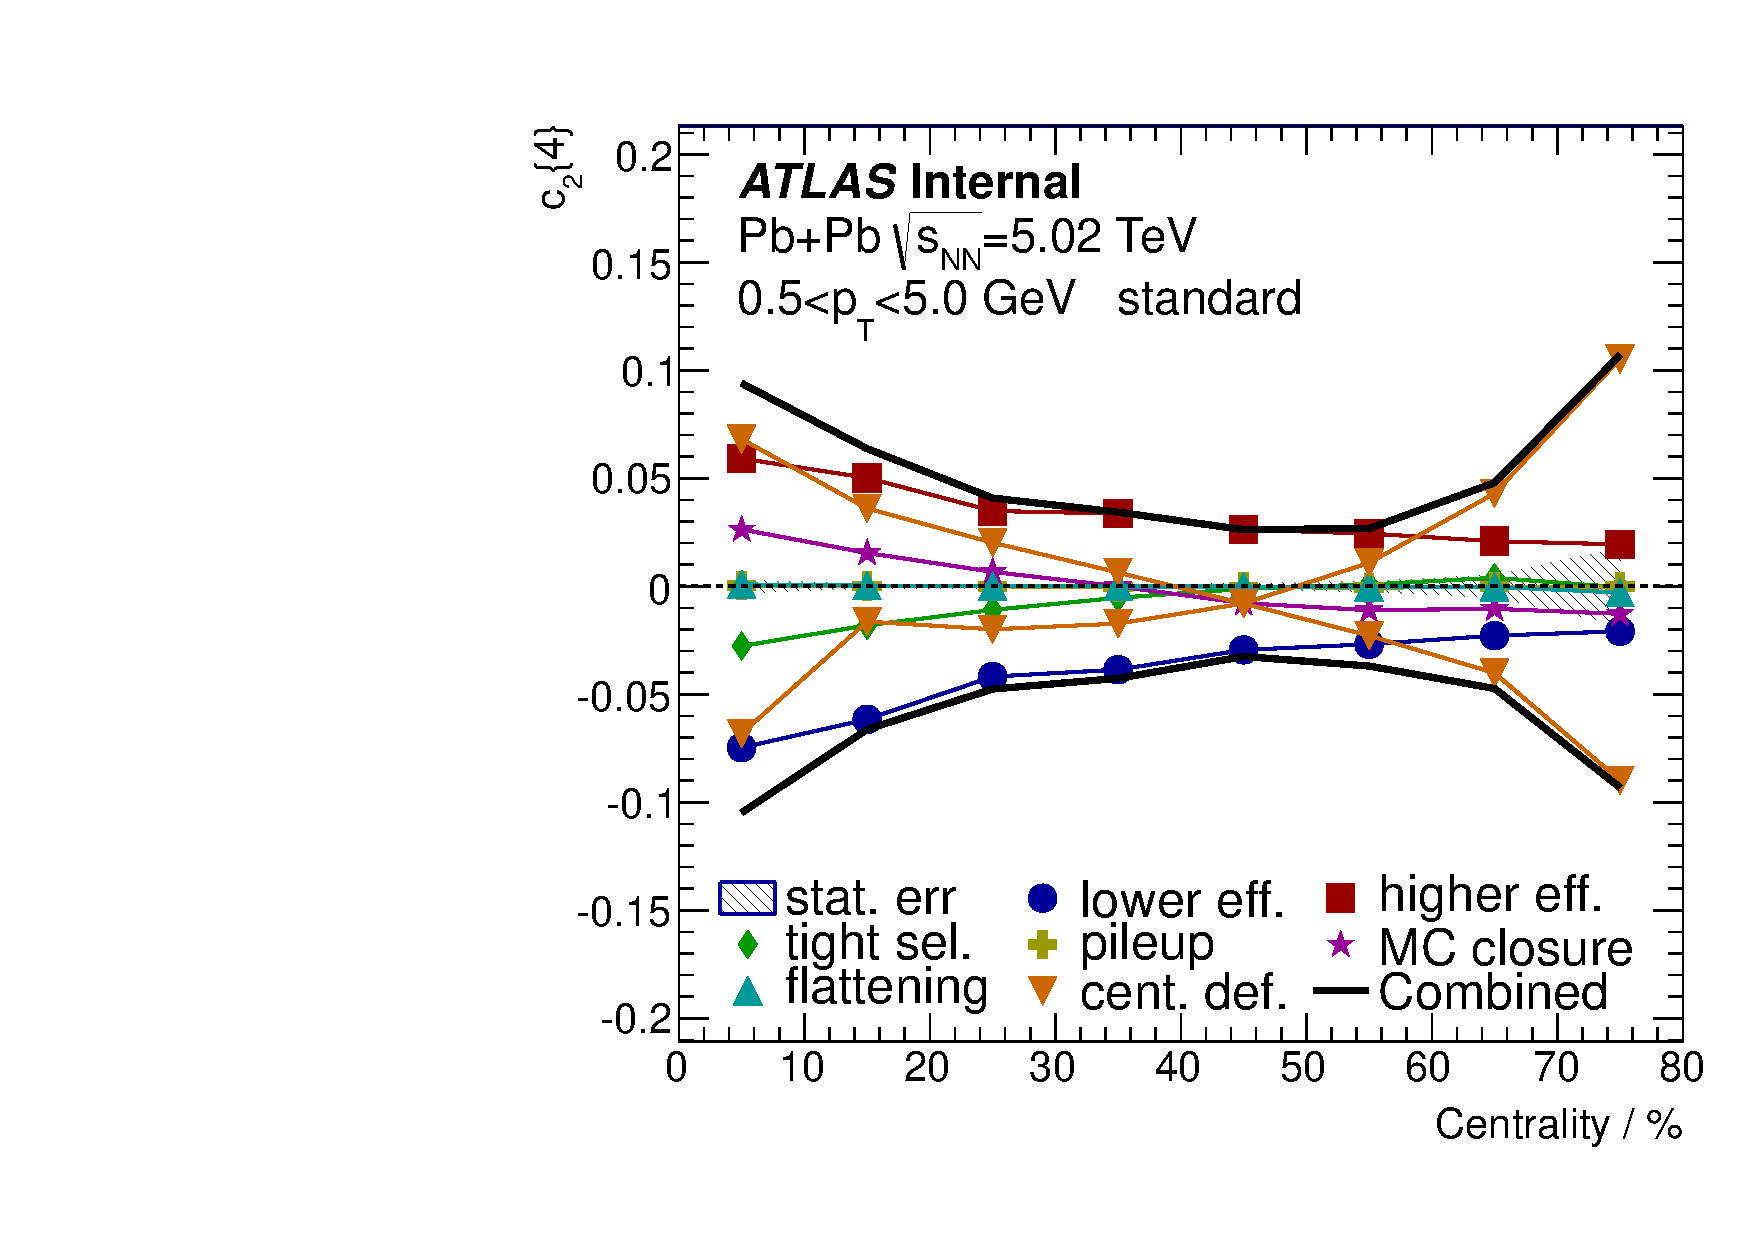
\includegraphics[width=.425\linewidth]{figs/chapter_appendix/sys_c4_1sub_Har2_Pt0.pdf}
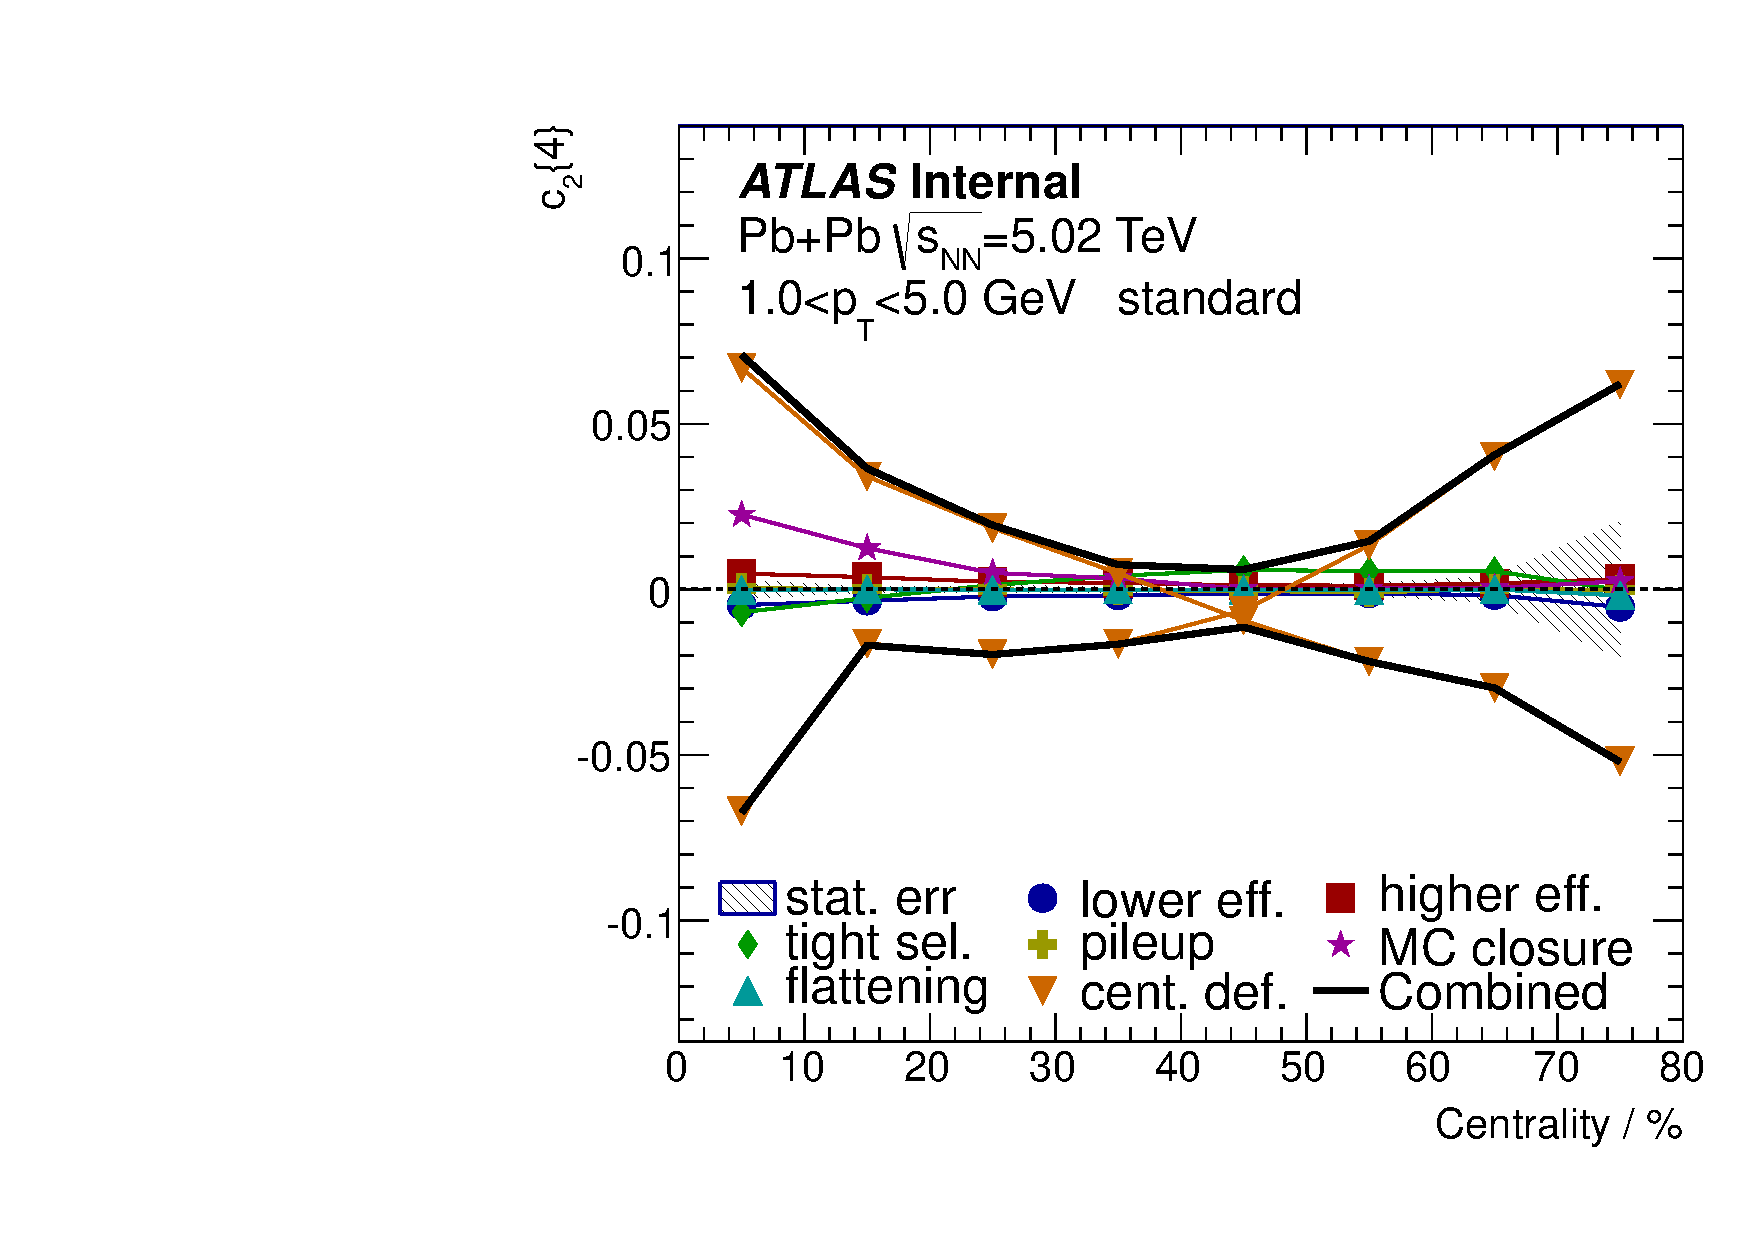
\includegraphics[width=.425\linewidth]{figs/chapter_appendix/sys_c4_1sub_Har2_Pt1.pdf}
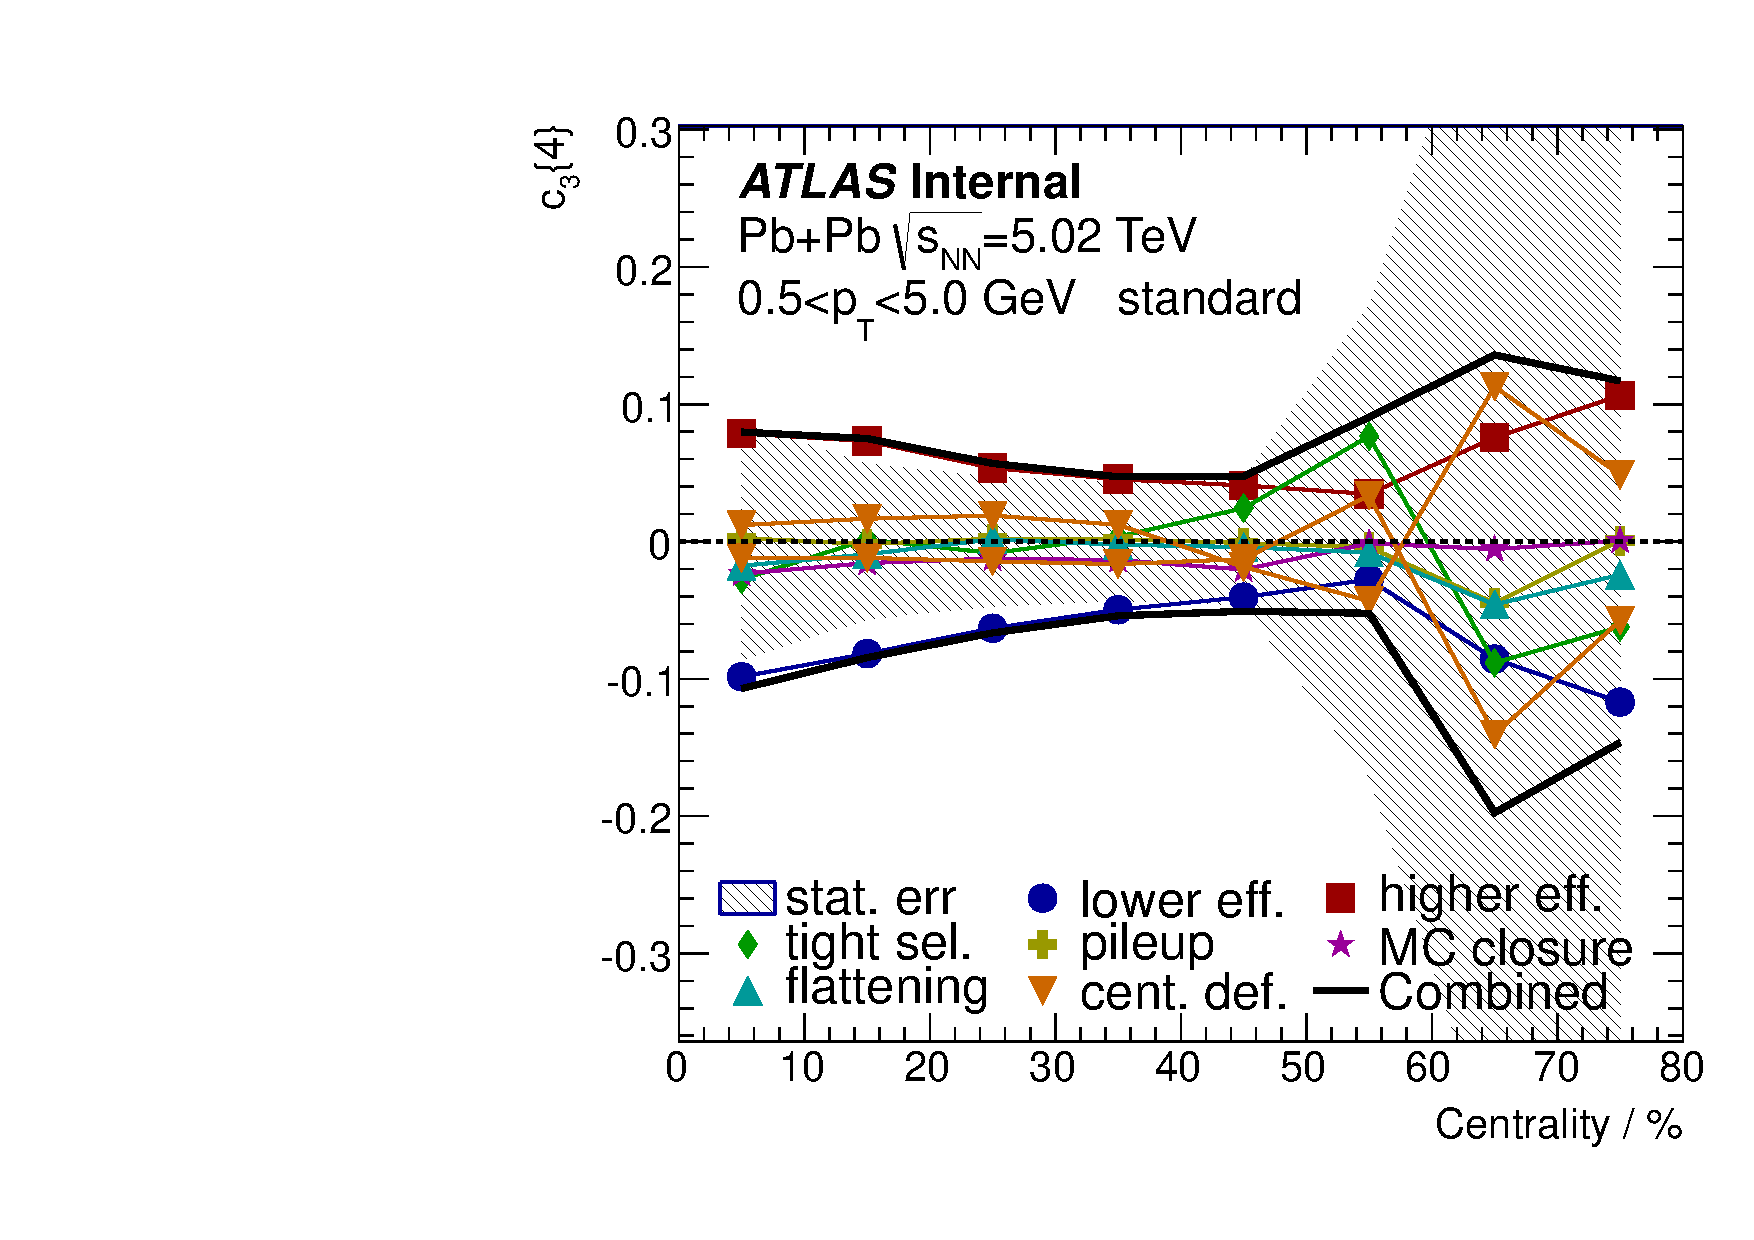
\includegraphics[width=.425\linewidth]{figs/chapter_appendix/sys_c4_1sub_Har3_Pt0.pdf}
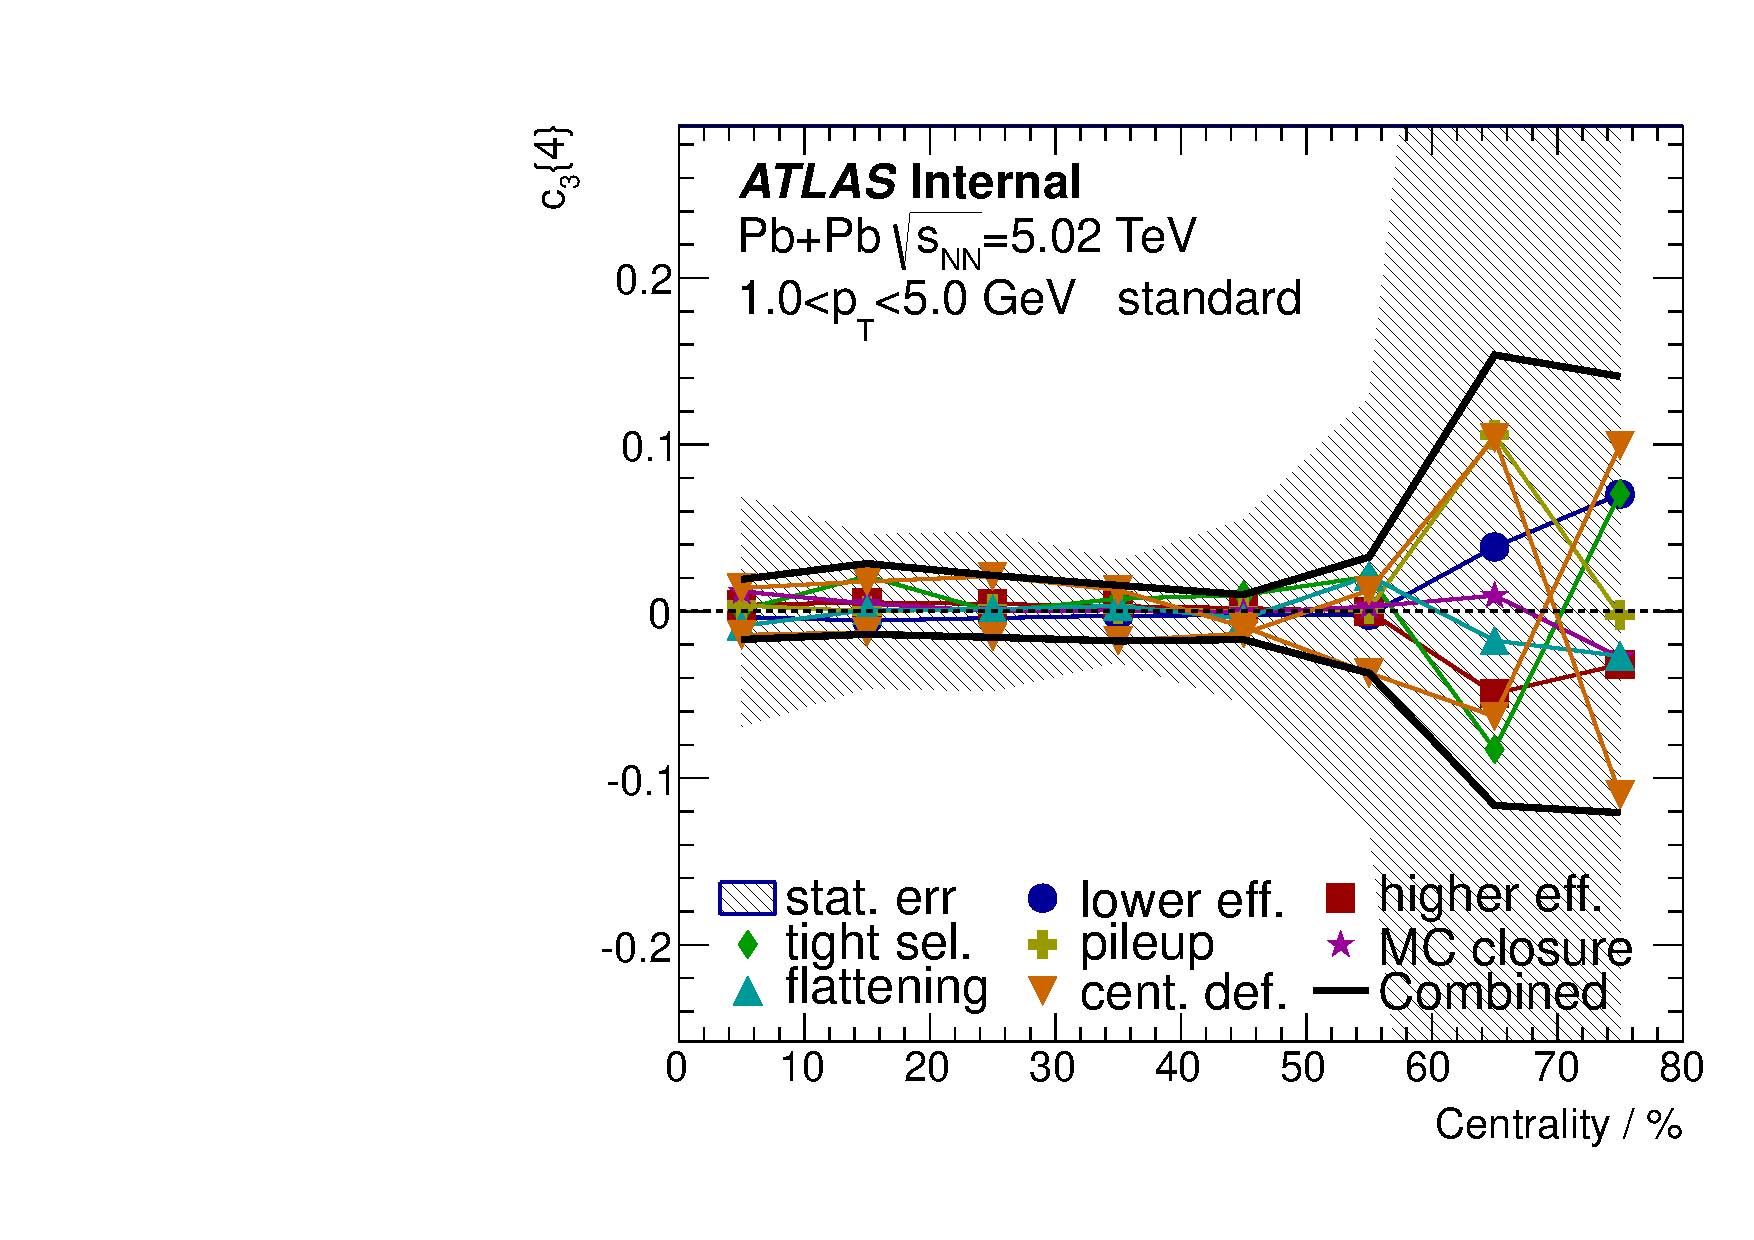
\includegraphics[width=.425\linewidth]{figs/chapter_appendix/sys_c4_1sub_Har3_Pt1.pdf}
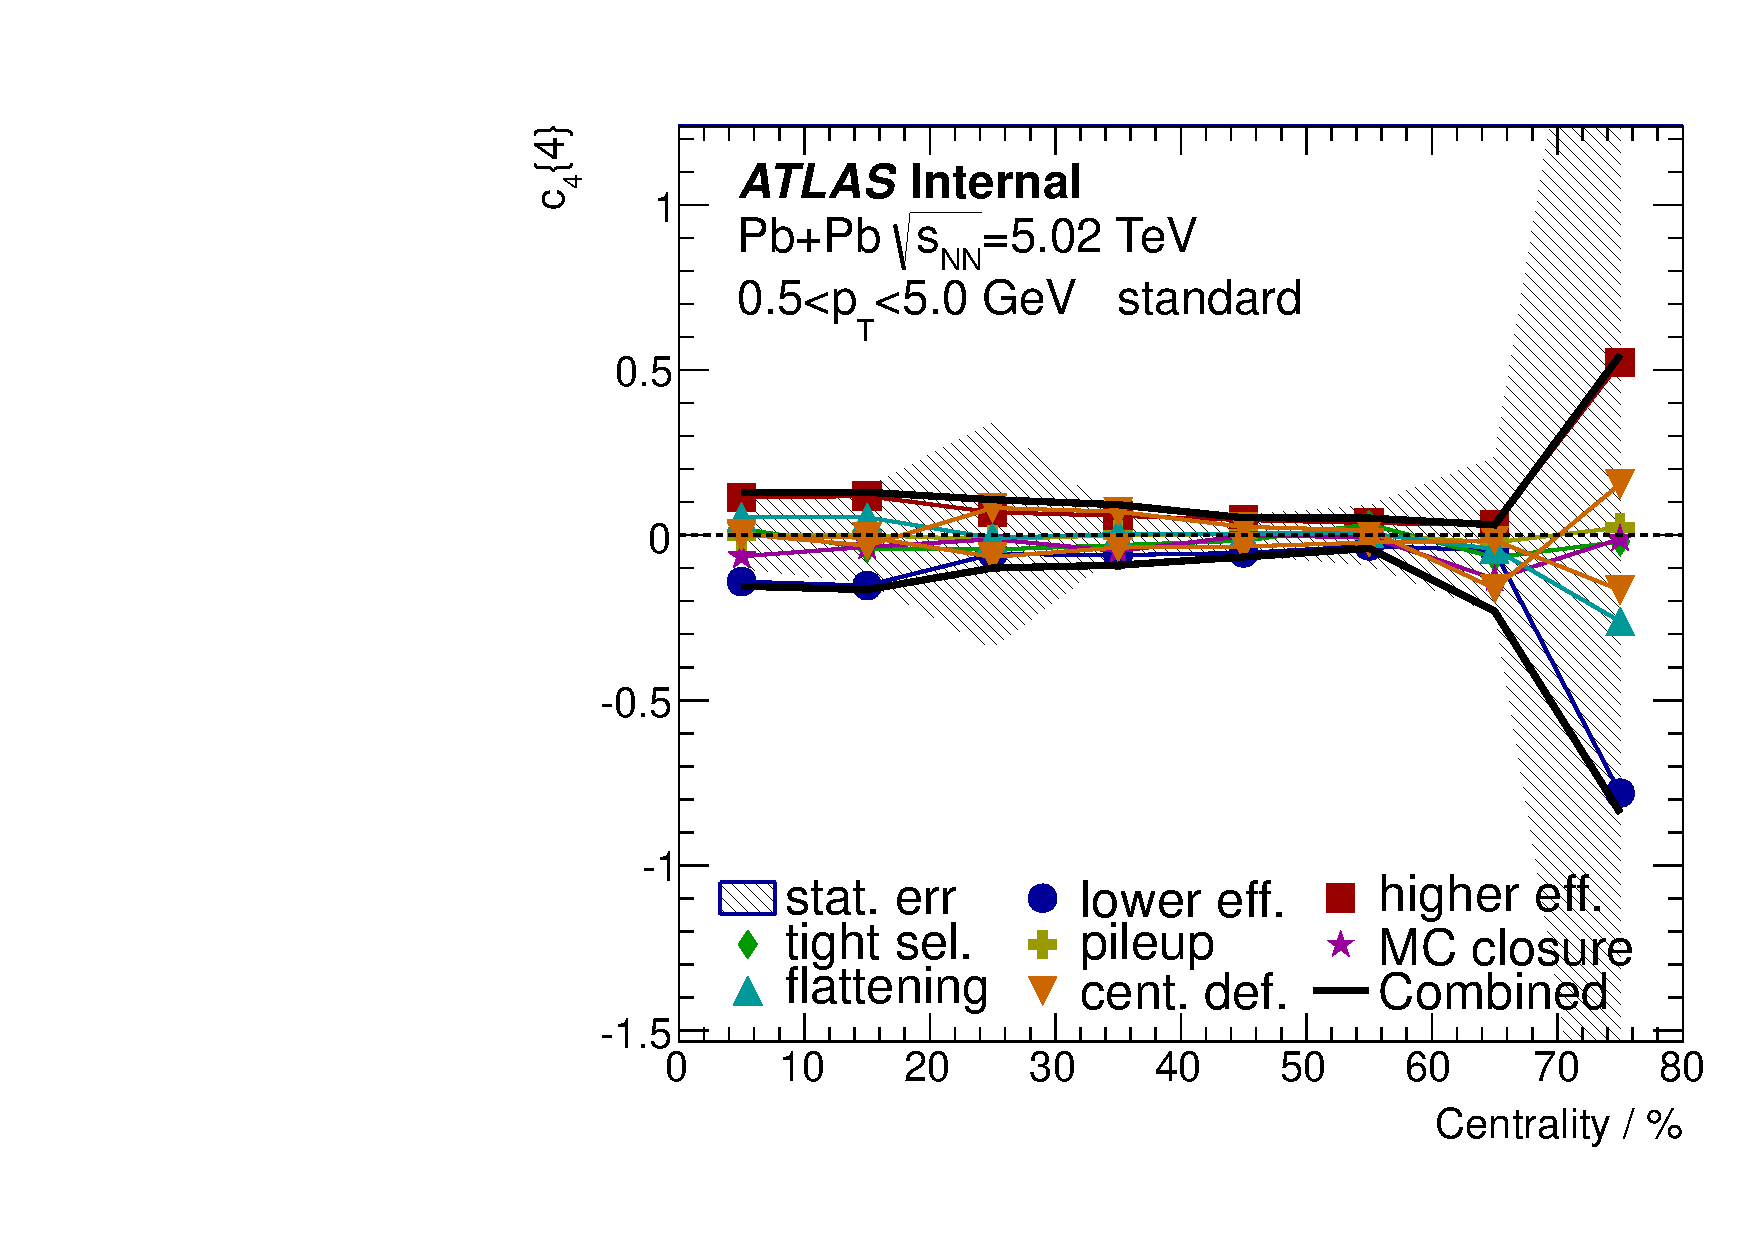
\includegraphics[width=.425\linewidth]{figs/chapter_appendix/sys_c4_1sub_Har4_Pt0.pdf}
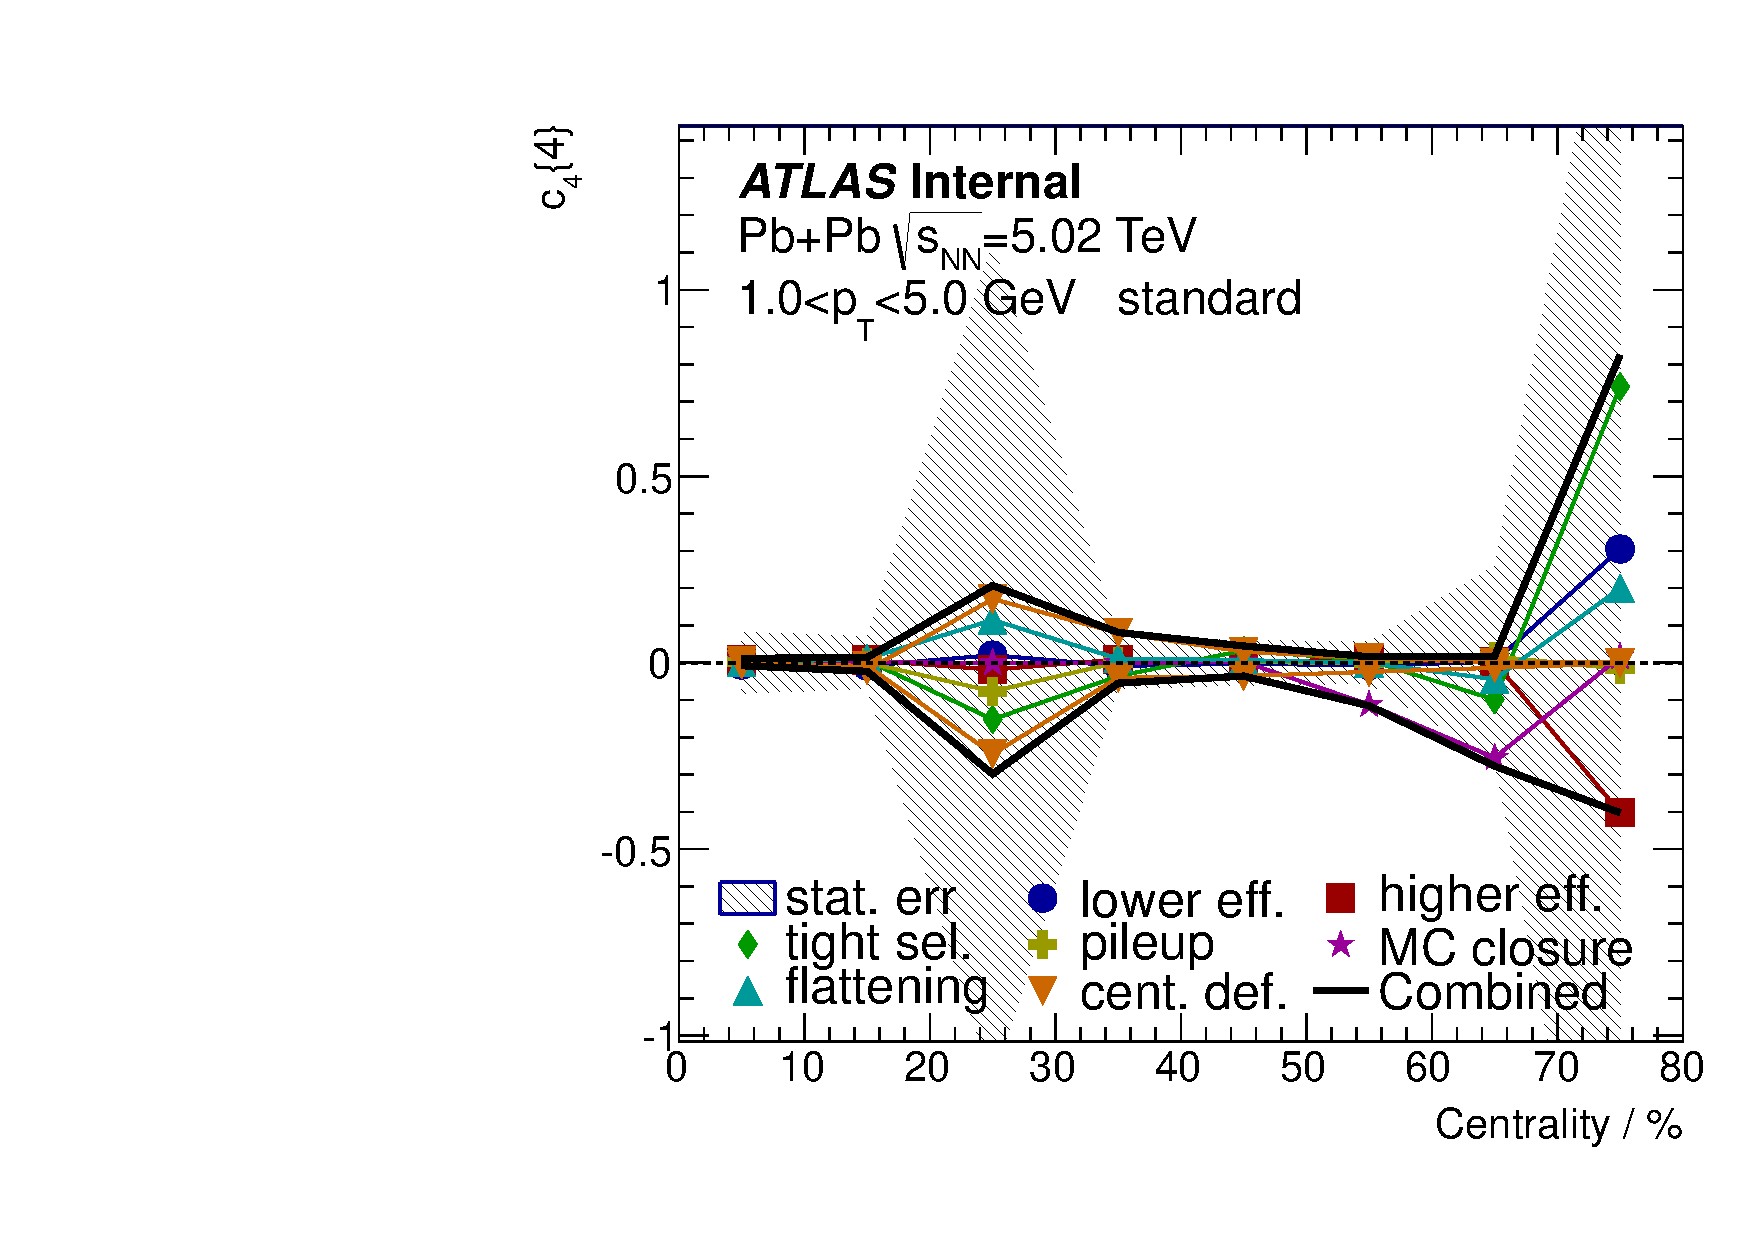
\includegraphics[width=.425\linewidth]{figs/chapter_appendix/sys_c4_1sub_Har4_Pt1.pdf}
\caption{Breakdown of all major systematic sources for 4-particle cumulant $c_n\{4\}$. Left column shows the lower $\pT$ cut and right column shows the higher $\pT$ cut. Different rows represent different harmonics. The cumulants are calculated using standard method. Shaded area indicate the statistical uncertainty.}
\end{figure}

\begin{figure}[H]
\centering
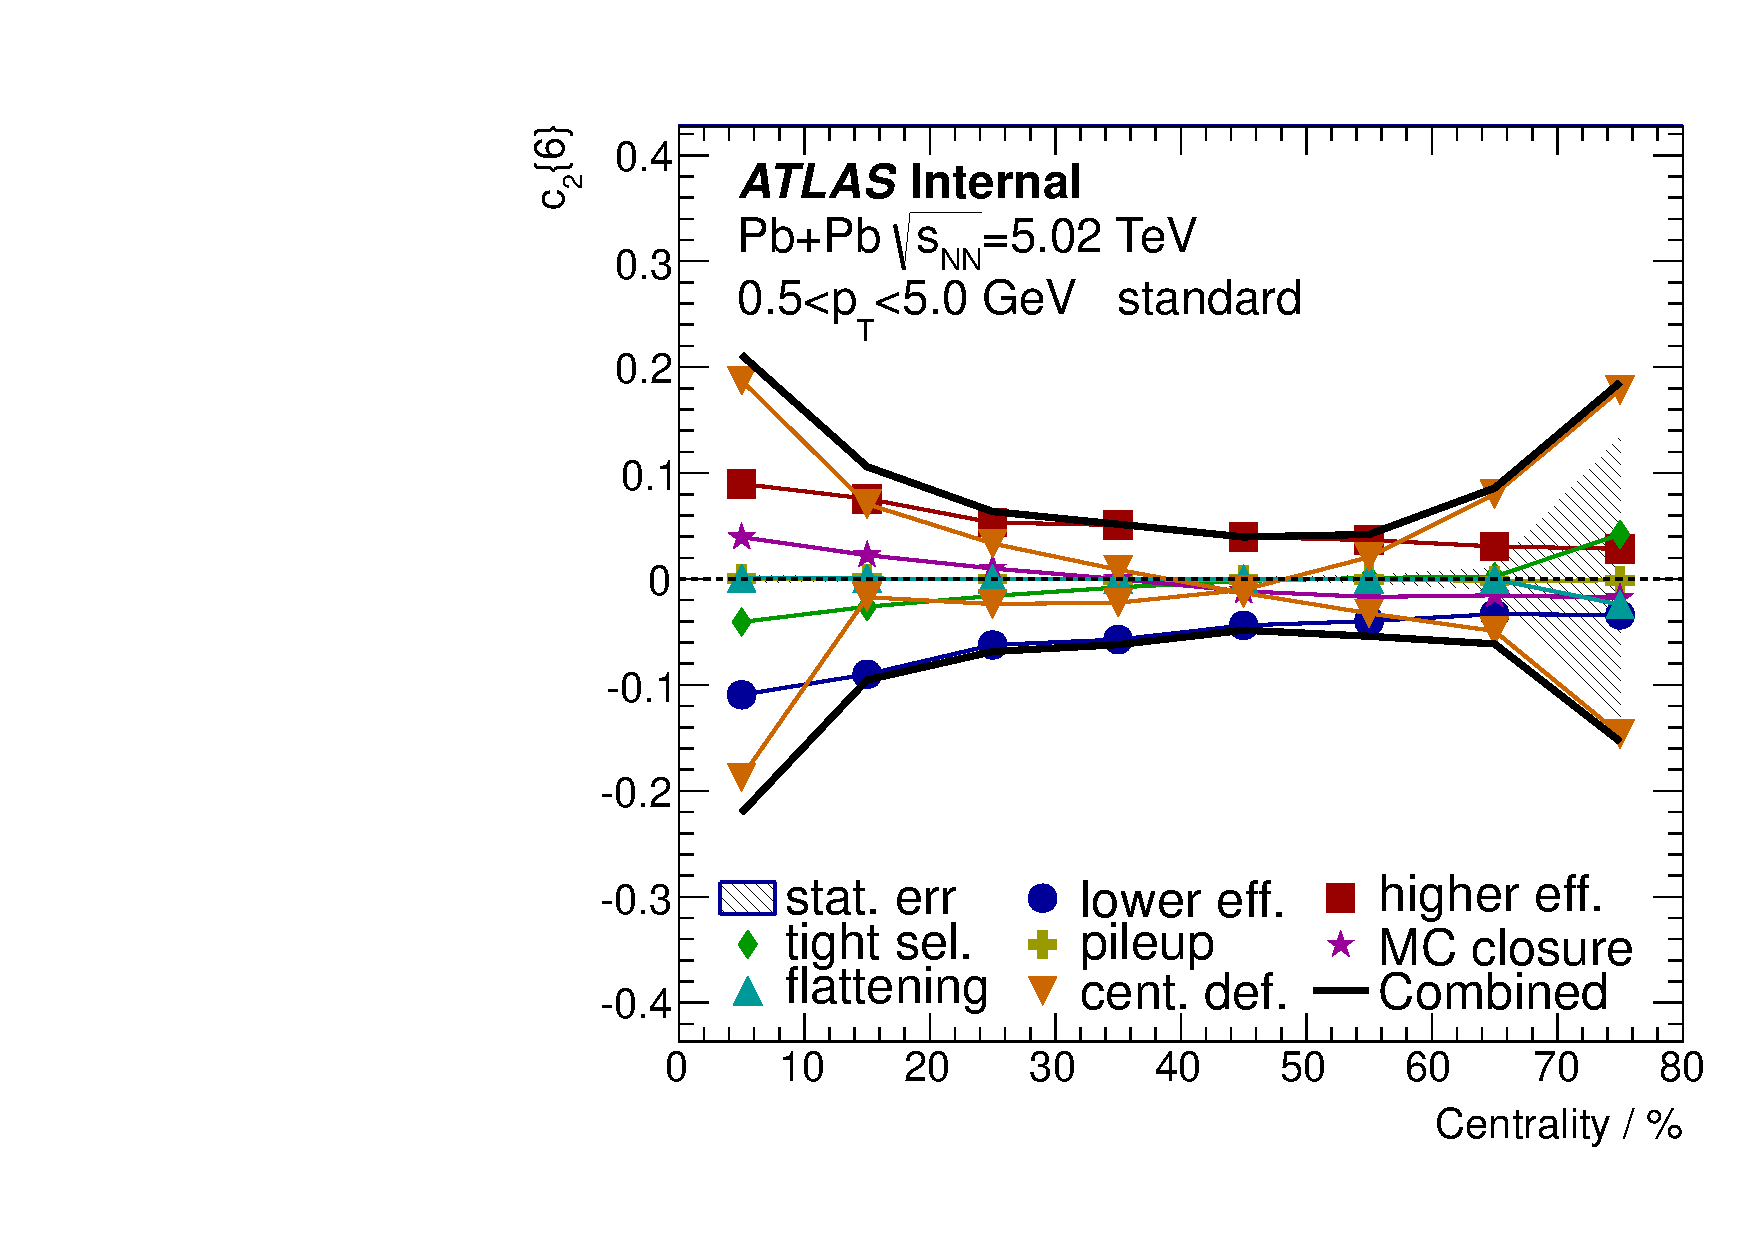
\includegraphics[width=.425\linewidth]{figs/chapter_appendix/sys_c6_1sub_Har2_Pt0.pdf}
\includegraphics[width=.425\linewidth]{figs/chapter_appendix/sys_c6_1sub_Har2_Pt1.pdf}
\includegraphics[width=.425\linewidth]{figs/chapter_appendix/sys_c6_1sub_Har3_Pt0.pdf}
\includegraphics[width=.425\linewidth]{figs/chapter_appendix/sys_c6_1sub_Har3_Pt1.pdf}
\includegraphics[width=.425\linewidth]{figs/chapter_appendix/sys_c6_1sub_Har4_Pt0.pdf}
\includegraphics[width=.425\linewidth]{figs/chapter_appendix/sys_c6_1sub_Har4_Pt1.pdf}
\caption{Breakdown of all major systematic sources for 6-particle cumulant $c_n\{6\}$. Left column shows the lower $\pT$ cut and right column shows the higher $\pT$ cut. Different rows represent different harmonics. The cumulants are calculated using standard method. Shaded area indicate the statistical uncertainty.}
\end{figure}

\begin{figure}[H]
\centering
\includegraphics[width=.425\linewidth]{figs/chapter_appendix/sys_sc_1sub_Har2_Pt0.pdf}
\includegraphics[width=.425\linewidth]{figs/chapter_appendix/sys_sc_1sub_Har2_Pt1.pdf}
\includegraphics[width=.425\linewidth]{figs/chapter_appendix/sys_sc_1sub_Har3_Pt0.pdf}
\includegraphics[width=.425\linewidth]{figs/chapter_appendix/sys_sc_1sub_Har3_Pt1.pdf}
\caption{Breakdown of all major systematic sources for symmetric cumulant $sc_{n,m}\{4\}$. Left column shows the lower $\pT$ cut and right column shows the higher $\pT$ cut. Different rows represent different harmonic combinations. The cumulants are calculated using standard method. Shaded area indicate the statistical uncertainty.}
\end{figure}

\begin{figure}[H]
\centering
\includegraphics[width=.425\linewidth]{figs/chapter_appendix/sys_ac_1sub_Har2_Pt0.pdf}
\includegraphics[width=.425\linewidth]{figs/chapter_appendix/sys_ac_1sub_Har2_Pt1.pdf}
\caption{Breakdown of all major systematic sources for asymmetric cumulant $ac_{n,n+m}\{3\}$. Left column shows the lower $\pT$ cut and right column shows the higher $\pT$ cut. The cumulants are calculated using standard method. Shaded area indicate the statistical uncertainty.}
\end{figure}



